\documentclass{article}

% --------------------
% Packages
% --------------------
\usepackage{graphicx}
\usepackage[a4paper, margin=1in]{geometry}
\usepackage{amsmath}

\usepackage[
    backend=biber,
    style=authoryear,
    maxcitenames=2,
    uniquelist=false,
    uniquename=false,
    maxbibnames=3
]{biblatex}
\addbibresource{references.bib}

\usepackage{booktabs}
\usepackage{array}
\usepackage{longtable}
\usepackage{float}

% Hyperlinks
\usepackage[hidelinks]{hyperref}

% --------------------
% Custom commands
% --------------------
\usepackage[hidelinks]{hyperref}

\newcommand{\githuburl}{https://github.com/KasLoot/RoboPref}
\newcommand{\resultsurl}{https://liveuclac-my.sharepoint.com/:u:/g/personal/ucabibp_ucl_ac_uk/IQCUJvx2H20nSIxwF1vrFhgmAYJn0NPS3Deujkp-VIlDPq8?e=BPVJlf}

\newcolumntype{P}[1]{>{\raggedright\arraybackslash}p{#1}}

% --------------------
% Float spacing
% --------------------
\setlength{\intextsep}{7pt plus 2pt minus 2pt}
\setlength{\textfloatsep}{8pt plus 2pt minus 2pt}
\setlength{\floatsep}{8pt plus 2pt minus 2pt}
\setlength{\abovecaptionskip}{5pt}
\setlength{\belowcaptionskip}{0pt}

% --------------------
% Title information
% --------------------
\title{
    PrefMem: A Preference-Aware, Evidence-Gated Agentic System for
    Interactive Robot Manipulation with Ambiguous Instructions
    \\[0.6em]
    \large
    \href{\githuburl}{\texttt{Click to access the GitHub repository}}
    \\[0.3em]
    \href{\resultsurl}{\texttt{Click to access the experiment results}}
}

\author{Candidate Number: VGWF5}

\date{June 2026}


% ============================================================
% DOCUMENT
% ============================================================

\begin{document}

% ============================================================
% TITLE PAGE
% ============================================================

\begin{titlepage}

    \centering

    \vspace*{\fill}

    % --------------------
    % Main title
    % --------------------
    {\LARGE\bfseries
    PrefMem: A Preference-Aware, Evidence-Gated Agentic System for
    Interactive Robot Manipulation with Ambiguous Instructions
    \par}

    \vspace{2cm}

    % --------------------
    % Author information
    % --------------------
    {\large
    % \textbf{Author}\\[0.4cm]

    Candidate Number: VGWF5\\[0.3cm]

    MSc. Robotics and Artificial Intelligence\\
    Department of Computer Science\\
    University College London\\[0.8cm]



    \par}

    \vfill

    % --------------------
    % Disclaimer
    % --------------------
    \begin{minipage}{0.85\textwidth}

        \small

        \textbf{Disclaimer:}
        The report will be distributed to the internal and external
        examiners, but thereafter may not be copied or distributed
        except with permission from the author.

    \end{minipage}

    \vspace{1.5cm}

    {\large June 2026\par}

    \vspace*{\fill}

\end{titlepage}


% ============================================================
% SECOND TITLE / ABSTRACT PAGE
% ============================================================

\maketitle

\begin{abstract}
Vision-language-Action (VLA) models map language and visual observations to robot actions. However, user intentions often lie beyond single language instructions. Moreover, current works show that VLAs tend to remember training trajectories instead of understanding and following specific semantic instructions \cite{ni2026semanticvla}. When given a long-horizon task in a new environment, they often follow the training data trajectories rather than generalise to act in the new environment. There are works that exist, such as SemanticVLA \cite{ni2026semanticvla}, that try to make the VLA follow instructions with semantic understanding, and MeM \cite{torne2026mem} that enables memory summarization prompt fallbacks to extend VLA abilities for long-horizon tasks. However, they are VLA models with new architecture designs and require training. And MeM \cite{torne2026mem} uses temporal long-term memory to leverage long-horizon tasks with ambiguous instructions, it does not solve the problem of understanding user intention. 

This project, \textbf{PrefMem}, however, takes a different path, instead of trying to design and train a new VLA model. PrefMem solves user intention understanding and long-horizon task execution by designing an agentic system; PrefMem does not need training and can be used out-of-the-box. PrefMem offers a preference-aware, evidence-gated orchestration layer above an interchangeable action executor. PrefMem features five model-facing agents which support human interaction, preference memory, planning, step monitoring, and final validation, while a deterministic runtime and receding-horizon controller own goal identity, confirmation, task publication, state transitions, temporal evidence requirements, and bounded recovery.

PrefMem is evaluated using development, non-confirmatory experiments in a restricted tabletop domain. With one applicable scoped preference, autonomous correct goal resolution increased from 0/36 observations under empty Memory to 36/36 under populated Memory, while both conditions achieved 36/36 final goal correctness after permitted clarification. Conflicting preferences caused clarification before commitment in 36/36 observations, and a held-out override replication selected the conflicting historical destination in 0/36 observations. A 30-interaction lifecycle experiment nevertheless retained the focal preference at the delayed final probe in only 2/8 stores, exposing a free-text identity limitation. Production Monitor improved the registered host route from 12/36 to 22/36 paired observations, while production Validator prevented false completion in all 21 visibly incomplete states compared with 0/21 for a stop-after-actions control. In 12 MuJoCo simulation episodes, correct contracts and simulator-truth physical goals occurred in 12/12, all-strict grounding in 11/12, Validator completion in 9/12, and exact one-action strict chain in 8/12.

These results support the PrefMem design as an inspectable systems architecture with measurable boundary-specific effects and identifiable failure mechanisms.

\end{abstract}
\section{Introduction}
\subsection{Motivation}
General-purpose robot policies produce robotic actions from natural language instructions and visual observations. RT-1 Brohan et al. (2022) demonstrated that a Vision-Language-Model trained on a large, diverse real-robot dataset can acquire multi-task behaviour in scale. And, RT-2 Brohan et al. (2023) shows that semantic knowledge can transfer into control by represented robot actions as tokens and fine-tuning a VLM on robot action data. Then, OpenVLAKim et al. (2024) introduces a 7-billion parameter sized VLA, trained on 970,000 real-world robot demonstrations and increased 16.5 percent success rate on the RT-2-X across 29 tasks. Then Octo and Pi 0 models shows a different action decoder design using diffusion policy. These models motivate the conceptual executor abstraction considered by this project: an instruction and an image are encoded into a multimodal representation, from which an action head predicts a continuous action or action chunk in a closed loop.

The direct vision and language to action generation formulation is powerful, but it cannot do high-level task reasoning and making decisions. For example, a command “Tidy this up” is syntactically clear but still underdetermined for different person who gives the command, and it is too ambiguous without referring to a specific use case history or clarifying with the user. “Tidy this up” does not say where each object belongs. “Put the cube on my board” does not identify the board unless the robot can retrieve a scoped preference. And, “do the usual thing” is nonsense when there is no context in the current run. TidyBot \cite{wu2023tidybot} showes that a language-model-based system can infer household placement preferences from a few demostrations, and achieves 91.2\% accuracy on unseen benchmark objects and 85.0\% placement success on its real robot.
And, APRICOT \cite{wang2024apricot} shows that preference inference must be considered with physical constraints and decomposes the instruction into plausible explanations. PrefMem agrees that personalisation matters, and focuses on how preference evidence should be scoped, confirmed, preserved, and carried out into execution.

In long-horizon task execution, a multi-step plan generated from an the old observation will become stale after or even during each step’s execution. A real-world deployable system must adapt to dynamically changing environments. Research on grounded language planning has shown the importance of connecting semantic plans to affordances and feedback. SayCan \cite{ahn2022saycan} scores language-model proposals with skill value functions.
And ReAct \cite{yao2023react} interleaves reasoning with environment-facing actions and observations.
More recent hierarchical systems like HiRobot \cite{shi2025hirobot} and AgenticRobot \cite{yang2025agenticrobot} place a reasoning model above a low-level VLA or policy.


PrefMem adopts and enhances the architectural design of semantic reasoning, physical execution, and verification with a multi-agent system, then adds explicit preference-memory and confirmation boundaries. This design allows PrefMem to maintain a trustworthy task contract between a person and the underlying execution system. In real running, the system must decide which historical preference is applicable, know when not to decide, preserve a current explicit correction over old memory, prevent a speculative preview from becoming an action, reject stale planning results, rely on stable evidence after each actions, and reserve final completion for a separate validation route. These responsibilities are difficult to audit when they are implicit in a single model prompt. PrefMem makes them explicit through typed messages and distributes them to different sub-agents within the system.

\subsection{Research Problem and Aim}
\label{subsec:research-problem}
Existing work has separately studied preference inference, language-grounded
planning, hierarchical execution, policy memory, and visual verification.
This thesis studies the governance boundary connecting these concerns: how
retrieved preference evidence becomes an explicitly authorised physical goal,
and how that goal remains fixed while plans, actions, observations, and
recovery decisions evolve.

Let a user issue instruction \(u\) in observed scene \(o_t\), with user
identity \(i\), task scope \(s\), and memory store \(\mathcal{M}\). A useful
system must form a confirmed goal contract \(g\) and then select actions
\(a_t\) as observations evolve. The problem contains three interacting
sources of uncertainty:
\begin{enumerate}
    \item Semantic uncertainty: the instruction may omit an object, target, constraint, or preference.
    \item Historical uncertainty: retrieved records may be irrelevant, stale, mutually inconsistent, or incorrectly scoped.
    \item Execution uncertainty: grounding, control, observation, monitoring, and validation may disagree even when the intended goal is correct.
\end{enumerate}

Accordingly, the aim of this thesis is to design and evaluate an inspectable
orchestration layer that converts ambiguous, preference-conditioned user
requests into confirmed physical-goal contracts and governs their execution
through fresh planning, temporally fenced evidence, bounded recovery, and
independent final validation. The thesis addresses the following research
questions:
\begin{enumerate}
    \item To what extent does one applicable user- and task-scoped preference reduce clarification requirements while preserving final goal correctness?
    \item Under what memory conditions does PrefMem abstain from autonomous commitment, and how reliably does it preserve explicit current instructions over historical defaults?
    \item How reliably does the implemented preference lifecycle preserve user, task, record, and value identity through creation, retrieval, update, intervening mutations, and revocation?
    \item What boundary-specific effects do production Monitor and Validator have relative to their registered controls?
    \item To what extent can a confirmed preference-conditioned contract reach its registered MuJoCo final state, and which component boundaries explain unsuccessful strict completion?
\end{enumerate}

\subsection{Contribution}
This thesis has the following contributions.
\begin{enumerate}
    \item A five-agent orchestration architecture separating human interaction, preference memory, planning, step monitoring, and final validation from an interchangeable physical executor.

    \item A deterministic trust boundary in which models propose semantic content while host code owns goal identity and revision, exact confirmation, lifecycle state, an execution horizon of one, publication fencing, temporal evidence aggregation, loop guards, and terminal state.

    \item A conservative preference-memory policy combining retrieval before mutation, bounded candidate injection, semantic applicability filtering, explicit future-facing consent, and at most one justified mutation per interaction.

    \item A confirmed execution contract consisting of an immutable goal and frozen validation checklist, with step-level monitoring, fresh replanning after terminal results, and a separate whole-goal completion gate.

    \item A layered evaluation methodology that reports direct component, interface, ablation, robustness, and end-to-end outcomes while preserving null and negative evidence and avoiding a misleading global system score.
\end{enumerate}




\section{Related Work}
\label{sec:related-work}

PrefMem lies at the intersection of language-conditioned robot control,
personalised assistance, interactive task specification, long-horizon
orchestration, and visual verification. These areas address different
responsibilities. A robot policy determines how an instruction should be
realised through actions, whereas an orchestration system must additionally
determine whether the instruction is sufficiently specified, which historical
information is authorised and applicable, what exact outcome the user has
confirmed, and what evidence permits the system to advance or terminate. This
section therefore distinguishes action-generation capability from task-level
governance and positions PrefMem as a complementary layer above an
interchangeable executor.

\subsection{Language-Conditioned Robot Policies and VLAs}
\label{subsec:related-vla}

Large-scale language-conditioned robot policies established that diverse
robot data and high-capacity architectures can support multi-task behaviour.
RT-1 introduced a transformer-based policy trained on a large collection of
real-robot trajectories and studied how performance varied with model
capacity, dataset size, and task diversity
\parencite{brohan2022rt1}. RT-2 subsequently formulated robot actions as text
tokens and co-fine-tuned vision--language models on robot trajectories and
Internet-scale vision--language tasks
\parencite{brohan2023rt2}. This allowed semantic knowledge acquired during
vision--language pretraining to influence action generation, including
generalisation to previously unseen object categories, linguistic references,
and elementary reasoning tasks.

Related work has explored embodied reasoning without directly treating the
model as a complete action policy. PaLM-E injects continuous sensor
representations into a large language model and jointly trains across embodied
reasoning, visual question answering, and language tasks
\parencite{driess2023palme}. It demonstrates that multimodal foundation models
can integrate physical observations with semantic reasoning, but does not
imply that the same model must own task authorisation, persistent user
preferences, or the complete robot lifecycle.

OpenVLA provides an open 7-billion-parameter VLA based on a Llama 2 language
backbone and fused DINOv2 and SigLIP visual features
\parencite{kim2024openvla}. It was trained on approximately 970,000 real-world
robot demonstrations and demonstrated efficient adaptation to new tasks.
Continuous-action architectures have developed alongside token-based methods.
The \(\pi_0\) model combines a pretrained vision--language backbone with a
flow-matching action expert and trains across single-arm, dual-arm, and mobile
manipulator embodiments \parencite{black2025pi0}. This formulation supports
continuous action chunks for dexterous behaviours while retaining semantic
conditioning from the vision--language backbone.

More recent systems increase the scale and steerability of the policy itself.
LingBot-VLA reports pretraining on approximately 20,000 hours of real-world
data from nine dual-arm configurations and evaluates transfer across multiple
robot platforms \parencite{wu2026pragmaticvla}. The later
\(\pi_{0.7}\) model conditions action generation on a richer multimodal
context, including subtask instructions, generated subgoal images, control
mode, and episode-quality metadata
\parencite{physicalintelligence2026pi07}. This detailed conditioning allows
data containing different strategies, qualities, and embodiments to be used
without requiring the policy to average them into a single undifferentiated
behaviour.

These advances make it inappropriate to motivate PrefMem through a categorical
claim that VLAs cannot reason or generalise. Modern VLAs increasingly support
language understanding, continuous control, memory, and multi-stage
behaviour. The remaining problem addressed in this thesis is different: a
capable action policy does not by itself define how persistent preference
evidence becomes an authorised goal, how a user confirms that goal, or how
task-level evidence is fenced and audited across execution.

\subsection{Semantic Reasoning Within VLAs}
\label{subsec:related-semantic-vla}

A growing body of work studies how the semantic capabilities of a pretrained
vision--language model can be preserved or strengthened during action
training. One challenge is that optimisation on robot trajectories may cause
catastrophic forgetting or encourage the backbone to correlate familiar
visual and linguistic patterns directly with actions. This can reduce the
benefit of the pretrained model's broader reasoning capabilities.

InstructVLA addresses this problem through Vision--Language--Action
Instruction Tuning, a two-stage training procedure that combines multimodal
reasoning data, embodied instruction annotations, mixture-of-experts
adaptation, and flow-based action generation
\parencite{yang2025instructvla}. Its instruction-tuning data include scene
descriptions, question answering, command rewriting, and implicit task
contexts. Consequently, the model is trained not only to execute atomic
instructions but also to interpret paraphrases, attributes, negation, and
higher-level task descriptions.

SemanticVLA similarly studies the tension between semantic reasoning and
action-pattern memorisation
\parencite{ni2026semanticvla}. It introduces two complementary intermediate
representations. Explicit trace reasoning generates interpretable spatial
waypoints through the language interface, while latent action tokens encode
compact, visually grounded manipulation primitives. Both signals condition a
flow-matching action decoder. Its instruction-rephrasing experiments are
particularly relevant because they evaluate whether semantically equivalent
instructions continue to produce appropriate actions rather than merely
matching wording observed during training.

These methods improve reasoning \emph{inside} the execution policy. PrefMem
instead externalises several task-level decisions. Its preference provenance,
goal confirmation, publication identities, execution history, and final
completion report remain inspectable even when the executor uses opaque latent
representations. The approaches are therefore complementary: an executor such
as InstructVLA, SemanticVLA, or \(\pi_{0.7}\) could replace PrefMem's current
execution surrogate without changing the upper-level goal, evidence, or
control contracts.

\subsection{Personalised Robot Assistance and Preference Learning}
\label{subsec:related-personalisation}

Personalised assistance requires a robot to distinguish a user's habitual
choices from generic commonsense. TidyBot studies this problem in household
cleanup, where the correct receptacle and manipulation primitive depend on
individual preferences \parencite{wu2023tidybot}. The system uses an LLM to
summarise a small set of example placements into general rules and applies
those rules to unseen objects. This demonstrates that language models can
generalise personalised placement patterns from limited examples. However,
its principal research question is preference generalisation, rather than the
lifecycle and authority of individual persistent records.

LLM-Personalize adapts an LLM planner to household preferences through
imitation learning and reinforced self-training
\parencite{han2024llmpersonalize}. The planner acts iteratively in partially
observable Housekeep environments using a dynamically constructed scene graph.
An initial imitation-learning phase teaches executable planning and preliminary
preference alignment, after which self-training explores and reinforces
preference-compatible plans. In this case, personalisation is incorporated
through model optimisation. This differs from PrefMem, which keeps the
underlying conversational and action models fixed and represents preferences
as explicit, inspectable records.

APRICOT combines LLM-based Bayesian active preference learning with
constraint-aware task planning \parencite{wang2024apricot}. Visual
demonstrations are converted into language descriptions and used to construct
candidate preference hypotheses. When uncertainty remains, the system selects
questions intended to reduce the posterior uncertainty over those candidates.
A task planner then refines its proposed arrangement using geometric feedback
from a world model. APRICOT therefore connects preference inference, active
questioning, and physical feasibility. Its active-learning formulation assumes
that an adequate explanation is represented among the candidate preferences,
whereas PrefMem treats missing or conflicting applicable records as reasons to
abstain and request direct clarification.

PrefMem does not attempt to infer a general reward function or retrain a
personalised planner from demonstrations. It instead addresses persistent
preference governance: records are retrieved under user and task scope,
filtered for semantic applicability, mutated only through an explicit memory
operation, and never created merely because the user confirmed the current
task. A current instruction has field-level priority over historical defaults.
Thus, the central distinction is between \emph{learning what a user probably
prefers} and \emph{deciding whether an existing preference record is
authorised, applicable, and sufficient for the present physical task}.

\subsection{Ambiguity, Clarification, and Human Assistance}
\label{subsec:related-ambiguity}

A robot should not resolve every uncertain instruction by guessing, but asking
for help on every task would make the system unnecessarily dependent on the
user. KnowNo formalises this trade-off as uncertainty alignment for
language-model planners \parencite{ren2023knowno}. It uses conformal
prediction to construct a calibrated set of candidate actions. A singleton set
allows autonomous execution, whereas a larger set causes the robot to ask the
user for help. Under its calibration assumptions, this provides a
user-specified coverage level while reducing unnecessary intervention.

KnowNo is an important comparison because it provides a formal uncertainty
guarantee, which PrefMem does not. Its guarantee assumes, among other
conditions, that the relevant environment entities are grounded in the
planner's input and that the proposed low-level actions can be executed
successfully. PrefMem instead separates semantic, historical, and execution
uncertainty. It may clarify because a task field is missing, because retrieved
records conflict, because the Planner reports a capability boundary, or
because monitoring and validation cannot obtain sufficient evidence.
Clarification and attention are governed by typed system states and semantic
policy rather than a calibrated conformal prediction set.

APRICOT and KnowNo both show that question asking should be selective rather
than universal. PrefMem follows the same interaction principle at a narrower
preference-memory boundary. One uniquely applicable record may provide a
default for a missing field; an empty, irrelevant, or conflicting result
requires a focused question. Regardless of whether clarification was required,
PrefMem subsequently asks the user to confirm the exact staged goal identifier
and revision. This confirmation is an authorisation boundary and should not be
confused with statistical uncertainty calibration.

\subsection{Language Planning and Agentic Robot Orchestration}
\label{subsec:related-orchestration}

Language-model planning systems often combine semantic proposals with
embodiment-specific constraints. SayCan scores language-model skill proposals
using value functions associated with executable robot skills
\parencite{ahn2022saycan}. The language model contributes semantic knowledge
about how a task may be decomposed, while the value functions ground this
knowledge in the robot's available capabilities and current environment.
Code as Policies instead prompts a language model to generate programs that
compose perception and control APIs
\parencite{liang2022codeaspolicies}. These programs can express geometric
reasoning, feedback loops, and reusable hierarchical functions.

Closed-loop feedback is necessary because an initially plausible plan may
become invalid during execution. Inner Monologue feeds scene descriptions,
success-detector outputs, and human feedback back into a language planner
\parencite{huang2022innermonologue}. This enables the planner to revise its
decisions as execution changes the environment. ReAct provides a broader
language-agent formulation in which reasoning traces are interleaved with
environment-facing actions and observations
\parencite{yao2023react}. Although ReAct is not specifically a robot-control
architecture, its reasoning--acting loop influenced later agentic systems.

Hi Robot explicitly divides robot control into a high-level VLM and a
low-level VLA \parencite{shi2025hirobot}. The high-level model interprets
complex user prompts, visual observations, and mid-task feedback, then produces
simpler instructions for the low-level policy. Its evaluation demonstrates the
value of hierarchy for situated corrections and compositional instructions.
The high-level policy is invoked at a lower frequency or in response to user
feedback, while the low-level policy continuously produces action chunks.

Agentic Robot introduces a Planner--Executor--Verifier architecture governed by
a Standardized Action Procedure
\parencite{yang2025agenticrobot}. A reasoning model decomposes a task into
atomic subgoals, a VLA executes each subgoal, and a temporal VLM verifier
determines whether execution should continue, retry, or recover. This work is a
close architectural precedent for PrefMem because it treats verification as a
control signal rather than an offline metric.

RoboClaw extends agentic orchestration across the robot learning lifecycle
\parencite{li2026roboclaw}. A VLM meta-controller reasons over observations,
task memory, working memory, and a tool interface to select and monitor learned
skill policies. Forward and inverse policies form self-resetting data-collection
loops, while deployment trajectories can later refine the policy library.
RoboClaw therefore connects orchestration with continued data acquisition and
policy improvement.

PrefMem adopts the general lesson that semantic planning, execution, and
verification benefit from explicit interfaces, but introduces different
authority and temporal semantics. The Planner may predict several candidate
tasks, yet deterministic host code publishes only the first, producing an
execution horizon of one. After each stable terminal step result, a new frame
and immutable execution history are used to request a fresh plan toward the
same frozen goal. In contrast to RoboClaw, PrefMem does not update policy
weights from deployment experience. In contrast to systems that rely only on
an initially decomposed subgoal sequence, PrefMem discards the unexecuted
prediction tail and replans after every terminal task observation.

\subsection{Memory Across Robot Interaction}
\label{subsec:related-memory}

The term \emph{memory} describes several distinct mechanisms in embodied
systems. A policy may require short-term visual memory to handle occlusion,
within-episode semantic memory to track completed subtasks, or persistent
declarative memory describing a user's preferences across separate
interactions. Treating these mechanisms as interchangeable obscures both their
authority and their failure modes.

Multi-Scale Embodied Memory (MEM) combines a video-based short-horizon memory
with a compressed language-based long-horizon memory inside a VLA
\parencite{torne2026mem}. The video encoder retains fine-grained recent
information needed for dynamics, re-grasping, and self-occlusion. A high-level
policy maintains a textual summary of relevant events, such as which recipe
steps have been completed or which doors remain open. This permits the policy
to act over tasks lasting many minutes without passing the complete dense
observation history into every inference call.

RoboClaw similarly distinguishes task-level and working memory. Its task
memory records global progress, whereas working memory records the currently
active skill and tool history \parencite{li2026roboclaw}. These forms of memory
support execution context. TidyBot and APRICOT, by comparison, represent
information about a user's desired organisation rules
\parencite{wu2023tidybot,wang2024apricot}.

PrefMem contains both task history and preference memory, but keeps them under
different contracts. Terminal execution records are host-owned, immutable
evidence supplied to future planning cycles. Persistent preference records are
stored separately and may be retrieved, remembered, updated, or forgotten only
through the Memory boundary. Conversation history is evidence for a question;
it is not automatically converted into a persistent default. This separation
is central to the thesis because a record of what happened during one task
does not, by itself, authorise the robot to treat that event as the user's
future preference.

\subsection{Monitoring, Verification, and Goal Completion}
\label{subsec:related-verification}

Execution feedback can serve several purposes. A success detector may indicate
that the next subgoal can begin, a verifier may identify a failed grasp and
trigger recovery, and a task-level evaluator may determine whether the user's
complete request has been satisfied. Prior closed-loop systems primarily
emphasise the first two responsibilities. Inner Monologue incorporates success
detections into replanning \parencite{huang2022innermonologue}; Agentic Robot
uses a temporal verifier to decide whether to continue, retry, or recover
\parencite{yang2025agenticrobot}; and RoboClaw periodically queries robot and
environment state to supervise skill execution
\parencite{li2026roboclaw}.

These mechanisms address the limitations of open-loop progression, but local
subgoal success is not logically equivalent to whole-goal completion. A robot
may successfully place one object while violating a required order, disturbing
another completed arrangement, or leaving part of the original request
unfinished. Conversely, an occluded or ambiguous view should not automatically
be interpreted as physical failure.

PrefMem therefore separates two visual authorities. Monitor evaluates only the
single active step and its expected observations using post-publication
evidence. Validator evaluates an immutable checklist derived from the complete
confirmed goal. The checklist is frozen before execution, preventing later
failures from weakening the success criteria. Validator may accumulate
criterion evidence over multiple views, while deterministic host code derives
whether the outcome is complete, incomplete, or still requires evidence. This
separation is intended to prevent attempted actions or a count of successful
subtasks from being treated as proof of overall completion.

\subsection{Positioning of PrefMem}
\label{subsec:related-positioning}

Table~\ref{tab:related-system-comparison} summarises the closest relationships.
The categories are architectural rather than claims of strict feature absence:
several systems could potentially be extended with additional memory or
verification components. The comparison identifies the primary responsibility
evaluated by each work and the boundary that distinguishes PrefMem.

The complete comparison is retained in Appendix
Table~\ref{tab:related-system-comparison}.

Taken together, prior work demonstrates increasingly capable robot policies,
effective preference inference, selective help-seeking, hierarchical
reasoning, task memory, and visual verification. The research gap addressed by
PrefMem is not the absence of any one of these capabilities. It is the
inspectable conversion of scoped preference evidence into an authorised
physical-goal contract, followed by deterministic governance of task
publication, evidence acceptance, bounded recovery, and terminal completion.
PrefMem consequently contributes a systems and evaluation architecture rather
than a new action model: the executor may improve independently while the
preference, authority, and evidence boundaries remain explicit.


\section{Methodology}
\label{sec:methodology}

This chapter derives PrefMem's architecture from the research problem rather
than treating the implemented agents as an arbitrary decomposition. It first
formalises the task-level control problem and introduces Graph Engineering and
Loop Engineering as operational design lenses. It then evaluates the simpler
alternative of one tool-using agent, explains why edge deployment, context
isolation, authority, temporal coordination, and verification requirements
motivate role specialisation, and presents the selected architecture. The
remainder of the chapter describes the deterministic control plane, each
model-facing agent, the execution adapter, their typed interactions, deployment
model, recovery boundaries, and requirement-to-evidence traceability. Graph
and Loop Engineering organise the methodology; they are not claimed as new
formal disciplines or as empirical results of this thesis.

\subsection{Problem Setting and Assumptions}
\label{subsec:methodology-problem-setting}

At task-level cycle \(k\), PrefMem receives a user instruction \(u\), a current
visual observation \(o_k\), user identity \(i\), task scope \(s\), and a
persistent preference store \(\mathcal{M}\). The system must first construct an
exact goal contract \(g\) that the user authorises. It must then publish a
sequence of task-level instructions \(z_1, z_2, \ldots\), each of which is
executed by a lower-level interface that produces physical actions \(a_t\). The
task-level system observes the resulting scene, records trusted terminal
evidence, and either plans the next task, requests more evidence, pauses for
human attention, or declares the frozen goal complete.

The resulting closed-loop orchestration problem is summarised by
\begin{equation}
\label{eq:prefmem-closed-loop}
\begin{aligned}
    \tilde{g}
        &= \Gamma(u,i,s,\mathcal{M},o_0),
    &
    g
        &= \tilde{g}
        \quad \text{iff} \quad
        C\!\left(\operatorname{id}(\tilde{g}),
        \operatorname{rev}(\tilde{g})\right)=1,
        \\
    d_k
        &= \Pi\!\left(g,o_k,\mathcal{H}_{k-1},r_k\right),
    &
    z_k
        &= \operatorname{Select}_1(d_k),
        \\
    e_k
        &= \Omega_{\phi_k}\!\left(
        z_k,\{o_t\mid t>\tau_k\}\right),
    &
    x_{k+1}
        &= \delta(x_k,d_k,e_k),
        \\
    x_K=\mathrm{COMPLETE}
        &\quad \Longleftrightarrow \quad
        V(g,\mathcal{E}_K)=\mathrm{COMPLETE}.&&
\end{aligned}
\end{equation}
Here, \(\Gamma\) constructs the scene-grounded proposal \(\tilde{g}\), and
\(C\) authorises it only when the user confirms its exact identifier and
revision. Planner \(\Pi\) receives the immutable confirmed goal, current
observation, trusted terminal history \(\mathcal{H}_{k-1}\), and trigger or
operator guidance \(r_k\). For an action decision,
\(\operatorname{Select}_1\) publishes only the first candidate task.
\(\Omega_{\phi_k}\) denotes the phase-dependent evidence process---Monitor for
a normal step and Validator for final validation---using only observations
newer than publication time \(\tau_k\). The deterministic transition function
\(\delta\) updates authoritative controller state \(x_k\). The operator \(V\)
denotes deterministic host aggregation of the accumulated Validator evidence
\(\mathcal{E}_K\); terminal completion is permitted only when that aggregation
establishes the frozen goal as complete.

The formulation rests on six assumptions. First, the user remains the source
of authority for ambiguous task semantics and persistent preference changes.
Second, camera observations are partial and may be stale, occluded, or
insufficient for a terminal claim. Third, every model output is fallible and is
therefore a proposal or assessment rather than authoritative state. Fourth,
models do not assign trusted identifiers, append execution history, or perform
controller transitions. Fifth, model weights remain fixed during a PrefMem
session; the system is not an online policy-learning method. Finally, the
physical executor is replaceable. The current MuJoCo path combines a
constrained language compiler, SAM-based grounding, RGB-D geometry, and
deterministic control. It is a VLA-shaped execution surrogate rather than a
learned VLA contribution.

\subsection{Design Method: Graph Engineering and Loop Engineering}
\label{subsec:methodology-graph-loop}

\paragraph{Graph Engineering.}
In this thesis, \emph{Graph Engineering} means explicitly designing an agentic
system as typed state, specialised processing nodes, and guarded edges. This
usage follows graph-based agent frameworks in which state records the current
application snapshot, nodes perform model or deterministic work, and edges
select the next node through fixed or conditional transitions
\parencite{langchain2026graphapi}. The important object is therefore not a
visual diagram but an executable contract: who owns each state field, which
node may update it, what data may traverse an edge, and which predicates make a
transition legal.

PrefMem's problem is naturally graph-shaped. Clarification, memory retrieval,
goal preview, confirmation, planning, execution, monitoring, validation, and
recovery have different inputs and authority. A physical publication must be
unreachable before exact confirmation; a Memory mutation must be unreachable
before request-scoped retrieval; a Monitor result must not be routed into a
final-validation transition; and terminal completion must be unreachable
without the frozen checklist. Representing these constraints as graph edges
makes invalid paths structurally rejectable rather than merely discouraged by
prompt wording.

\paragraph{Loop Engineering.}
\emph{Loop Engineering} is used operationally for the design of recurrent
workflows that pursue a goal, act, observe, evaluate progress, adjust, and stop
against explicit evidence \parencite{ibm2026loopengineering}. Agent-engineering
guidance similarly emphasises environmental feedback, checkpoints, stopping
conditions, and iteration guards \parencite{anthropic2024effectiveagents}. A
loop is not reliable simply because a model can call itself again. Its state,
progress signal, evidence freshness, failure route, and maximum iteration
policy must be engineered.

PrefMem contains nested loops at different temporal scales. The interaction
loop alternates among user input, HRI reasoning, and optional Memory calls until
the goal is sufficiently specified. The Memory mutation loop requires
retrieval before at most one write. The execution loop alternates among fresh
planning, one-task publication, physical execution, post-publication
observation, and terminal history. The validation loop accumulates views until
the frozen checklist is complete, incomplete, or still lacks evidence.
Recovery loops can republish a current task or request a new plan, while cycle,
failure, repetition, and timeout guards bound every automatic path.

Graph Engineering and Loop Engineering consequently answer complementary
questions. Graph Engineering determines who may act and which transitions are
legal; Loop Engineering determines how cyclic paths demonstrate progress and
terminate. The deterministic controller connects the two by converting typed
events into guarded state-machine transitions.

\subsection{Architectural Alternatives and Design Decision}
\label{subsec:methodology-alternatives}

The simplest agentic implementation would expose every prompt, tool, memory,
runtime control, and validation function to one conversational agent. Such a
monolithic agent could retrieve a preference, construct a plan, execute tools,
observe the result, and answer the user in one history. It would require fewer
model calls, reduce orchestration code, and potentially lower latency. PrefMem
does not assume that this design is incapable; it rejects it because it is a
poor match for the project's resource, authority, timing, and auditability
requirements.

\paragraph{Context and tool pollution.}
A monolithic prompt would combine user dialogue, preference candidates,
planning history, active-step criteria, final-state criteria, runtime state,
and every available tool schema. Irrelevant context can materially reduce LLM
reasoning accuracy \parencite{shi2023irrelevantcontext}, while evidence placed
inside a long context is not used uniformly \parencite{liu2023lostmiddle}.
RULER further shows that advertised context length is not equivalent to robust
multi-hop use of that context \parencite{hsieh2024ruler}. Function-calling
benchmarks likewise report degradation for some models as conversations and
available API sets grow, with chained calls remaining difficult
\parencite{alkhouli2025confetti}. These findings do not prove that PrefMem's
decomposition outperforms a monolith, because that ablation has not been run;
they motivate context minimisation as an engineering precaution.

PrefMem therefore exposes only task-relevant information. HRI receives the
conversation, current frame, authoritative runtime summary, and five safe
intent-level tools. Memory receives one labelled request and a capped candidate
set. Planner receives the frozen goal, one fresh frame, trigger, and trusted
terminal history. Monitor receives one publication and its step criteria.
Validator receives the frozen checklist and final-state views. Role separation
reduces prompt burden without duplicating the foundation-model weights.

\paragraph{Authority and error containment.}
The monolithic agent would be able to propose a preference, persist it, stage a
goal, publish an action, and judge its own result. Separating these capabilities
follows modular decomposition and information hiding
\parencite{parnas1972modules}, as well as least privilege
\parencite{saltzer1975protection}. HRI cannot append history, Planner cannot
write Memory, Monitor cannot publish a task, Validator cannot rewrite the goal,
and no model can assign trusted identifiers or enter \texttt{COMPLETE}. This
limits the effect of a malformed or semantically incorrect call to a typed
boundary.

Separating planning from validation also reduces direct self-certification.
LLM evaluators can exhibit self-preference toward their own generations
\parencite{panickssery2024selfpreference}. PrefMem's logical separation does
not provide full statistical independence because the roles currently share
the Gemma backbone; it instead provides prompt, context, evidence, and authority
independence. Correlated model errors remain a limitation and motivate a future
heterogeneous or geometry-assisted Validator.

\paragraph{Temporal separation and testability.}
The roles operate at incompatible rates. HRI runs on user turns, Memory only on
explicit requests, Planner once per task-level cycle, Monitor repeatedly during
one publication, Validator during compilation and final validation, and the
executor at a much higher control frequency. A single conversational history
would need to multiplex these clocks and decide whether delayed outputs still
belong to the active task. Separate services and publication identities make
stale-event rejection explicit. They also permit isolated component tests,
boundary-specific ablations, and failure attribution to retrieval, dialogue,
planning, monitoring, validation, grounding, or control.

The complete monolithic-versus-role-specialised trade-off is summarised in
Appendix Table~\ref{tab:architecture-alternatives}.

The selected design is thus a \emph{single-model, multi-role} architecture: the
five agents are logically distinct but share the primary VLM endpoint. This
preserves local deployment feasibility while externalising context, authority,
and temporal structure. The choice is a requirements-driven design decision,
not a demonstrated universal superiority claim over monolithic agents.

\subsection{Design Requirements}
\label{subsec:methodology-requirements}

The research problem yields the following system requirements:

\begin{description}
    \item\textbf{User authority:} A materially ambiguous physical outcome
    must be clarified or resolved from uniquely applicable authorised evidence
    before an executable goal is formed.

    \item\textbf{Preference provenance:} Persistent records must retain
    identity and scope, and a current explicit instruction must take priority
    over a historical default for the same field.

    \item\textbf{Exact confirmation:} Physical execution must require
    confirmation of the exact staged goal identifier and revision.

    \item\textbf{Fresh horizon-one planning:} Only one task may be
    published per cycle, and every subsequent cycle must use fresh scene
    evidence and immutable terminal history.

    \item\textbf{Evidence fencing:} Assessments must match the active
    goal, revision, publication, phase, and temporal evidence window before
    they may affect controller state.

    \item\textbf{Stable terminal decisions:} A single transient
    observation must not be sufficient to establish task success or failure.

    \item\textbf{Independent completion:} Local action or subtask success
    must not be treated as proof that the complete user goal is satisfied.

    \item\textbf{Bounded recovery:} Replanning, retries, and timeout
    recovery must be guarded so that repeated failure produces an inspectable
    attention state rather than an unbounded loop.

    \item\textbf{Executor independence:} The task-level contracts must
    remain valid when the human or MuJoCo execution adapter is replaced by a
    future VLA.

    \item\textbf{R10: Inspectability:} Goal state, publication identity,
    terminal history, accepted evidence, recovery causes, and completion
    criteria must be available for audit and experiment scoring.
\end{description}

\subsection{System Architecture}
\label{subsec:methodology-architecture}

Figure~\ref{fig:overall-architecture} presents the selected architecture at
component level. The overview deliberately collapses the internal agent loops:
each dense component is expanded in a separate role-specific subgraph later in
this section. Five model-facing roles share the configured conversational VLM
while receiving different prompts, state, images, tools, and schemas. HRI is the
sole user-facing role. Memory owns preference retrieval and model-mediated
mutation. Planner provides a non-executable preview and fresh task-level
decisions. Monitor observes one active step. Validator compiles and assesses the
frozen whole-goal checklist. Logical separation limits the context and authority
of each call; it does not imply five copies of the model in GPU memory.

\begin{figure}[!htbp]
    \centering
    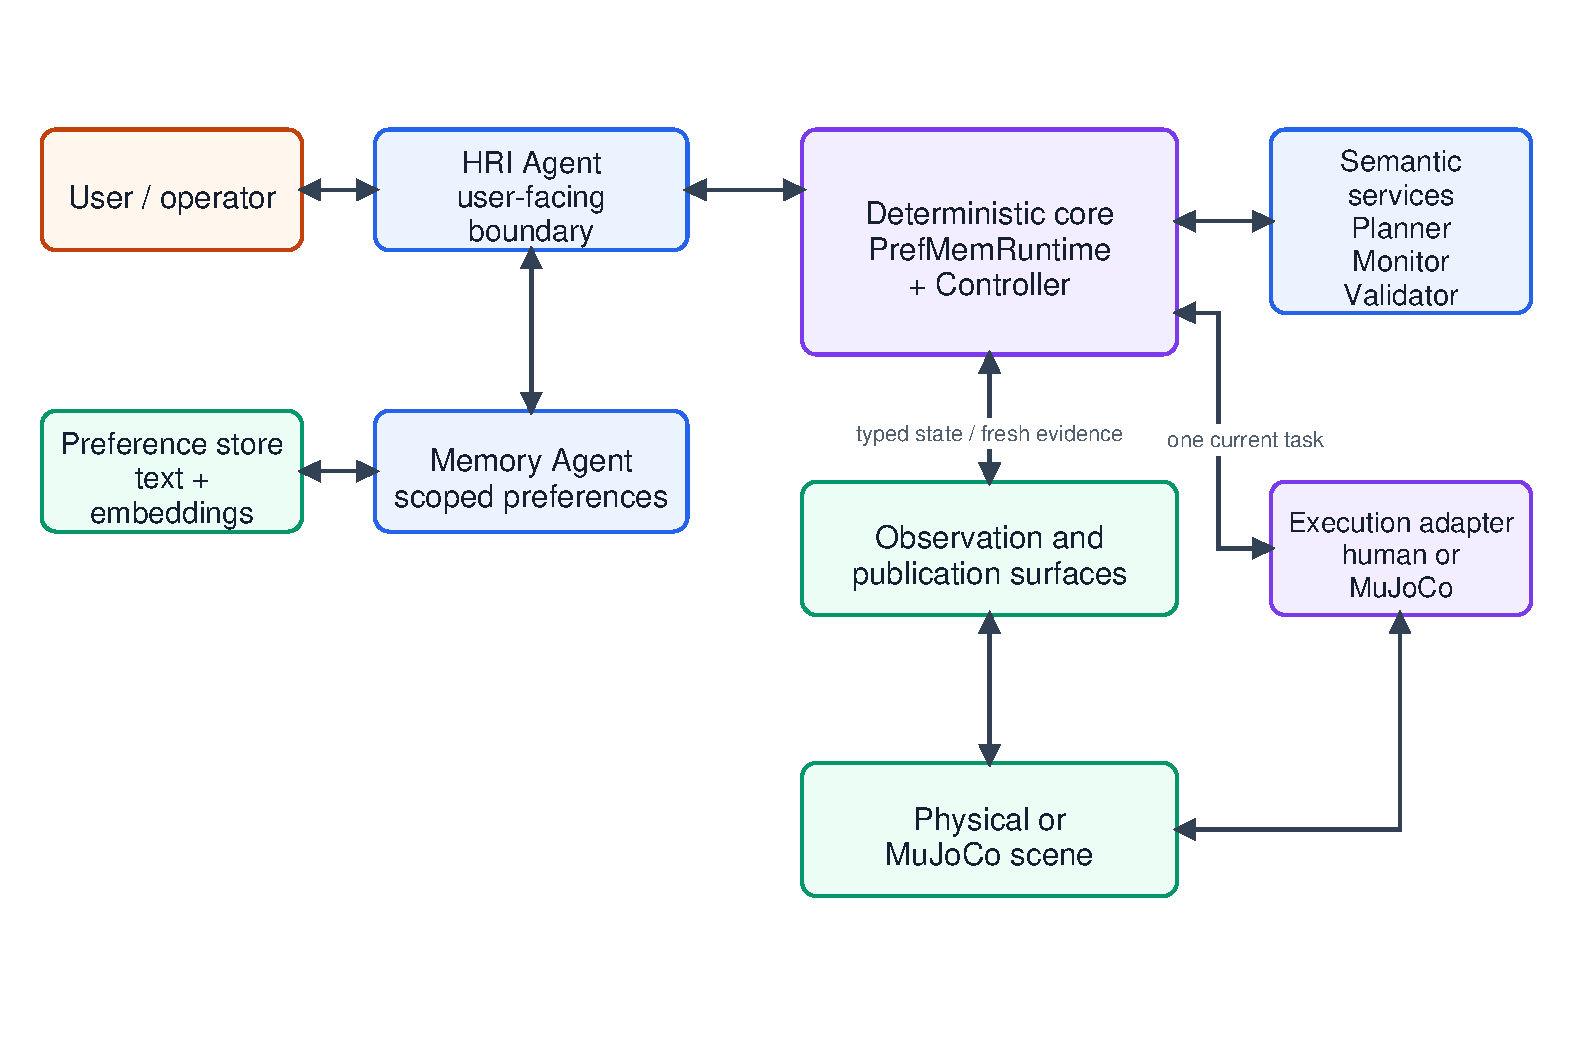
\includegraphics[width=0.92\textwidth]{figures/overall-architecture.pdf}
    \caption{Overall PrefMem component architecture. The semantic-services and
    execution-adapter blocks are expanded in the role-specific workflow
    subgraphs that follow. Blue nodes are model-facing roles, purple nodes are
    deterministic host components, green nodes are state or evidence surfaces,
    and orange nodes are human roles.}
    \label{fig:overall-architecture}
\end{figure}

Two deterministic components form the control plane. \texttt{PrefMemRuntime}
owns model and service composition, frame capture, task display publication,
observation-service routing, notifications, executor integration, and the
shared emergency coordinator. \texttt{RecedingHorizonController} owns the
frozen goal, cycle number, current publication, terminal history, evidence
streaks, attention reason, and loop guards. It performs no model calls and no
I/O; instead it returns explicit transitions for Runtime to execute.

The executor is connected through one \texttt{PublishedTask}. In human mode,
the current instruction is displayed through the camera-page task API. In
MuJoCo mode, the same publication is sent to \texttt{ExecutionService}. The
simulation atomically produces two synchronised observation streams. The
robot-hidden \texttt{sam} RGB-D view is reserved for grounding and execution,
whereas the third-person \texttt{prefmem} view preserves the visible robot for
HRI, Planner, Memory, Monitor, and Validator. This separation prevents semantic
agents from receiving simulator truth while allowing the executor to use
calibrated depth.

Persistent preference text is stored in \texttt{preference.json}, with
normalised EmbeddingGemma vectors in \texttt{preference.npy}. Terminal task
history is not stored in this preference database: it is immutable
controller-owned evidence scoped to one confirmed goal. The task publication
surface is likewise a single current slot rather than a queue, ensuring that a
human or robot sees only the authoritative active instruction.

\subsection{Deterministic Control Plane and Typed Contracts}
\label{subsec:methodology-contracts}

Figure~\ref{fig:controller-state-machine} gives the coarse controller state
graph. To keep the main graph legible, the active receding-horizon loop and its
exception handling are represented as components and expanded separately in
Figures~\ref{fig:controller-cycle-workflow}
and~\ref{fig:controller-exception-workflow}. A proposed goal moves the
controller from \texttt{IDLE} to \texttt{AWAITING\_CONFIRMATION}. Exact
confirmation starts the active loop. Planner can route to one executable step,
final validation, a blocker, or a user question. Stable terminal evidence
returns execution or incomplete validation to planning, while only stable
whole-goal validation can enter \texttt{COMPLETE}.

\begin{figure}[!htbp]
    \centering
    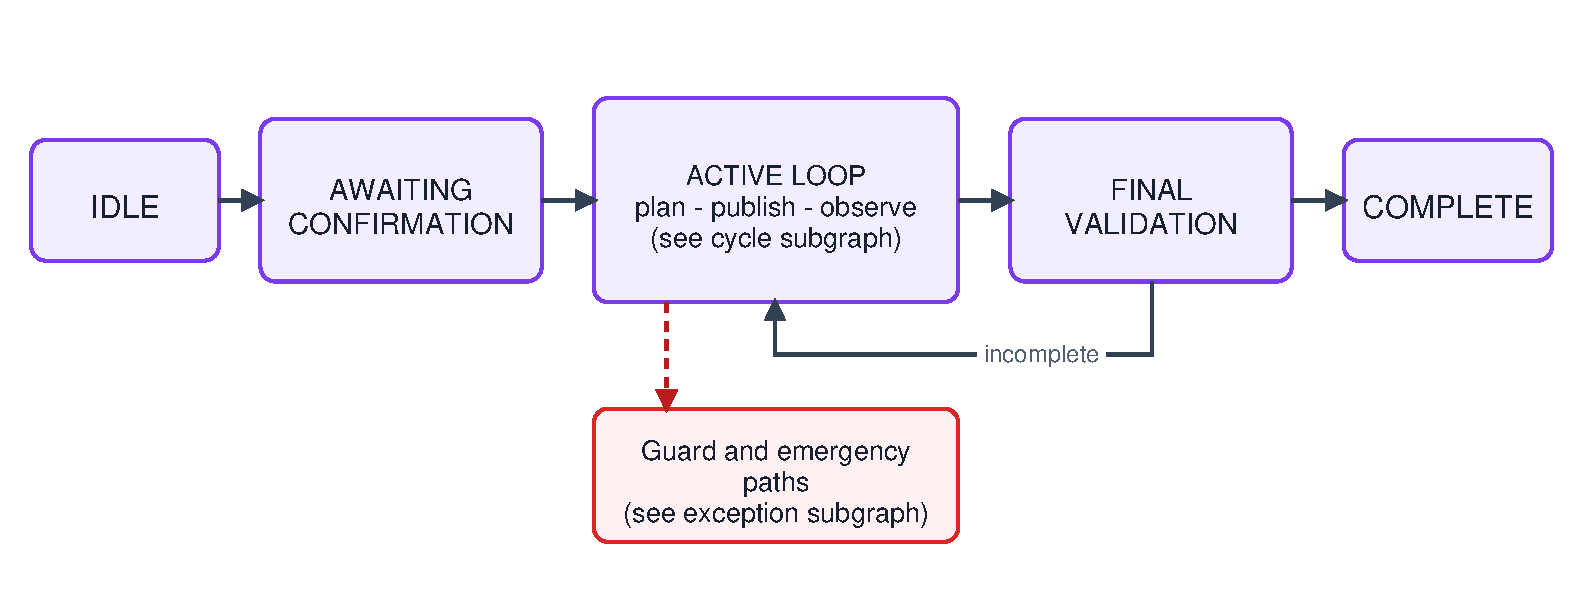
\includegraphics[width=0.90\textwidth]{figures/controller-state-machine.pdf}
    \caption{Top-level controller states. The active loop and guard paths are
    shown as components here and expanded in
    Figures~\ref{fig:controller-cycle-workflow}
    and~\ref{fig:controller-exception-workflow}.}
    \label{fig:controller-state-machine}
\end{figure}

\begin{figure}[!htbp]
    \centering
    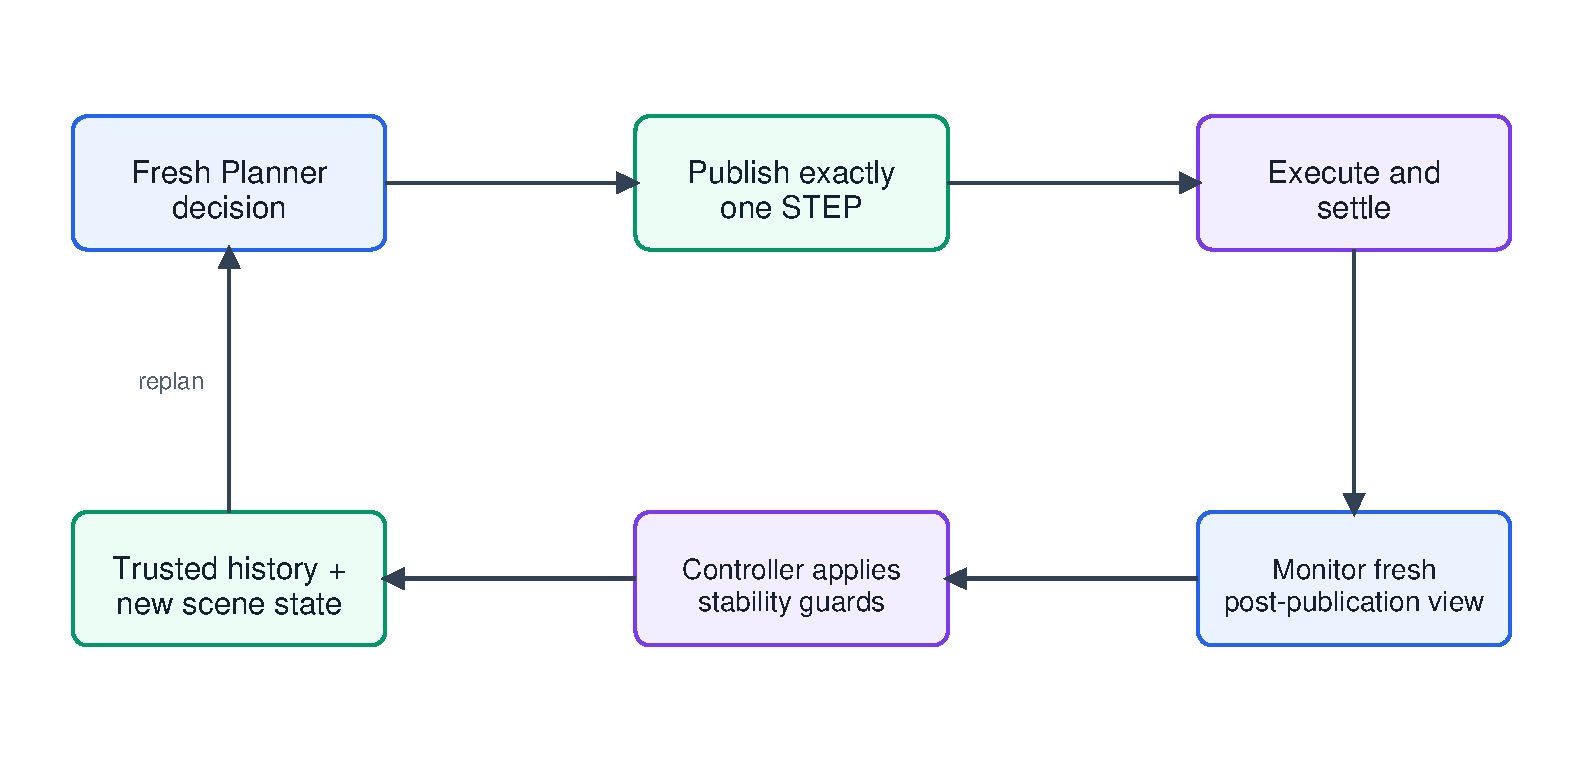
\includegraphics[width=0.90\textwidth]{figures/controller-cycle-workflow.pdf}
    \caption{Expanded active receding-horizon loop. Only one step is published;
    fresh post-publication evidence is converted into trusted history before
    the next Planner call.}
    \label{fig:controller-cycle-workflow}
\end{figure}

\begin{figure}[!htbp]
    \centering
    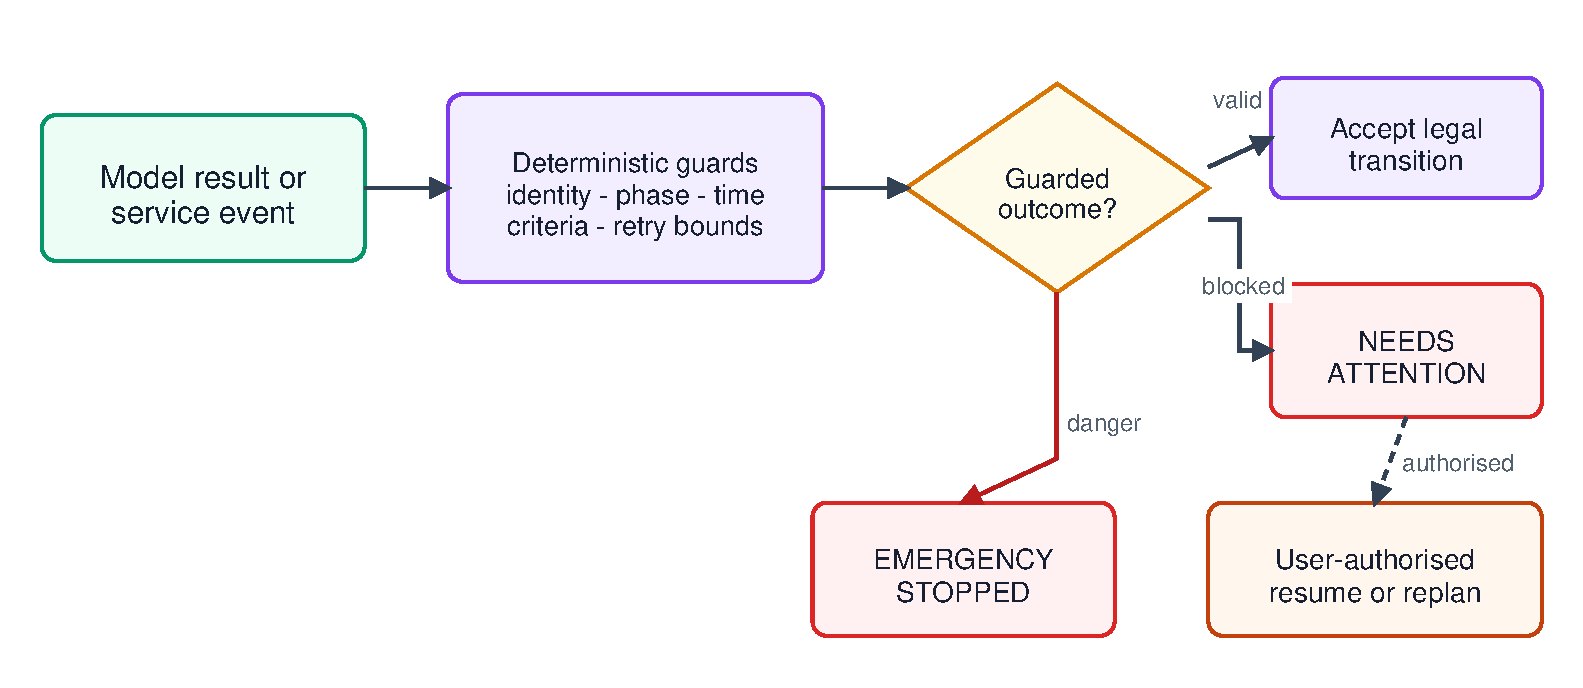
\includegraphics[width=0.90\textwidth]{figures/controller-exception-workflow.pdf}
    \caption{Expanded controller guard and exception routing. Invalid or
    exhausted operations enter \texttt{NEEDS\_ATTENTION}; valid danger evidence
    enters the process-terminal \texttt{EMERGENCY\_STOPPED} state.}
    \label{fig:controller-exception-workflow}
\end{figure}

Typed contracts make graph edges executable and auditable. A
\texttt{GoalProposal} contains the scene-grounded proposed outcome, explicit
constraints, nominal outline, and observable final state. Runtime converts a
non-blocked proposal into a \texttt{GoalContract} with a trusted goal identifier
and revision. A \texttt{ValidationContract} maps each broad final outcome to
detailed visual criteria and is frozen at confirmation. A
\texttt{PlannerCycleRequest} binds the immutable goal to a fresh frame, trigger,
trusted terminal history, and optional operator guidance.

For an action decision, host code selects only
\texttt{candidate\_tasks[0]} and constructs a \texttt{PublishedTask} with trusted
cycle, step, criterion, publication, phase, and timestamp fields. Monitor and
Validator responses are parsed into typed assessments and rejected if their
identifiers, ordered criterion set, frame sequence, or phase do not match
authoritative state. Only deterministic transitions append an
\texttt{ExecutionRecord}, request another planning cycle, enter attention, or
establish completion. This implements the rule that models may propose
semantics, but host code owns lifecycle state.

\newpage

\subsection{HRI Agent Design}
\label{subsec:methodology-hri}

\paragraph{Responsibility and inputs.}
HRI is the only role permitted to converse with the user. Each model call
receives the current user message, a current \texttt{prefmem} frame,
conversation messages, and an injected authoritative runtime summary. That
summary exposes the staged or confirmed goal, current publication, terminal
history, validation report, attention cause, and currently authorised recovery
actions. Conversation history helps interpret the current turn but is not
authoritative state and does not by itself authorise a new preference.

\paragraph{Tool surface and authority.}
Once Runtime is attached, the generic sub-agent tool is replaced by five
strictly typed tools: call Memory, request a goal preview, confirm an exact goal
revision, resume the current publication, or request replanning with optional
guidance. Planner cycles, publication, Monitor/Validator control, history
mutation, and emergency reset are deliberately absent. Tool errors are returned
as structured observations so the dialogue can report them without bypassing
the control plane; a latched emergency disables further tool execution.

\paragraph{Workflow.}
Figures~\ref{fig:hri-workflow} and~\ref{fig:hri-confirmation-workflow} separate
the HRI loop into intent resolution and contract confirmation. HRI first
determines whether the physical outcome and important constraints are
sufficiently clear. For an under-specified reference, it requests Memory before
guessing. One applicable non-conflicting preference may fill the missing field;
empty, irrelevant, or conflicting evidence produces one focused clarification.

\begin{figure}[!htbp]
    \centering
    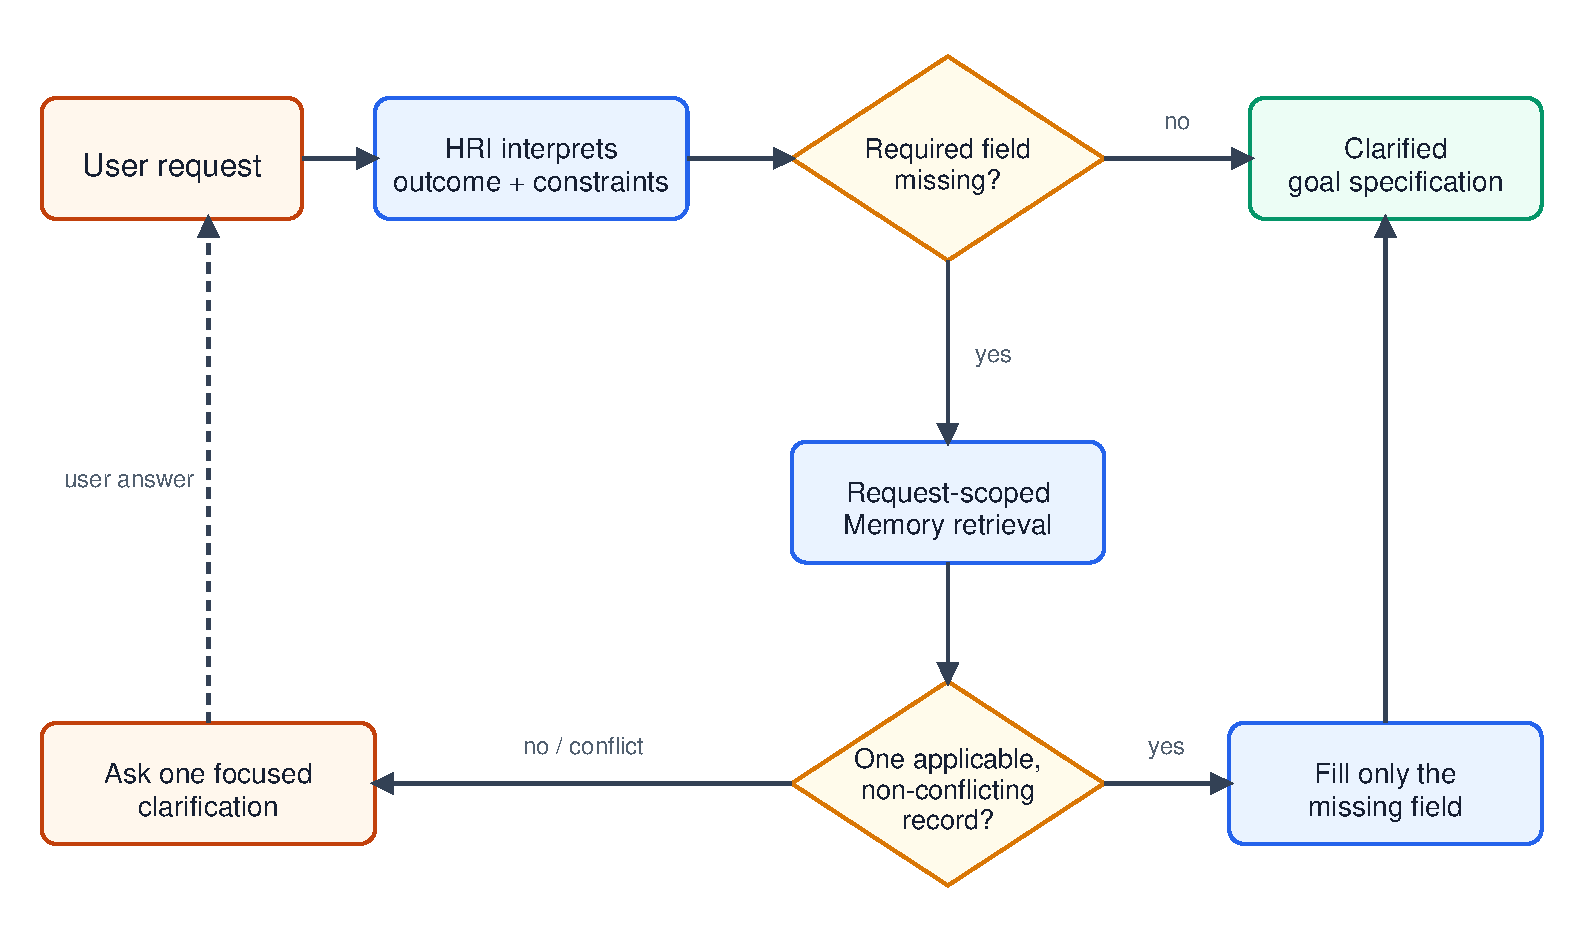
\includegraphics[width=0.90\textwidth]{figures/hri-workflow.pdf}
    \caption{HRI intent-resolution subgraph. Memory may supply only a missing
    field when one applicable non-conflicting record exists; otherwise HRI asks
    one focused clarification.}
    \label{fig:hri-workflow}
\end{figure}

Once the request is clear, HRI asks Runtime for a scene-grounded preview and
presents the exact goal, constraints, expected outcomes, nominal strategy, goal
identifier, and revision. It may invoke confirmation only after the user refers
to that exact identity. Rejection retains the proposal for discussion but
authorises no execution.

\begin{figure}[!htbp]
    \centering
    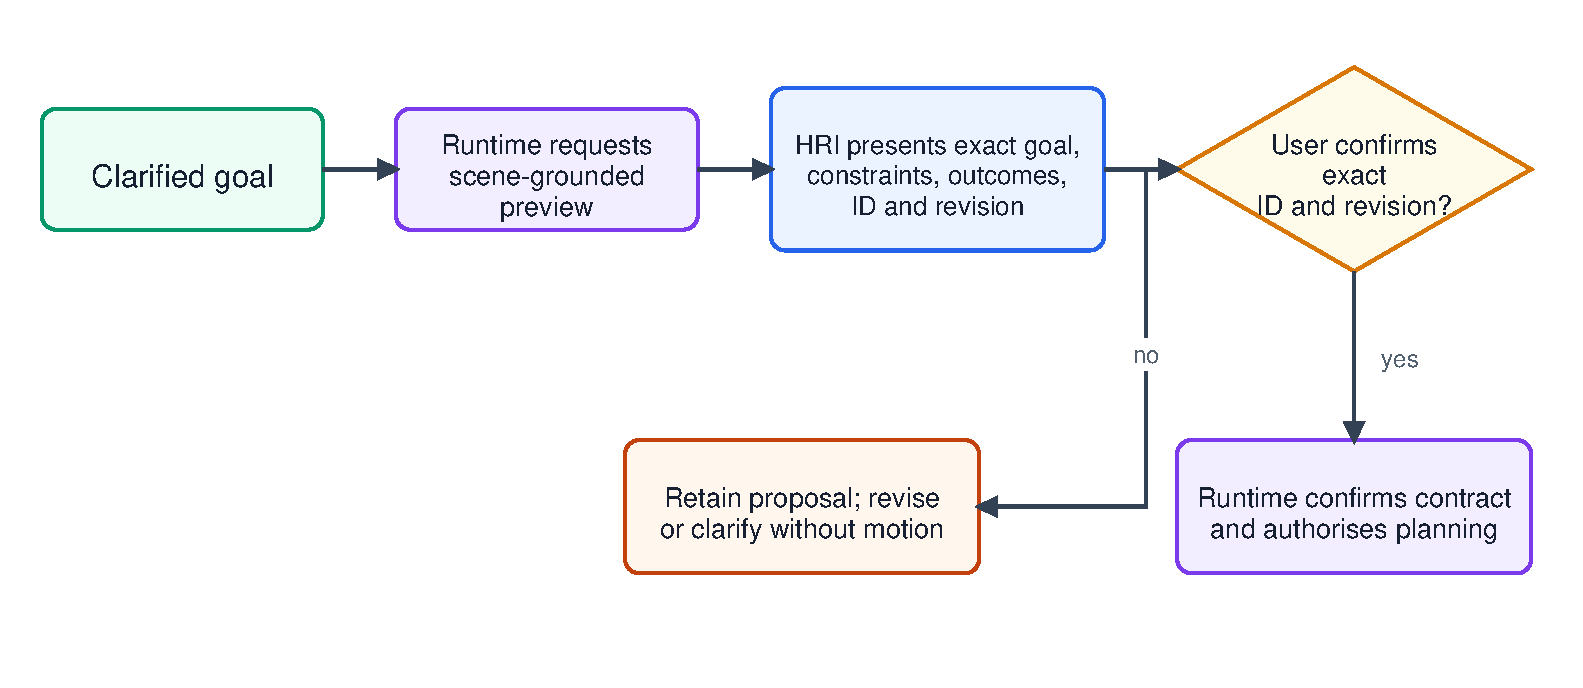
\includegraphics[width=0.90\textwidth]{figures/hri-confirmation-workflow.pdf}
    \caption{HRI preview-and-confirmation subgraph. The HRI model presents the
    contract, while Runtime alone validates the exact goal identity and permits
    planning.}
    \label{fig:hri-confirmation-workflow}
\end{figure}

HRI also translates controller notifications into a user-facing report. On
completion it exposes the broad frozen checklist rather than internal detailed
criteria; on attention it reports the authoritative cause and only the recovery
actions currently legal. The HRI/Memory/contract boundary is evaluated by the
HRI component and interface studies and by focused EXP-01 through EXP-05. These
experiments test the combined decision boundary rather than proving universal
natural-language understanding.

\subsection{Memory Agent Design}
\label{subsec:methodology-memory}

\paragraph{Store and request boundary.}
Memory maintains a list of preference records and a row-aligned matrix of
normalised embeddings. Requests must begin with \texttt{RETRIEVE REQUEST:} or
\texttt{MUTATE REQUEST:}. Each request receives a new request identifier and
isolated graph thread, clearing prior retrieval evidence so that an earlier
tool trace cannot authorise a later write. The Memory model has four tools:
retrieve, remember, update, and forget. Its graph alternates between one model
node and a tool node until the model returns a final JSON response.

\paragraph{Two-stage retrieval.}
As illustrated in Figure~\ref{fig:memory-workflow}, the model first generates
focused query phrasing. EmbeddingGemma encodes each query; cosine similarity is
computed against the normalised store. Each query contributes its configured
top-\(k\) candidates. Host code then applies deterministic ranking,
deduplication by memory identifier, maximum-similarity merging, and a global
cap. The current measured configuration uses \(k=3\) and cap \(=3\). The
semantic model receives only this bounded set and may return only unchanged
records whose identifiers, text, and similarity match the candidates. This
separates high-recall candidate construction from task-specific applicability
judgement.

\begin{figure}[!htbp]
    \centering
    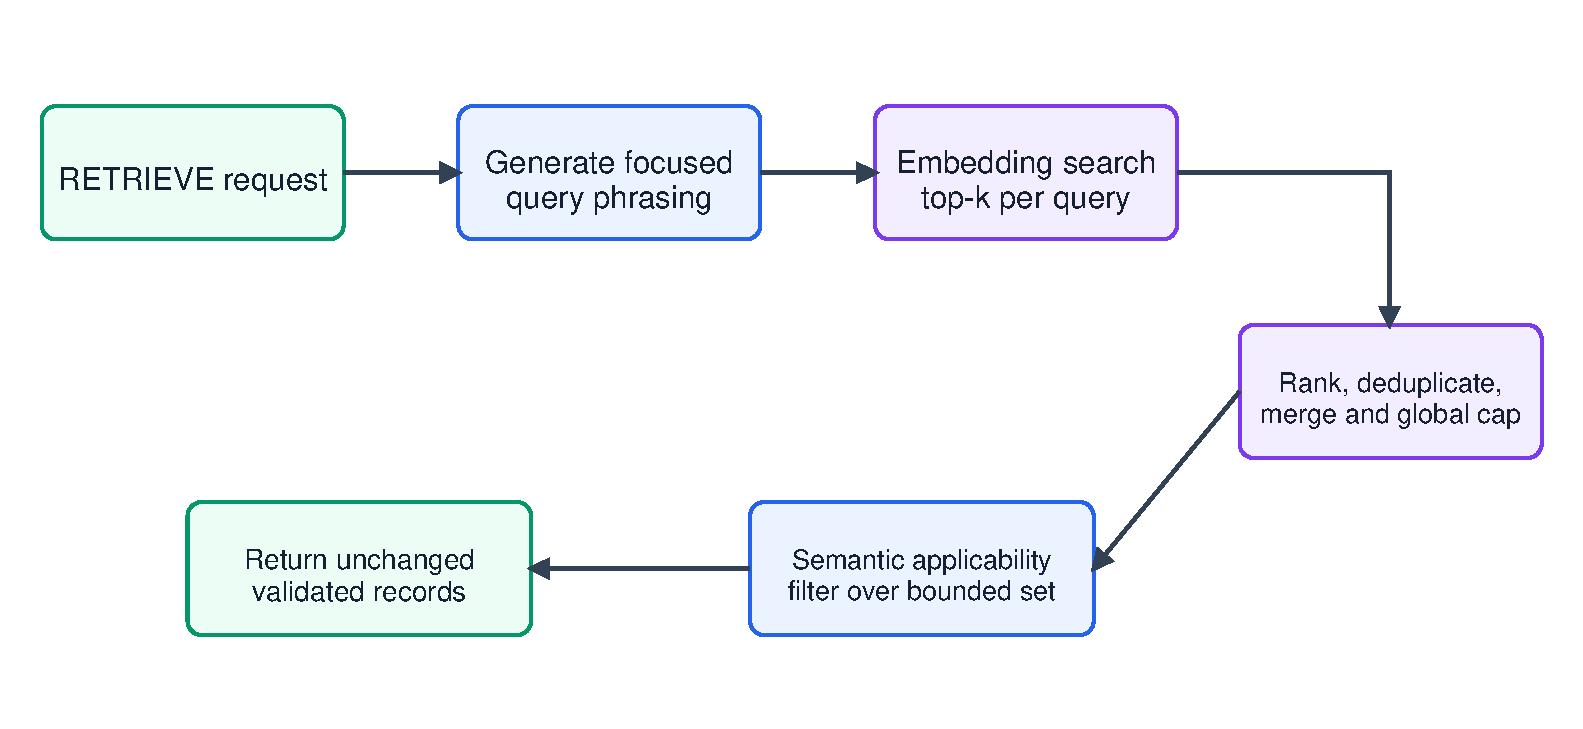
\includegraphics[width=0.90\textwidth]{figures/memory-workflow.pdf}
    \caption{Memory retrieval subgraph. Deterministic candidate construction
    bounds the records passed to the semantic applicability filter.}
    \label{fig:memory-workflow}
\end{figure}

\paragraph{Mutation policy.}
A write tool is invalid unless the current request is labelled as mutation and
retrieval has already occurred. Update and forget targets must be among the
records retrieved for that same request. The model may perform at most one
justified remember, update, or forget operation; otherwise it returns a no-op or
error. HRI separately enforces the future-facing consent policy: exact
confirmation of the current physical goal is not memory consent. Text records
and their regenerated embeddings are persisted together as the preference
store, and optional trace sinks record queries, scores, caps, returned IDs, and
timing without changing the response.

\begin{figure}[!htbp]
    \centering
    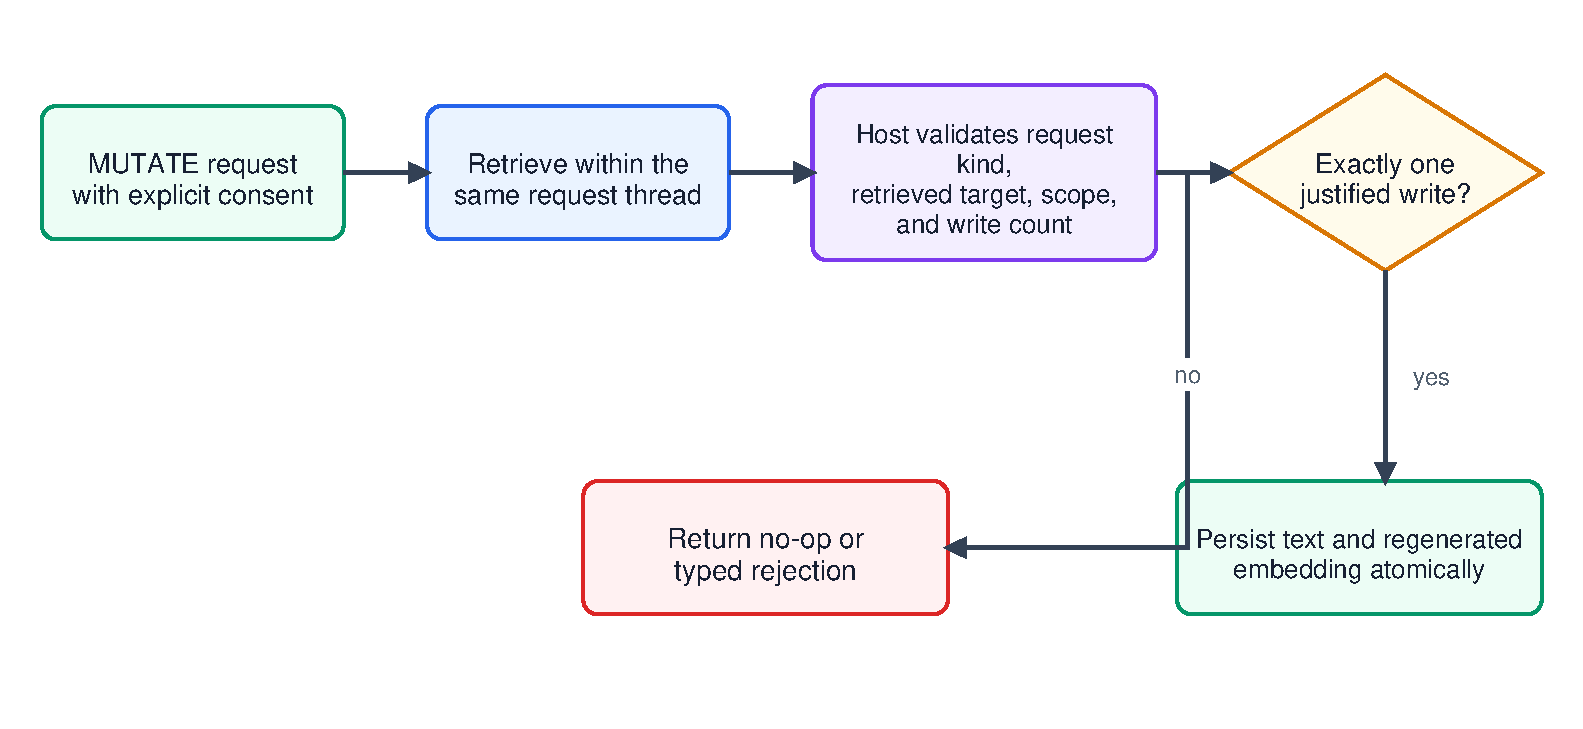
\includegraphics[width=0.90\textwidth]{figures/memory-mutation-workflow.pdf}
    \caption{Memory mutation subgraph. Retrieval must occur within the same
    isolated request before host code permits at most one justified write.}
    \label{fig:memory-mutation-workflow}
\end{figure}

The design nevertheless relies on free-text records and model-mediated
mutation identity. The longitudinal experiment tests creation, immediate use,
update, delayed retrieval, scope isolation, and revocation and exposes cases in
which semantically related writes can target the wrong identity. This is a
measured limitation and motivates future structured user, task, and preference-
dimension keys.

\subsection{Planner Agent Design}
\label{subsec:methodology-planner}

Planner is a stateless, scene-grounded VLM boundary with two typed modes. It has
no tools, persistent conversation, publication authority, or mutable plan
queue. Every call contains a system prompt, one current image, and one explicit
request payload. Temperature is zero, and returned text must parse into the
requested contract; invalid shapes receive only a bounded targeted schema-
correction attempt before Runtime treats the call as an error.

\paragraph{Preview mode.}
Before confirmation, Planner receives the clarified goal, explicit constraints,
optional guidance, and a fresh frame. It returns a \texttt{GoalProposal} whose
status is \texttt{READY}, \texttt{ALREADY\_SATISFIED}, or \texttt{BLOCKED}. A
ready proposal includes the exact high-level outcome, constraints, observable
final results, and a short nominal outline. The outline communicates strategy
to the user but is neither frozen nor executable. Runtime, not Planner, assigns
the goal identifier and revision.

\begin{figure}[!htbp]
    \centering
    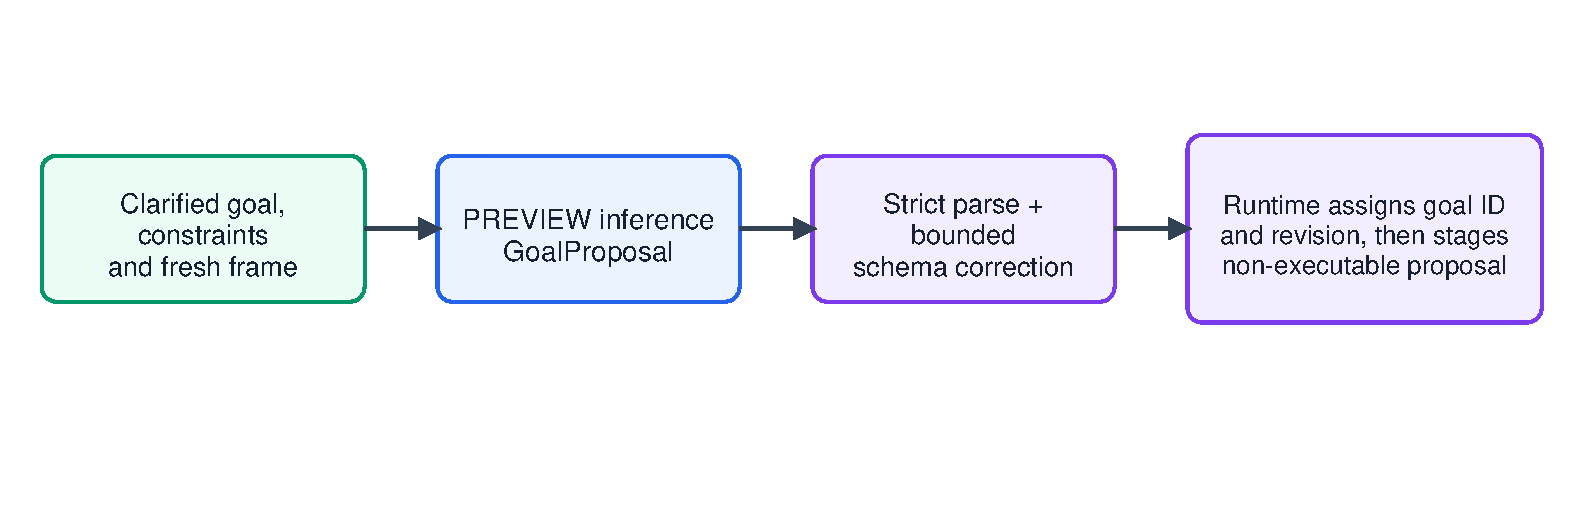
\includegraphics[width=0.90\textwidth]{figures/planner-workflow.pdf}
    \caption{Planner preview subgraph. The returned outline is non-executable;
    Runtime parses it and assigns the trusted goal identity.}
    \label{fig:planner-preview-workflow}
\end{figure}

\paragraph{Execution-cycle mode.}
After confirmation, Planner receives the immutable \texttt{GoalContract}, a
strictly fresh frame, the cycle trigger, ordered terminal history, and optional
operator guidance. It returns \texttt{ACT},
\texttt{REQUEST\_FINAL\_VALIDATION}, \texttt{BLOCKED}, or
\texttt{NEEDS\_USER\_INPUT}. An action may contain up to three candidate tasks,
but the controller publishes only the first and discards the prediction tail.
The next call therefore reasons from the scene actually produced by execution
rather than continuing a stale predicted queue. Figure~\ref{fig:planner-cycle-workflow}
shows this execution-cycle boundary separately from preview.

\begin{figure}[!htbp]
    \centering
    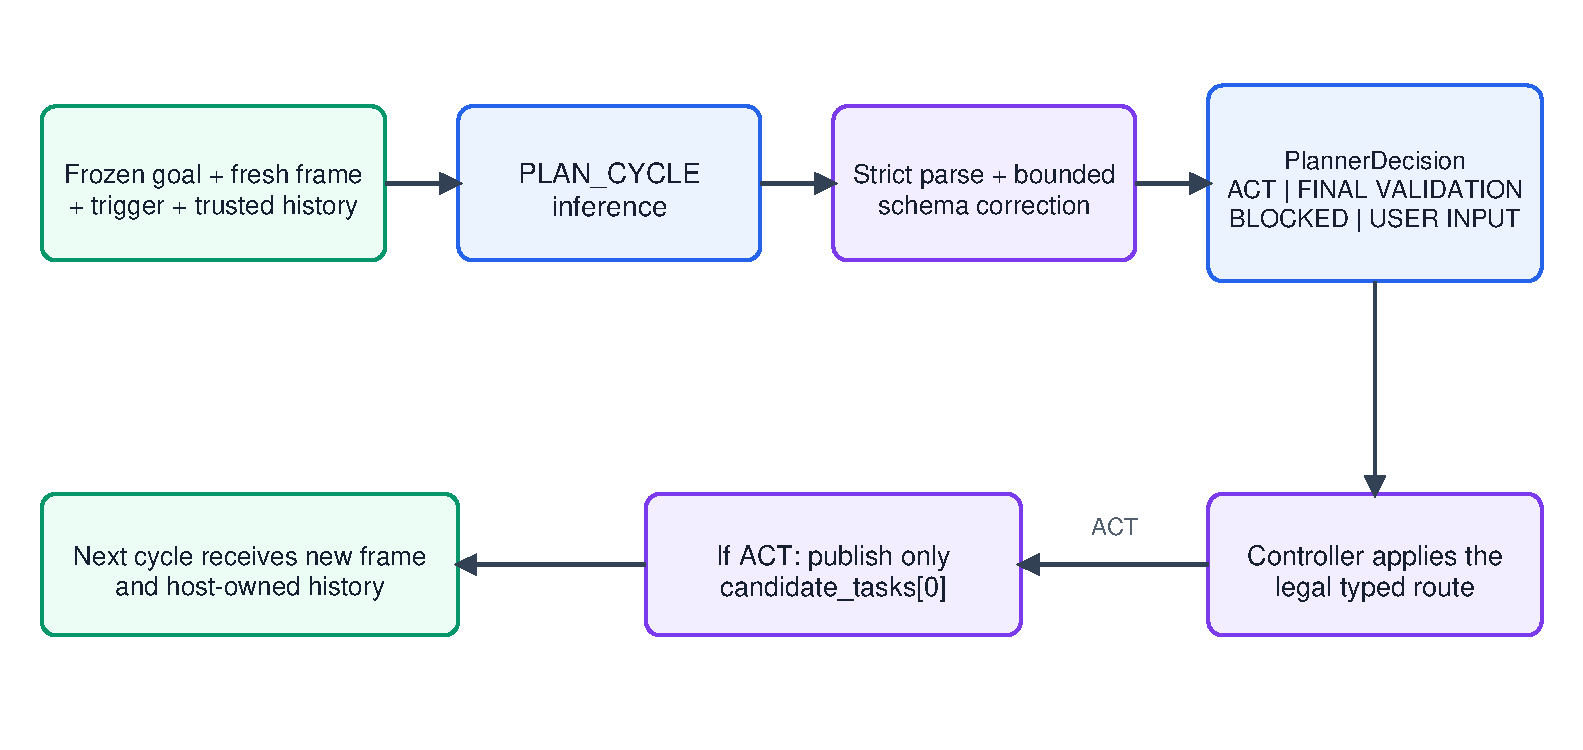
\includegraphics[width=0.90\textwidth]{figures/planner-cycle-workflow.pdf}
    \caption{Planner execution-cycle subgraph. Planner proposes a typed route;
    Controller applies it and, for \texttt{ACT}, publishes only the first
    candidate before collecting a fresh frame and trusted history.}
    \label{fig:planner-cycle-workflow}
\end{figure}

Planner cannot weaken the goal after failure, mark execution complete, or infer
success from the number of attempted actions. It sees Monitor and Validator
outputs only after Controller has converted them into trusted history. Its
fresh-frame, history-use, grounding, capability-fence, and completion-routing
behaviour are evaluated by the Planner component studies, named interfaces,
workflow ladder, and replanning ablations. Deterministic replanning ablations
justify the control policy but are not evidence of learned Planner quality.

\subsection{Monitor Agent Design}
\label{subsec:methodology-monitor}

Monitor is an asynchronous observation service for exactly one active
\texttt{STEP} publication. Publishing a task increments a service generation,
replaces the single active slot, and starts the worker if necessary. The worker
captures the latest \texttt{prefmem} frame at a bounded interval and begins no
inference unless its timestamp and frame sequence are newer than the
publication. Replacing or retiring the task invalidates the generation, so a
late callback cannot mutate the replacement publication.

The model prompt contains the publication, frozen goal identity and revision,
step ID, instruction, ordered expected-observation criteria, and known failure
conditions. It returns criterion states, a grounded observation, overall
\texttt{ONGOING}, \texttt{SUCCESS}, or \texttt{FAIL}, an optional failure
report, and an emergency envelope. Host parsing requires the exact ordered
criterion IDs. A camera, model, parser, or callback error is reported as a
service error and retires the observation job; it is never relabelled as a
physical task failure.

\begin{figure}[!htbp]
    \centering
    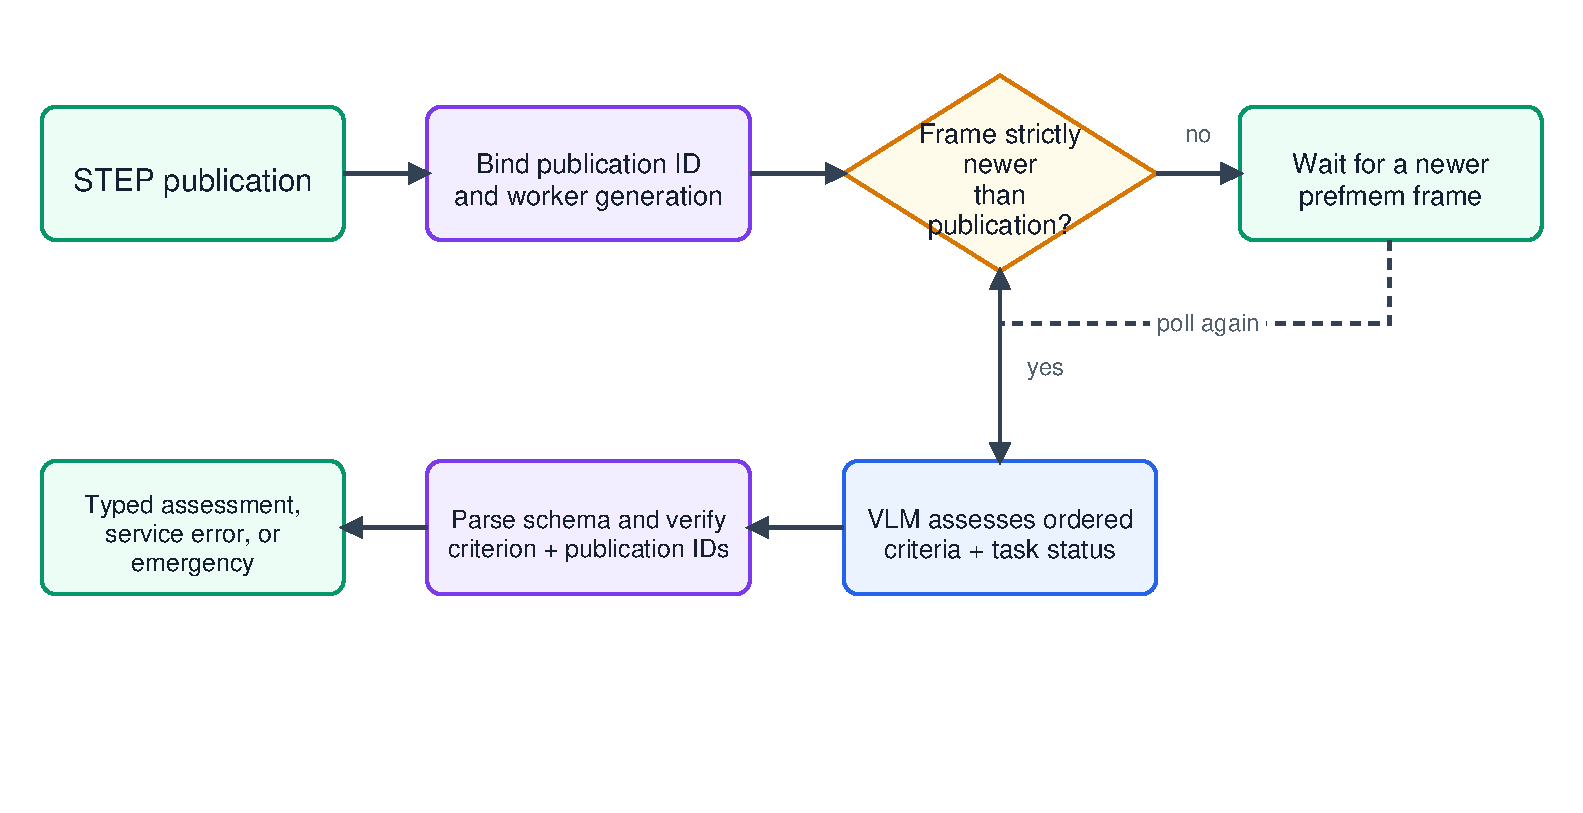
\includegraphics[width=0.90\textwidth]{figures/monitor-workflow.pdf}
    \caption{Monitor observation-service subgraph. The learned assessment runs
    only on a frame that is strictly newer than the bound publication.}
    \label{fig:monitor-workflow}
\end{figure}

A valid emergency envelope bypasses ordinary task-result parsing so visible
danger cannot be hidden by an in-flight replacement. Otherwise Runtime accepts
only an assessment that still belongs to the active publication. Controller
then applies deterministic temporal aggregation. By default, success requires
two confirmations spanning at least two seconds and failure requires two
confirmations. An increase in the number of met criteria refreshes the
no-progress clock; an inconclusive view does not itself erase prior candidate
success unless a visible contradiction appears. In MuJoCo mode, terminal
Monitor evidence is deferred until the executor reports that motion has
settled.

\begin{figure}[!htbp]
    \centering
    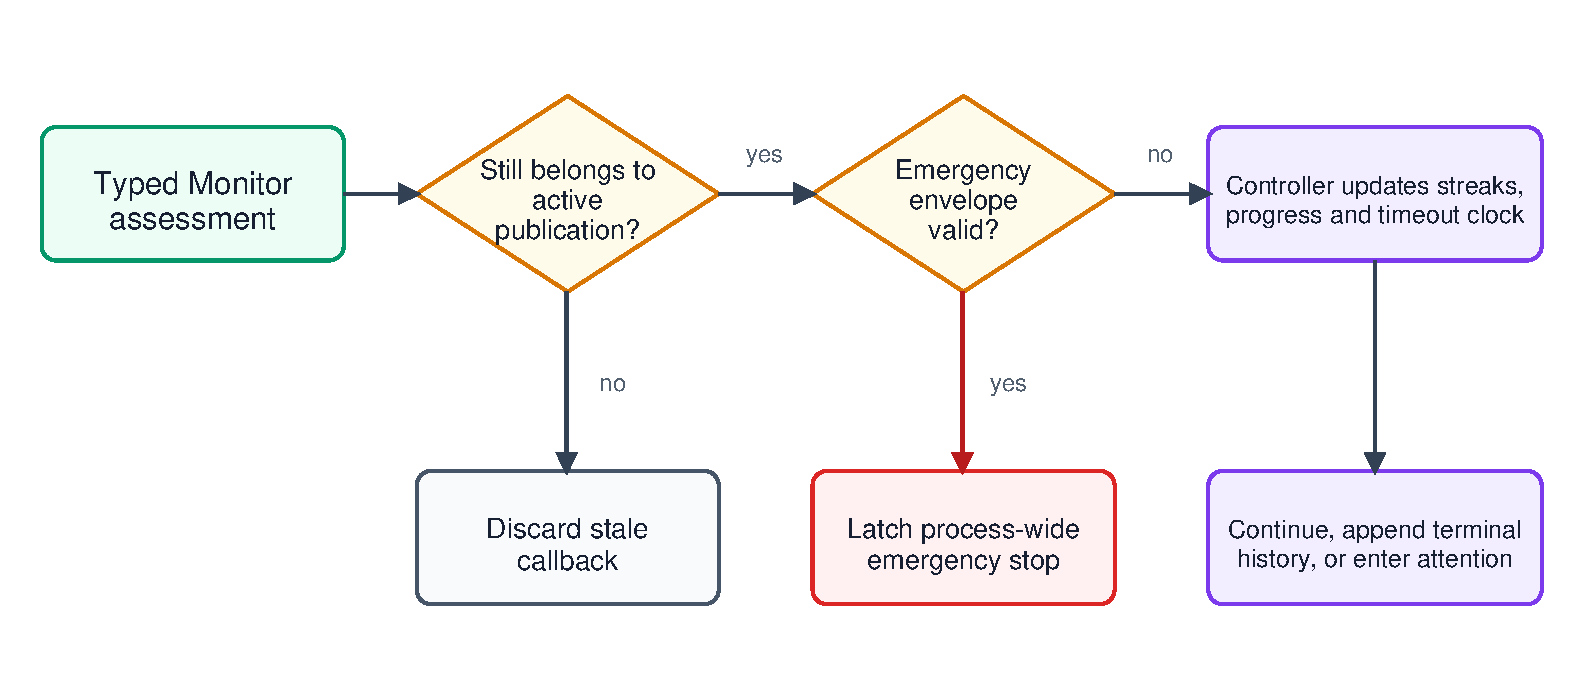
\includegraphics[width=0.90\textwidth]{figures/monitor-aggregation-workflow.pdf}
    \caption{Monitor host-aggregation subgraph. Runtime rejects stale callbacks
    or latches valid emergency evidence before Controller updates progress and
    terminal-stability state.}
    \label{fig:monitor-aggregation-workflow}
\end{figure}

Monitor is deliberately not the whole-goal authority. It determines whether
the current instruction appears ongoing, successful, or failed. The component
and interface studies test classification, temporal stability, progress,
errors, stale events, and Planner hand-off, while EXP-06 compares production
Monitor with a no-visual-advancement control. These results must separate
learned visual recognition from deterministic host timing and fencing.

\subsection{Validator Agent Design}
\label{subsec:methodology-validation}

Validator implements two workflows around one immutable
\texttt{ValidationContract}. During exact confirmation, it receives the
\texttt{GoalContract} and confirmation frame and expands every broad final
outcome into ordered detailed visible criteria. Contract construction validates
that each detailed criterion maps to exactly one broad outcome and that every
broad outcome is covered. Compilation must finish before planning is
authorised. The resulting checklist is frozen with the goal so later failure
cannot weaken the definition of success.

\begin{figure}[!htbp]
    \centering
    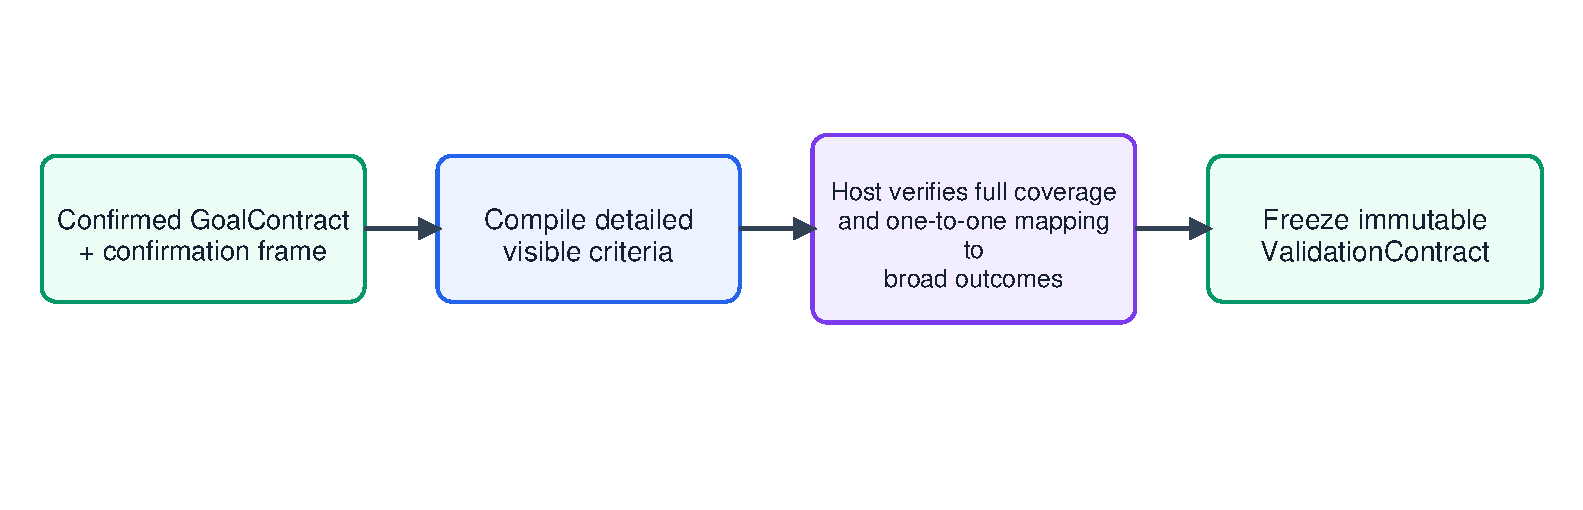
\includegraphics[width=0.90\textwidth]{figures/validator-workflow.pdf}
    \caption{Validator checklist-compilation subgraph. Host validation requires
    complete coverage before freezing the immutable validation contract.}
    \label{fig:validator-contract-workflow}
\end{figure}

During execution, Planner may request final validation. Controller then creates
a \texttt{FINAL\_VALIDATION} publication instructing the operator to leave
objects unchanged and move only the camera when needed. The Validator service
accepts only a publication whose goal ID and revision match the frozen
contract. Like Monitor, it polls strictly post-publication \texttt{prefmem}
frames, fences service generations, and treats model/schema errors separately
from physical incompleteness.

\begin{figure}[!htbp]
    \centering
    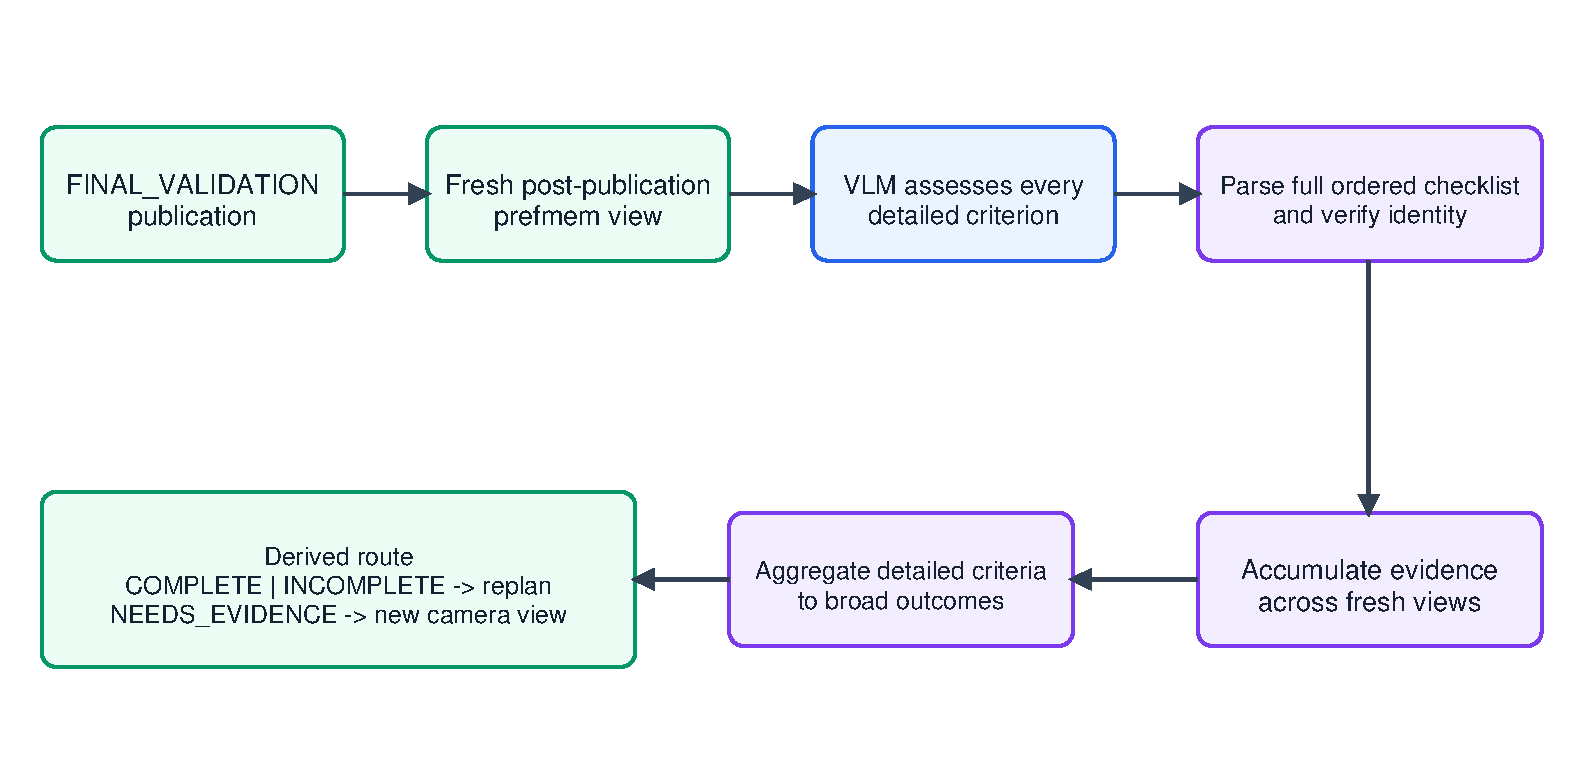
\includegraphics[width=0.90\textwidth]{figures/validator-assessment-workflow.pdf}
    \caption{Validator final-assessment subgraph. Host code verifies the full
    ordered checklist, accumulates evidence across fresh views, and derives the
    final route from the frozen broad outcomes.}
    \label{fig:validator-assessment-workflow}
\end{figure}

Each assessment must cover the complete ordered detailed checklist. The service
accumulates evidence across views: a later \texttt{MET} or \texttt{NOT\_MET}
can replace an earlier \texttt{UNKNOWN}, while a new unknown view does not erase
previously visible evidence. Runtime converts the accumulated assessment into a
\texttt{ValidationReport}. Host aggregation maps detailed criteria back to the
frozen broad outcomes and deterministically derives \texttt{COMPLETE},
\texttt{INCOMPLETE}, or \texttt{NEEDS\_EVIDENCE}. Unknown evidence requests
camera movement only; it does not prove a task failure. Stable incomplete
evidence becomes a
\texttt{FINAL\_\allowbreak{}VALIDATION\_\allowbreak{}FAIL} history record and returns
to planning. Stable complete evidence is the only ordinary path to
\texttt{COMPLETE}.

Validator is independent in responsibility and context, not in model weights:
it currently shares the primary Gemma endpoint with the other semantic roles.
The separate frozen checklist and host aggregation prevent Planner from
certifying its own task count, but correlated visual errors remain possible.
Validator component studies test checklist coverage, final-state judgement,
history use, missing evidence, and reset isolation; EXP-07 tests false-
completion prevention, and EXP-09 exposes the cost of false rejection in a
dynamic low-contrast case.

\subsection{Execution Adapter Design}
\label{subsec:methodology-executor}

The executor is deliberately narrower than the task-level agents. It accepts
only a current \texttt{STEP} publication and exposes no goal-revision,
preference, confirmation, or completion authority. In human mode the adapter is
the task display and a person performs the instruction. In MuJoCo mode,
\texttt{ExecutionService} owns one asynchronous publication-fenced job and
passes it through compilation, grounding, control, settling, and outcome
recording. Figure~\ref{fig:executor-workflow} shows the strict execution path;
Figure~\ref{fig:executor-assistance-workflow} isolates the experiment-only
assistance path so it cannot be mistaken for ordinary execution.

\begin{figure}[!htbp]
    \centering
    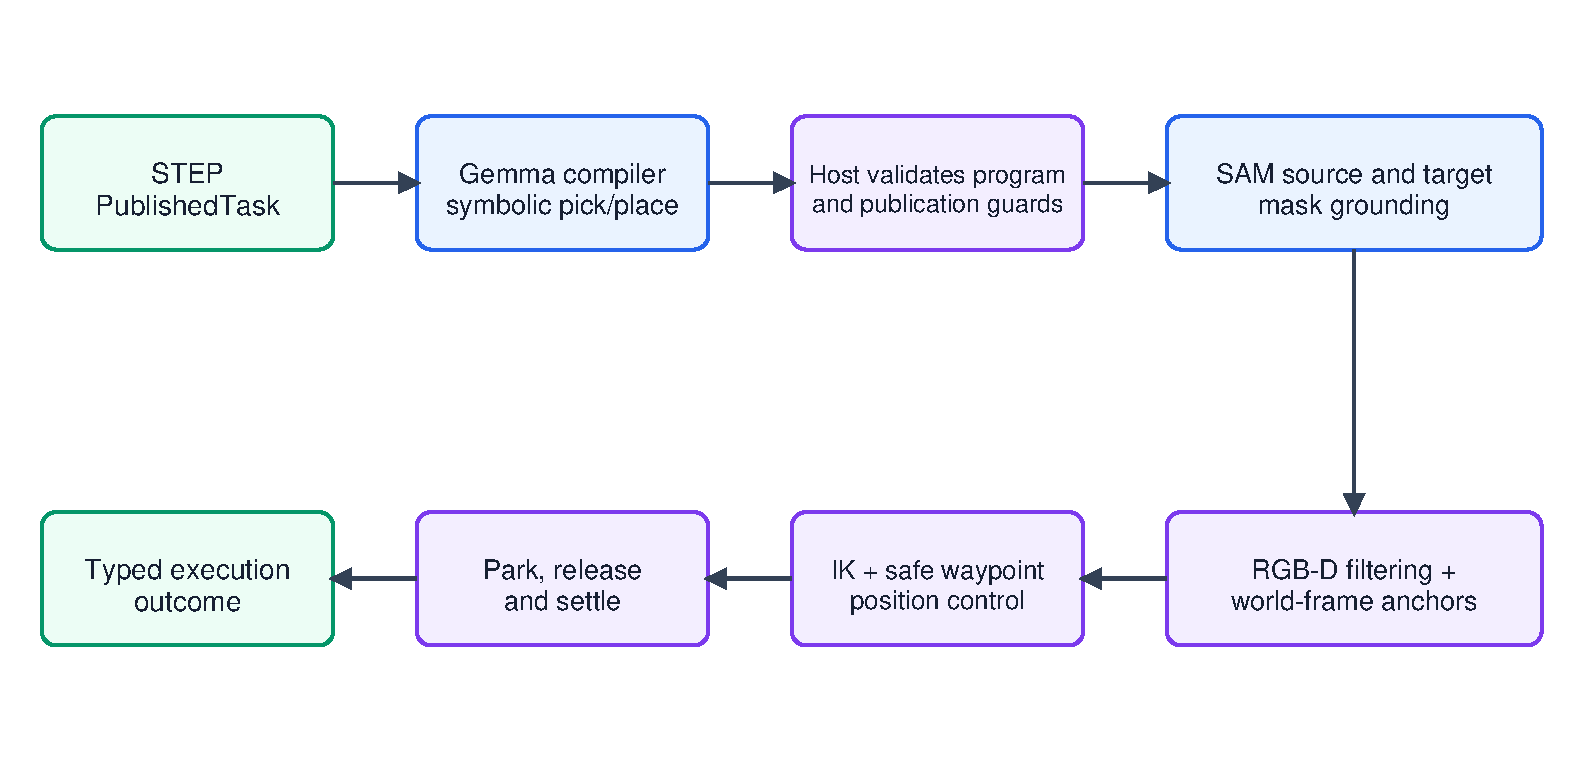
\includegraphics[width=0.90\textwidth]{figures/executor-workflow.pdf}
    \caption{Strict MuJoCo execution-adapter subgraph from publication through
    compilation, grounding, deterministic control, settling, and typed outcome.}
    \label{fig:executor-workflow}
\end{figure}

Gemma 4 compiles the natural-language instruction into a strict supported
pick/place program. Host validation rejects unsupported operations, malformed
selectors, and invalid anchors before motion. SAM 3.1 receives the robot-hidden
\texttt{sam} image and returns source and target masks. Synchronized depth,
calibrated intrinsics, and camera extrinsics convert filtered mask points into
world-frame anchors. A damped-least-squares IK and position controller then
executes a fixed safe waypoint sequence for approach, grasp, lift, transfer,
place, release, retreat, and parking. Runtime treats executor activity as a
liveness heartbeat but not as visual proof that the task criterion is met.
After motion, the robot is parked and the manipulated object is allowed to
settle before Monitor can establish a terminal result.

Cancellation and scene-change requests route the controller to a safe hold
before replanning. Experiments may explicitly enable simulator-oracle grounding
after a typed post-call grounding failure. The strict SAM attempt and the
assisted downstream continuation remain separately recorded; an empty, wrong,
or service-invalid grounding is not silently corrected. Calibration,
\texttt{C-EXE}, EXP-08, and EXP-09 decompose compiler, mask, anchor, motion, and
end-to-end behaviour. The adapter is supporting infrastructure and must not be
described as a learned VLA contribution.

\begin{figure}[!htbp]
    \centering
    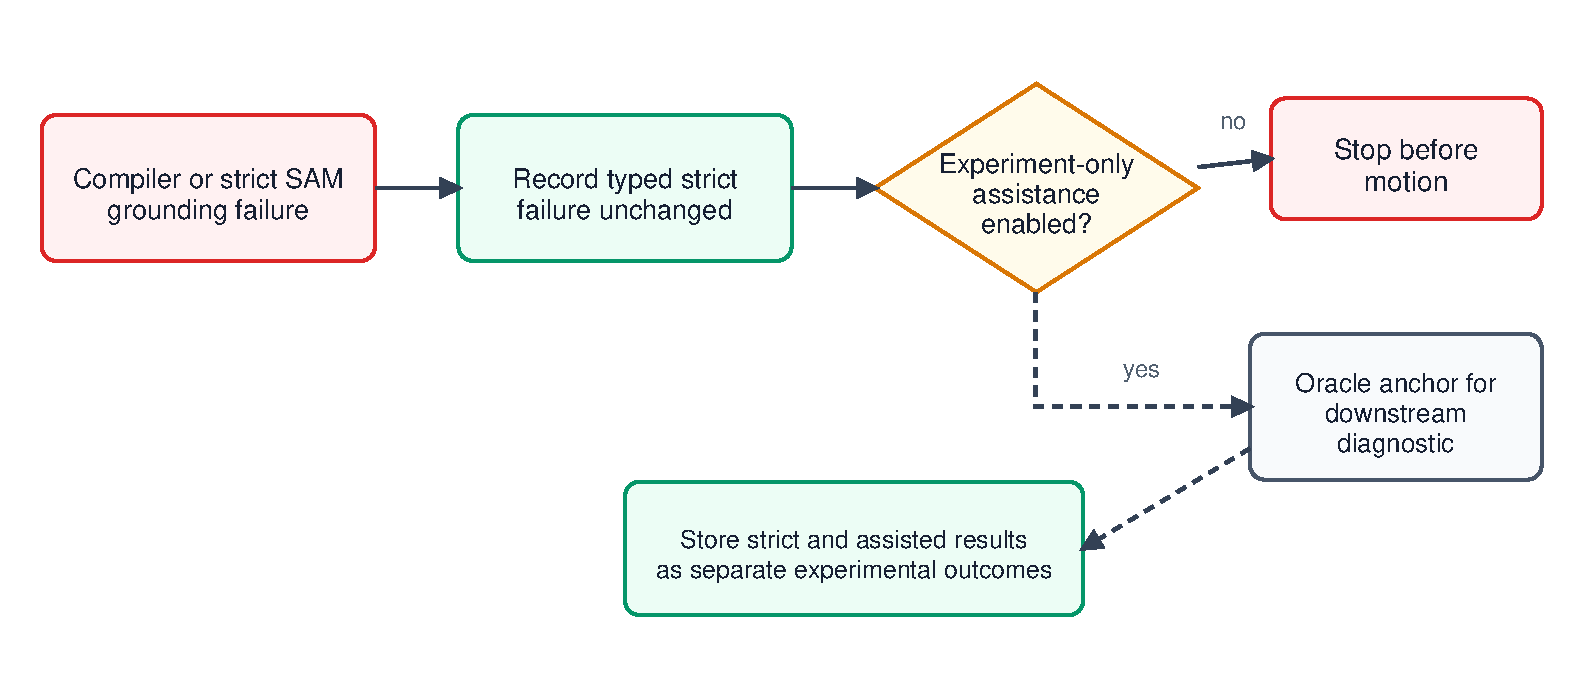
\includegraphics[width=0.90\textwidth]{figures/executor-assistance-workflow.pdf}
    \caption{Experiment-only grounding-assistance subgraph. The strict failure
    remains recorded even when an oracle anchor permits a separate downstream
    diagnostic continuation.}
    \label{fig:executor-assistance-workflow}
\end{figure}

\subsection{Inter-Agent Interaction Protocol}
\label{subsec:methodology-interactions}

The agents do not participate in an unrestricted shared conversation.
Figure~\ref{fig:interaction-protocol} therefore shows only the principal
authority paths around the deterministic mediation hub; the chronological
phases are expanded separately in Figure~\ref{fig:interaction-sequence}. HRI
invokes Memory and safe Runtime tools; Runtime invokes Planner, Monitor,
Validator, and Executor; Controller converts their typed results into state
transitions; and Runtime returns only authoritative notifications to HRI.
Planner never receives a raw Monitor or Validator callback. It receives an
immutable host-owned history record on the next cycle. Monitor and Validator do
not call Planner or Executor. This mediated protocol prevents a model from
treating another model's unvalidated text as authoritative state.

\begin{figure}[!htbp]
    \centering
    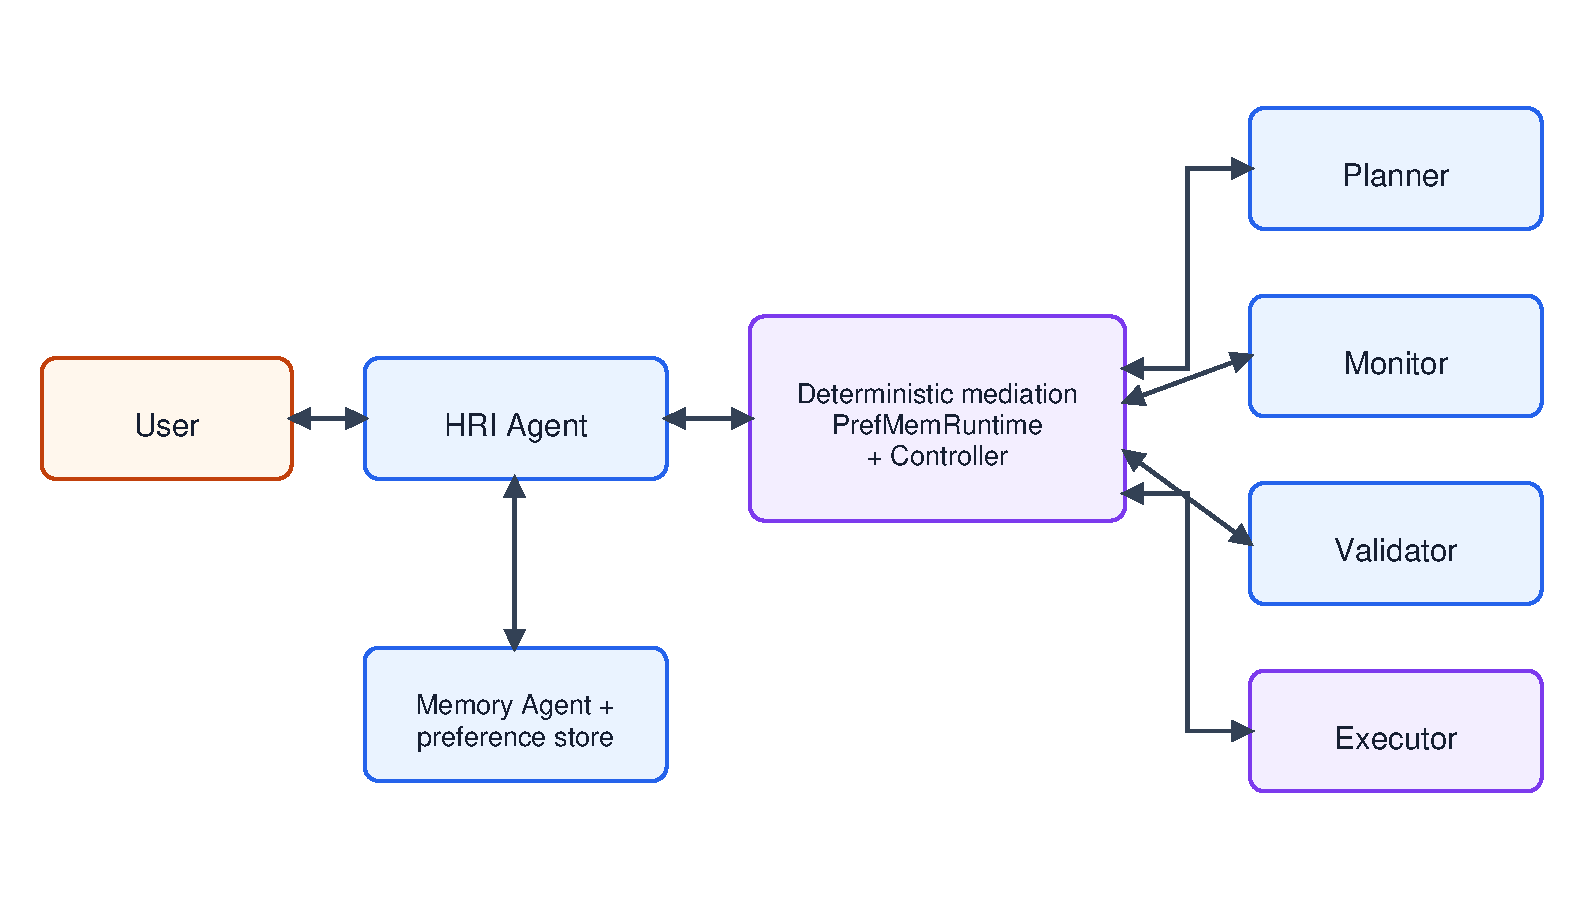
\includegraphics[width=0.92\textwidth]{figures/interaction-protocol.pdf}
    \caption{High-level inter-agent authority graph. Every role-specific path is
    mediated by Runtime or Controller; no unrestricted mutable state is shared
    between agents.}
    \label{fig:interaction-protocol}
\end{figure}

Appendix Table~\ref{tab:interaction-contracts} lists the corresponding typed
artifacts and authority rules.

The complete interaction sequence has three phases. First, HRI and optional
Memory evidence produce a preview, the user confirms its exact identity, and
Validator freezes the checklist. Second, Controller repeatedly requests a fresh
Planner decision, publishes one task, and records stable Monitor evidence.
Third, Planner requests final validation, Validator accumulates checklist
evidence, and host aggregation either completes the goal, returns an incomplete
record to planning, or asks for a new camera view. Attention and emergency
paths can interrupt any active publication without altering the confirmed goal.

\begin{figure}[!htbp]
    \centering
    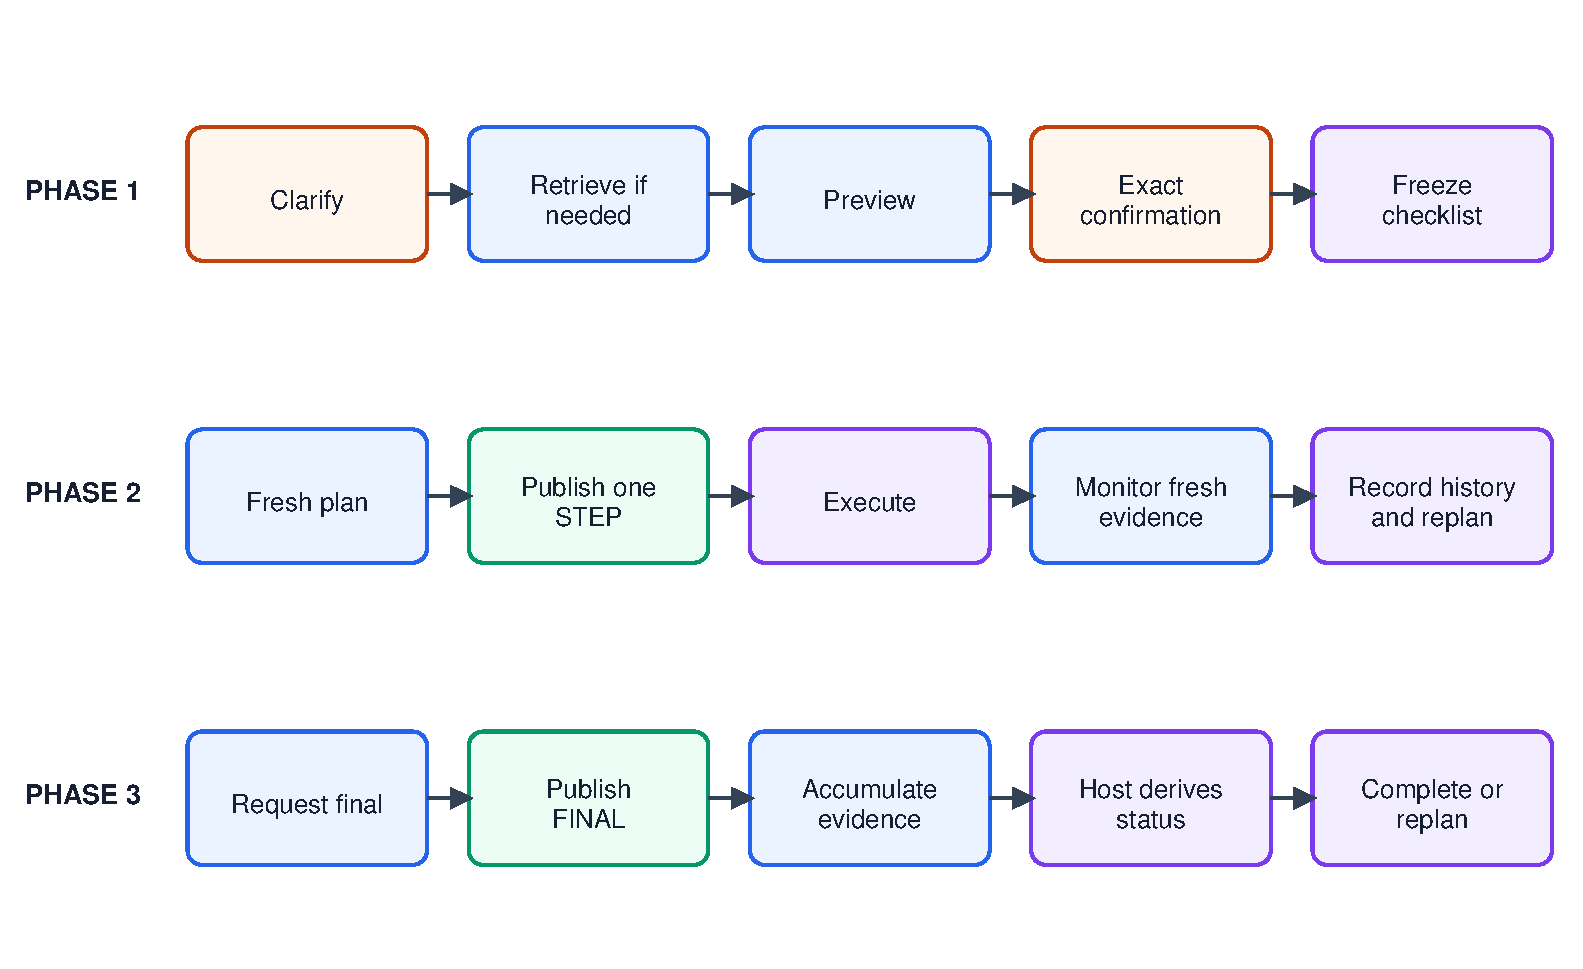
\includegraphics[width=0.90\textwidth]{figures/interaction-sequence.pdf}
    \caption{Expanded three-phase interaction sequence: contract formation,
    receding-horizon execution, and independent final validation. Attention and
    emergency routes may interrupt either active phase.}
    \label{fig:interaction-sequence}
\end{figure}

\subsection{Deployment and Resource Model}
\label{subsec:methodology-deployment}

The five logical agents share one primary reasoning endpoint rather than loading
five model copies. Development model selection favoured a mixture-of-experts
model near 30 billion total parameters and approximately 4 billion active
parameters as a practical balance between semantic capability and inference
speed. PrefMem therefore uses the instruction-tuned Gemma 4 26B A4B model,
whose model card reports approximately 27 billion resident parameters and a
4-billion-active MoE architecture \parencite{gemmateam2026gemma4}. Active
parameters reduce per-token compute, but the full BF16 weights remain resident;
their raw parameter storage is approximately 54 GB before KV cache, vision,
runtime, and allocation overhead.

The primary vLLM endpoint is configured with BF16 precision, batch size one, a
32,768-token maximum sequence, and a GPU-memory-utilisation target of 0.95. On
the 96 GB RTX PRO 6000 Blackwell workstation GPU
\parencite{nvidia2026rtxpro6000}, development runs used approximately 90\% of
device memory. The utilisation target is an allocator configuration rather
than a scientific measurement; the final reproducibility package should retain
the exact launch command and profiler or \texttt{nvidia-smi} evidence. KV-cache
memory grows with sequence length and is a major serving constraint
\parencite{kwon2023pagedattention}, reinforcing the decision to provide each
logical role with targeted context rather than a union of all histories and
tools.

The longer-term design aim is local execution on one edge compute node, but
the current development topology retains separately configurable
EmbeddingGemma and SAM endpoints. Consolidating every service on one GPU is
therefore a target, not a demonstrated property of the evaluated system. The
RTX PRO 6000 is a workstation-class GPU rather than a consumer device. Jetson
AGX Orin offers at most 64 GB in its documented configurations
\parencite{nvidia2026jetsonorin}, while Jetson Thor modules offer larger but
SKU-dependent edge-memory budgets \parencite{nvidia2026jetsonthor}. Full-BF16
Gemma deployment on smaller embedded targets would require quantisation,
offloading, shorter context, or a smaller model.

A future learned VLA will add action-model weights, visual tokens, action cache,
and real-time control constraints. The available context or precision budget
may consequently need to shrink. The narrow \texttt{PublishedTask} interface
and role-specific contexts allow this executor to be integrated without
expanding the HRI, Memory, Monitor, or Validator prompts. The internal model-
selection sweep was an engineering activity rather than a registered
experiment; the thesis should not generalise its choice as a universal optimum
without a matched accuracy, latency, token, and peak-memory comparison.

\subsection{Recovery and Software-Safety Boundary}
\label{subsec:methodology-recovery}

Model, camera, schema, publication, and service errors enter an explicit
attention state with their reason preserved. When a current publication exists,
the operator may resume it with a new attempt identity or request replanning
with guidance. Resumption republishes the same instruction under a new attempt
identity; operator-requested replanning retires the current publication and
records an interruption when applicable. Neither route changes the frozen goal.

The default \texttt{AUTO\_REPLAN} policy applies only to ordinary step
publications. Runtime defers the visual no-progress timeout while the lower-
level executor is still preparing or moving. At timeout, Controller retires the
exact publication, records an \texttt{INTERRUPTED} outcome with typed timeout
context and last accepted evidence, captures a strictly newer frame, and starts
a new planning cycle. Consecutive and per-normalised-instruction timeout guards
bound automatic recovery. Final-validation timeouts, an attention-gate policy,
exhausted guards, or failure while retiring and replanning enter attention;
timeout is never fabricated as Monitor \texttt{FAIL} because lack of progress
is not visual proof of physical failure.

Open-category goals may use a frozen \texttt{DynamicObjectScope} whose
membership remains live. A confirmed new object during motion requests
cancellation and safe hold before replanning. Stack collapse or regression is
handled through ordinary Monitor and Validator evidence rather than privileged
simulator state.

Monitor, Validator, or the operator may also request the shared emergency
latch. This stops further publication in the current process and invokes the
configured stop hook once. The mechanism is a software control boundary, not a
safety-rated emergency system; the current hook does not constitute real-robot
safety certification.

\subsection{Requirement-to-Evidence Traceability}
\label{subsec:methodology-traceability}

Table~\ref{tab:requirement-traceability} maps the design requirements to their
principal implementation and evaluation families. It prevents a learned
component from receiving credit for deterministic host behaviour and prevents
a successful physical state from hiding an upstream semantic error. Exact
results and uncertainty are deferred to the Results chapter.

The complete mapping is provided in Appendix
Table~\ref{tab:requirement-traceability}.


\section{Experiments and Evaluation}
\label{sec:experiments-evaluation}

\subsection{Evaluation Objectives and Claim Boundary}
\label{subsec:evaluation-objectives}

The evaluation asks whether PrefMem's explicit preference, confirmation,
replanning, monitoring, and validation boundaries produce the behaviours for
which they were designed. It does not attempt to estimate a single notion of
``robot intelligence.'' The five research questions from
Section~\ref{subsec:research-problem} are operationalised as distinct outcomes:
autonomous resolution of an omitted field, abstention under missing or
conflicting evidence, explicit-current-over-historical precedence, preference
lifecycle integrity, correct task-level routing, and confirmed physical goal
achievement. Appendix Table~\ref{tab:app-rq-traceability} maps each question to
its primary experiment, comparison, inferential unit, and outcome.

The complete catalogue contains 107 finished experiments: 14 readiness and
calibration studies, 32 isolated component studies, 12 named-interface studies,
seven cumulative workflow studies, nine ablations, 24 original end-to-end
cases, and nine focused thesis experiments. Here, \emph{finished} means that
the registered observations and report exist; it is not a performance label.
The run accounting is provided in Appendix
Table~\ref{tab:app-run-accounting}. Because these layers have different units,
controls, and purposes, they are not pooled into a suite-wide pass rate.

The focused experiments, EXP-01 through EXP-09, provide the principal evidence
for the thesis claims. Readiness, component, interface, workflow-ladder, and
original end-to-end results instead establish measurement validity, expose
integration mechanisms, or motivate the focused contrasts. The evaluation is
development and non-confirmatory unless a particular focused protocol and
freeze file explicitly fixed its cases, conditions, and scoring before
execution. No experiment compares PrefMem with a trained VLA or a monolithic
all-tools agent. The evidence can therefore support boundary-specific claims
about PrefMem in the registered tabletop domain, but not VLA superiority,
general household competence, or universal benefit from multi-agent
decomposition.

\subsection{Experimental Platform and Fixed Configuration}
\label{subsec:evaluation-platform}

Experiments use the fixed \texttt{TB6C-v2} MuJoCo scene: a Franka Emika Panda,
one white board, one cyan board, and red, green, blue, yellow, purple, and orange
cubes. Semantic agents receive the registered third-person \texttt{prefmem}
view, which includes the robot. The execution adapter receives the synchronised
robot-hidden \texttt{sam} RGB-D view. Hidden simulator state is unavailable to
the agents and is used only to verify resets, score placement geometry, and
adjudicate physical outcomes. This creates a separation between ordinary visual
evidence and scoring authority.

The evaluated semantic roles share the primary Gemma 4 reasoning endpoint but
retain the role-specific prompts, schemas, images, and tool surfaces described
in Section~\ref{sec:methodology}. EmbeddingGemma supplies normalised retrieval
vectors; SAM 3.1 supplies source and target masks; calibrated RGB-D produces
world-frame anchors; and the deterministic Panda controller executes supported
pick/place programs. Model version, decoding configuration, prompt and schema
hashes, camera identity, scene/reset identity, and controller configuration are
recorded with each applicable attempt.

Unless an ablation changes a named policy, the full workflow uses two
consistent assessments for stable success or failure, a 30-second ordinary
STEP no-progress timeout, a 20-cycle goal guard, and a two-consecutive-timeout
automatic-replan guard. Executor-active intervals are exempt from the visual
no-progress timeout. Paired conditions share the same language context, scene
state, frame sequence, timing, and host configuration; only the registered
treatment boundary differs.

\subsection{Evaluation Design}
\label{subsec:evaluation-design}

\subsubsection{Evidence Layers}

The suite follows a layered evidence strategy. Readiness and calibration first
test the scene, camera, reset, logging, deterministic safety routes, selector
coverage, anchor geometry, and controller/release bias. Isolated component
experiments replace unrelated learned dependencies with deterministic fixtures,
so that one model-facing contract can be examined without another learned role
hiding its errors. Named-interface studies restore exactly one interaction;
the cumulative ladder then records integration behaviour as requirements are
added. Paired ablations estimate selected boundary effects. Finally, focused
experiments exercise preference decisions, longitudinal state, feedback gates,
registered perturbations, and the complete simulated path. Detailed results for
the supporting layers are in Appendices~\ref{app:supporting-results}
and~\ref{app:focused-results}.

This hierarchy prevents two attribution errors. First, a deterministic timeout
or stale-event guard is not credited to a learned Monitor or Planner. Second, a
correct physical placement cannot hide an incorrect goal contract, wrong target
query, assisted grounding call, or false completion decision. Each layer is
scored only at the responsibility boundary it validly exercises.

\subsubsection{Trial Units and Conditions}

One immutable trial identity contains the case and aim, condition, scene/reset
hash, exact utterance, memory snapshot, model and decoding configuration, prompt
and schema hashes, random seed, source version, and artifact profile. Changing
one member produces a new trial rather than silently modifying an old result.

Original component and interface aims normally use eight semantically distinct
contexts with five fixed variants, producing 40 observations. The variants
change phrasing, object order, irrelevant clauses, seed, or registered camera
perturbation; they are not treated as five independent environments or users.
Original end-to-end cases use five variants per case. EXP-01 through EXP-07 use
paired clustered designs: three surface variants are repeated observations,
while the context, scenario, or lifecycle is the inferential unit. EXP-08 uses
three fresh language/seed pairs in each of six families, and EXP-09 uses three
pairs in each of four contract types. These small final studies are reported
descriptively rather than as population reliability estimates.

\subsubsection{Invalid Runs, Retries, and Provenance}

Every attempt is retained. A valid but unfavourable response is a capability
observation and is never rerun to obtain a preferred answer. An unplanned
infrastructure interruption or invalid fixture may be followed only by an
exact-tuple attempt after repair; the original attempt, invalidity reason,
repair, and retry lineage remain in the audit record. Focused experiments
prohibit capability retries and response reuse. A deliberately injected outage
is a valid stimulus, not an infrastructure-invalid run.

The experiment status is therefore separate from behavioural quality. Reports
preserve direct predicates, formal historical envelopes where present, model
calls, tokens, timing, physical-action counts, and evidence paths. Machine-
readable observations and human-readable reports remain in the versioned
experiment-result directory; representative structured outputs are reproduced
in Appendix~\ref{app:representative-outputs}.

\subsubsection{Strict and Assisted Physical Evidence}

Strict grounding requires every source and target selector in an episode to be
resolved through SAM and RGB-D. When a frozen physical experiment explicitly
permits simulator-oracle continuation after a typed grounding failure, the
strict failure remains recorded and the downstream assisted result is reported
separately. Assistance exposes motion, monitoring, or validation behaviour; it
does not convert the strict observation into a pass. Simulator truth likewise
scores physical state but is never supplied to the semantic agents as task
evidence.

\subsection{Metrics and Statistical Analysis}
\label{subsec:evaluation-statistics}

Primary outcomes are direct binary or count predicates rather than a global
experiment flag. Preference studies distinguish autonomous correct resolution
from correctness after an allowed clarification budget. Conflict studies score
pre-resolution commitment, focused clarification, and post-answer correctness.
Execution-loop studies score the registered host route, endpoint advancement,
discrepancy recovery, false completion, false rejection, and correction
request. Physical studies separately score first-action semantics, action
count, strict grounding, simulator-truth goal state, safety, Validator
finalisation, and the complete registered chain.

For a paired clustered binary outcome, let $Y_{cvk}\in\{0,1\}$ denote the
observation from cluster $c$, surface variant $v$, and condition $k$. The
condition mean within a cluster and the paired risk difference are

\begin{equation}
    \bar{Y}_{ck}
    = \frac{1}{V_c}\sum_{v=1}^{V_c}Y_{cvk},
    \qquad
    \widehat{\Delta}
    = \frac{1}{C}\sum_{c=1}^{C}
      \left(\bar{Y}_{cT}-\bar{Y}_{cC}\right),
    \label{eq:cluster-risk-difference}
\end{equation}

where $T$ and $C$ denote treatment and control. Cluster-bootstrap intervals
resample clusters rather than individual paraphrases. Exact cluster sign-flip
tests are secondary when registered and their assumptions hold. Original
matched ablations retain paired risk differences and exact McNemar tests;
unpaired descriptive rates retain direct counts and Wilson intervals where
available. Latency, model calls, prompt burden, and physical actions are
secondary resource outcomes.

Placement scoring uses the settled hidden object centre. For registered target
$(x^\star,y^\star)$, radial error is

\begin{equation}
    e_r = \sqrt{(x_{\mathrm{settled}}-x^\star)^2
                +(y_{\mathrm{settled}}-y^\star)^2}.
    \label{eq:placement-radial-error}
\end{equation}

Signed axis errors are retained because a small radial value can hide a
repeatable directional bias. EXP-08 and EXP-09 intervals are descriptive due
to their three observations per family or contract type. No multiplicity-
adjusted suite-wide hypothesis is constructed, and no denominator combines
readiness rows, dialogue observations, retrieval-grid rows, and physical
episodes.

\subsection{Readiness and Supporting Diagnostic Results}
\label{subsec:evaluation-supporting-results}

\subsubsection{Scene, Camera, Reset, and Safety Readiness}

The readiness layer established that the frozen fixture and evidence pipeline
were usable for development experiments. Scene resets reproduced the registered
state; all objects and analytical waypoints were visible or reachable in the
specified distribution; camera projection/deprojection error was negligible;
the reset verifier rejected a displaced-object negative control; and the eight
replanning plus twelve safety replays followed their registered deterministic
routes. These results validate measurement and host ordering, not learned
semantic competence or real-robot safety. Complete counts and qualifications
are reported in Appendix Table~\ref{tab:app-readiness-calibration}.

\subsubsection{Grounding and Placement Calibration}

Calibration separated three mechanisms. Projection and oracle-mask anchor
estimation were sub-millimetre at their principal quantiles. SAM masks were
high quality conditional on detection, but detection covered only 355 of 520
selector-position observations. Oracle-coordinate and full-path placement both
retained an approximately $+4$ mm signed $x$-shift, localising much of the
bias to grasp, controller, release, or contact dynamics rather than camera
geometry. The stage-specific results are in Appendix
Table~\ref{tab:app-readiness-calibration}; consequently, no global perception
correction is claimed.

\subsubsection{Component and Interface Diagnostics}

The broad component studies show why later focused endpoints were required.
HRI was strongest on typed runtime state and preference policy but weaker on
unresolved material ambiguity. Planner used trusted history and completion
routes reliably but showed lower spatial-grounding and capability-fence
accuracy. Deterministic Memory candidate construction was correct in 40/40
rows, whereas four original semantic Memory aims stopped before inference due
to a checkpointer/thread configuration defect. Monitor and Validator preserved
several host invariants but remained visually overconfident or insufficiently
uncertain in difficult states. Compiler permissiveness, SAM coverage, and IK
exceptions formed separate executor limitations.

The cumulative ladder is retained as an integration diagnostic, not a causal
component ranking, because each level adds both a component and additional
required predicates. The original Memory level in particular exposed a harmful
integration seam rather than proving that preference memory is intrinsically
harmful. Appendix Table~\ref{tab:app-component-diagnostics} reports the direct
component results and their interpretation boundaries.

\subsection{Preference-Aware Intent Evaluation}
\label{subsec:evaluation-preference}

\subsubsection{Applicable Scoped Memory}

EXP-01 compares the same under-specified utterance with applicable scoped
Memory, empty Memory, and an exact-instruction ceiling. Scoped Memory produced
autonomous correct resolution in 36/36 observations versus 0/36 with empty
Memory, a paired difference of $+1.00$ with all twelve cluster differences
positive. Both conditions nevertheless reached 36/36 correct goals within the
two-turn budget. The contribution is therefore a one-turn reduction in
interaction cost, not an increase in attainable correctness. Only 9/36
populated observations returned a perfectly scoped candidate set, so the
effect belongs to the combined HRI--Memory decision boundary rather than raw
retrieval precision. Condition tables and plots are in Appendix
Table~\ref{tab:app-intent-results} and
Figure~\ref{fig:app-intent-results}.

\subsubsection{Conflict-Aware Abstention}

EXP-02 tests whether caution is selective rather than universal. Two equally
scoped conflicting records caused no pre-resolution goal in 36/36 observations,
focused clarification in 36/36, and the correct post-answer goal in 36/36. A
unique applicable record remained autonomous in 35/36. The system therefore
distinguished unique evidence from conflict instead of simply selecting the
top retrieved item. However, wrong-task candidates were excluded in only 21/36
unique-Memory observations; downstream reasoning compensated for noisy
retrieval rather than eliminating it. Detailed condition and resource outputs
are in Appendix Table~\ref{tab:app-intent-results}.

\subsubsection{Explicit Current-Instruction Override}

EXP-03 and EXP-04 test field-level composition: Memory may supply an omitted
usual cube, but the board explicitly named in the current instruction must not
be replaced by a historical board. The original EXP-03 measurement was
sensitive to how yes/no clarification was observed and is preserved unchanged.
The held-out EXP-04 replication used new users, tasks, wording, and cube
assignments with a corrected clarification observer. In the opposing-Memory
condition, the explicit board was preserved in 35/36, the correct goal was
reached within budget in 35/36, and the historical board was selected in 0/36.
The result supports current-over-historical precedence at the tested fields,
while the remaining wrong-task retrievals constrain any claim about retrieval
scope. Appendix Table~\ref{tab:app-intent-results} retains both the original and
replication results.

\subsubsection{Longitudinal Preference Lifecycle}

EXP-05 carries eight independent stores through 30 ordered interactions without
an in-lifecycle reset. Initial creation, immediate direct recall, and initial
HRI use were 8/8. Explicit update and updated-value recall were 7/8, while
updated HRI use was 5/8. After fourteen semantically related distractor
mutations, delayed direct recall was 2/8, delayed HRI use was 3/8, and final
direct recall remained 2/8. Store serialization stayed consistent in 240/240
interactions and the old value remained absent after update, but free-text
mutation arbitration sometimes reused or replaced the wrong semantic identity.

This is a decisive negative result for unrestricted long-term-memory claims.
The prototype supports a clean short lifecycle but does not robustly preserve a
focal preference under repeated related mutations. The full trajectory is in
Appendix Table~\ref{tab:app-memory-lifecycle} and
Figure~\ref{fig:app-memory-lifecycle}; it motivates immutable structured user,
task, preference-dimension, and provenance keys.

\subsection{Execution-Loop Evaluation}
\label{subsec:evaluation-execution-loop}

\subsubsection{Fresh Replanning}

The stable-failure ablation recovered 40/40 deterministic traces with fresh
replanning and 0/40 with a frozen action queue. The timeout-policy ablation
recovered 40/40 under both automatic and attention-gated policies, but automatic
replanning required zero operator interventions rather than 45 and introduced
no registered stale action or guard breach. These experiments justify retiring
stale task queues and show an interaction-cost benefit at the deterministic
host-policy boundary. Because the Planner outputs were fixtures, they do not
establish learned Planner quality. Appendix Table~\ref{tab:app-replanning}
contains the paired results.

\subsubsection{Monitor Ablation}

EXP-06 holds the host timing, publications, frames, and scenario clusters fixed
while replacing production Monitor with a control that never claims visual
advancement. Production Monitor produced the expected host route in 22/36
observations versus 12/36 for the control, a $+27.8$ percentage-point paired
change with a cluster-bootstrap 95\% interval from $+8.3$ to $+50.0$
points. It advanced 7/9 stable endpoints and registered 3/3 visible-progress
cases, but recovered only 3/15 visual discrepancies; seven of 78 invocation
attempts were schema-invalid. Host holds and timeouts were equal in both
conditions and are not credited to the learned Monitor. Appendix
Table~\ref{tab:app-feedback-results} and
Figure~\ref{fig:app-feedback-results} separate these functions.

\subsubsection{Validator Ablation}

EXP-07 compares production Validator with stopping after actions and assuming
success. On 21 visibly incomplete observations, production Validator produced
zero false completions and requested correction in all 21; the control falsely
completed all 21. On genuinely complete states, production finalised 14/15
versus 15/15 for the control. Independent validation therefore provides a large
false-completion benefit with a measurable false-rejection cost. The result
justifies a separate completion gate but not unquestioned Validator authority;
its detailed routes and criterion accuracy appear in Appendix
Table~\ref{tab:app-feedback-results} and
Figure~\ref{fig:app-feedback-results}.

\subsection{Robustness and End-to-End Evaluation}
\label{subsec:evaluation-end-to-end}

\subsubsection{Focused Competency Envelope}

EXP-08 uses three fresh language/seed pairs in each of six families: slip,
timeout, occlusion, planned outage, scoped preference, and explicit override.
The complete registered family-specific event occurred in 15/18 episodes and
the registered safety condition in 18/18. Occlusion, outage containment, and
scoped preference occurred in 3/3 each; slip and timeout recovery occurred in
2/3 each. Fourteen episodes completed strictly, two used separately recorded
oracle assistance, and two stopped safely at selector/grounding. The two
unreached recovery stimuli failed on unsupported aliases before the intended
perturbation, localising the mechanism to language-to-selector normalisation.
Family-level outcomes are reported in Appendix
Table~\ref{tab:app-competency-envelope}. With only three episodes per family,
this is a demonstrated envelope rather than a broad robustness estimate.

\subsubsection{Simulated Intent-to-Outcome Evaluation}

EXP-09 follows twelve fresh episodes across omitted-board, omitted-cube,
explicit-override, and user-scoped contracts. Expected Memory records, correct
goal contracts, confirmation, and correct first compiled actions occurred in
12/12, with no wrong target-board query. All twelve reached the registered
simulator-truth physical arrangement safely. Eleven remained strict through
all SAM grounding calls, nine were finalised by Validator, and eight satisfied
the exact one-action all-strict chain. Contract-specific results and the stage
funnel are in Appendix Table~\ref{tab:app-end-to-end} and
Figure~\ref{fig:app-end-to-end-funnel}.

The three omitted-cube episodes illustrate why stage-level scoring is necessary.
All placed blue at the cyan-board centre within the physical tolerance, but
Monitor or Validator rejected the low-contrast state and caused repeated
actions or attention. Thus intent and physical goal achievement were 12/12 even
though terminal visual closure was 9/12. EXP-09 begins from frozen exact
preference fixtures and therefore tests application of retrieved evidence, not
production retrieval accuracy. Representative successful and false-negative
outputs appear in Appendix~\ref{app:representative-outputs}.

\subsection{Threats to Validity}
\label{subsec:evaluation-validity}

\paragraph{Internal validity.}
The original suite is development/non-confirmatory evidence, and some source
state evolved after early source-lock hashes. Several original semantic Memory
aims were blocked before inference by a configuration defect, and several
controlled recovery events fired at an illegal host phase or were not reached.
These observations are retained as integration diagnostics rather than
relabelled learned failures. EXP-03's clarification-observer sensitivity is
reported beside, not replaced by, the held-out EXP-04 replication.

\paragraph{Construct validity.}
Some original rubrics were overly lexical; for example, semantically adequate
scene descriptions could fail a required word. Sensitivity audits are reported
without overwriting frozen scores. Hidden simulator pose is a precise physical
authority but does not reproduce real sensor uncertainty. Expected host routes
are responsibility-specific proxies and must not be interpreted as general
task intelligence. Strict and assisted grounding are kept separate to prevent
oracle continuation from inflating learned perception evidence.

\paragraph{External validity.}
Physical results use one MuJoCo tabletop scene, one embodiment, two boards, six
cubes, and one fixed camera family. EXP-08 and EXP-09 contain only three fresh
episodes per family or contract type. The work therefore does not establish
real-robot safety, open-world language understanding, long-horizon household
generalisation, or robust preference retention over hundreds of interactions.

\paragraph{Statistical validity.}
Surface variants are correlated repetitions, so focused uncertainty resamples
clusters. Twelve clusters can identify large consistent changes but provide
limited precision for heterogeneous effects; three-case families are
descriptive. Multiple secondary predicates are mechanism analyses rather than
independent confirmatory hypotheses, and no favourable stopping rule or
capability rerun was used.

\paragraph{Comparative validity.}
No trained VLA or single-agent all-tools baseline was evaluated. The evidence
supports the selected architecture through boundary-specific effects,
containment, and failure localisation, not through an empirical claim that
multi-agent graph/loop engineering always outperforms a monolithic system.

\subsection{Evaluation Summary}
\label{subsec:evaluation-summary}

The evaluation answers the research questions with a mixed but coherent
result. Applicable preference evidence reduced dialogue by one turn without
changing attainable correctness. Conflicting evidence caused abstention, and a
held-out replication preserved explicit current fields over history. The
longitudinal study rejected a strong robust-memory claim by exposing free-text
identity loss. Fresh replanning, Monitor, and Validator produced distinct
benefits at their own boundaries, while Monitor discrepancy recovery and
Validator false rejection remained important weaknesses. Finally, twelve
focused simulated episodes preserved intent through physical outcome, but
visual finalisation reduced the exact strict-chain count. PrefMem's supported
contribution is consequently an inspectable preference-and-evidence control
architecture with measurable boundary effects and localised failure mechanisms,
not a universal improvement score.


\section{Discussion}
\label{sec:discussion}

\subsection{Interpretation of the Main Findings}
\label{subsec:discussion-findings}

PrefMem addresses a task-level problem that is not solved by predicting a robot
action alone: maintaining a trustworthy agreement about what the robot should
do, why a historical preference is applicable, when the robot must ask, and
what evidence permits completion. The evaluation supports this framing while
showing that explicit boundaries do not make every learned decision reliable.
Detailed measurements are reported in Section~\ref{sec:experiments-evaluation}
and Appendices~\ref{app:supporting-results}--\ref{app:representative-outputs};
this chapter interprets their combined implications.

The strongest positive result is selective use of preference evidence. One
applicable record removed a clarification turn without changing final
correctness; equal conflict caused abstention; and a held-out replication
preserved a current explicit board against opposing history. PrefMem therefore
implements more than generic personalisation: history may fill an omitted field
only when its scope and provenance justify doing so. This complements systems
that infer household preferences from examples
\parencite{wu2023tidybot,wang2024apricot} by emphasising authority, confirmation,
conflict, and revocability before action.

Fresh replanning, Monitor, and Validator also produced distinct effects. Fresh
replanning retired a failed queue; Monitor supplied endpoint and progress
evidence; and Validator prevented every registered false completion in visibly
incomplete scenes. These roles operate at different temporal scales and prevent
an action attempt, a local success, or a Planner prediction from becoming
whole-goal evidence merely because it occurs late in a sequence.

The evidence does not support a claim that every additional agent improves the
complete stack. The cumulative ladder was not monotonic, the old Memory
integration was harmful on its development endpoint, Monitor recovered only a
minority of visual discrepancies, and Validator sometimes rejected correct
states. Most importantly, delayed preference recall survived mutation pressure
in only two of eight stores. The project has implemented and evaluated the
preference lifecycle, but has not solved robust long-term personal memory.

The focused end-to-end study illustrates the value of staged evaluation. All
twelve episodes formed the intended contract and reached the registered
physical arrangement, whereas nine received Validator completion and eight
satisfied the exact one-action strict chain. A global score would hide whether
a failure arose from intent, grounding, action efficiency, physical outcome, or
visual closure. PrefMem's central systems contribution is that these stages are
represented by named contracts, publications, evidence, and authorities.

\subsection{Project Achievements}
\label{subsec:discussion-achievements}

\subsubsection{Preference-Aware Task Contracts}

The first achievement is a conservative interaction policy. PrefMem retrieves
before deciding, fills only a missing field from one applicable record, asks
under conflict, preserves current explicit values, and separates physical goal
confirmation from consent to change future memory. Embedding similarity is
candidate generation rather than authority; HRI still evaluates user, task,
field, and wording. This is an appropriate default for manipulation because a
wrong physical commitment is costlier than one focused question.

The tested ambiguities concern known cube, board, and order fields rather than
open-world intention understanding. Nevertheless, they represent a practical
household interaction pattern: users omit habitual details. The project shows
that these omissions can be governed through explicit scope, provenance, and
abstention instead of an undocumented prompt convention.

\subsubsection{Inspectable Graph and Loop Engineering}

The second achievement is an explicit control graph. HRI, Memory, Planner,
Monitor, Validator, Runtime, Controller, and the executor exchange typed goal
proposals, contracts, publications, assessments, history records, and
notifications rather than sharing an unrestricted conversation. Models propose
semantic content; deterministic host code confirms goals, publishes actions,
owns history, applies guards, and establishes completion.

Loop engineering supplies temporal discipline. One task is published, only
post-publication evidence is accepted, stable outcomes retire the old identity,
and the next cycle uses a fresh frame. Final validation is a separate bounded
loop over a frozen checklist. This extends feedback-based embodied reasoning
\parencite{ahn2022saycan,huang2022innermonologue,yao2023react} with explicit
preference provenance, publication identity, confirmation, and terminal
evidence.

One all-tools agent could reproduce much nominal behaviour. Role separation is
useful because each role needs different context, temporal scope, and authority:
Memory sees preference tools, Planner sees the frozen goal, Monitor sees one
publication, Validator sees the whole checklist, and only HRI addresses the
user. This improves failure localisation and supports shorter role-specific
contexts on edge hardware. It is an implemented authority architecture, not yet
an empirical proof of superiority over a matched monolithic agent.

\subsubsection{Independent Evidence and Completion}

The third achievement is separation of progress from completion. Monitor is
step-bound, Validator is goal-bound, and Controller aggregates their evidence.
Executor return is not visual success; finishing an action list is not proof of
the goal; and Planner cannot certify its own plan. Validator's prevention of all
registered incomplete-state completions directly supports this boundary, while
its false rejection quantifies the cost of imperfect evidence.

Monitor's contribution is smaller but distinct: it advanced endpoints and
registered progress that the no-visual control could not. Deterministic holds
and timeouts were unchanged, correctly locating those behaviours in host policy
rather than learned vision. The architecture therefore permits both benefit and
failure cost to be assigned to the responsible layer.

\subsubsection{End-to-End Feasibility and Research Deliverables}

The fourth achievement is a functioning preference-to-physical-state path. In
the focused MuJoCo study, the system applied the expected record, confirmed the
goal, issued the correct first compiler request, and reached the physical outcome
in all twelve episodes; eleven remained strict through SAM grounding. The
executor is supporting infrastructure, not a new VLA. Its narrow boundary makes
PrefMem complementary to semantic and hierarchical VLA research
\parencite{ni2026semanticvla,shi2025hirobot,yang2025agenticrobot,li2026roboclaw}.

The project also delivers typed control software, scoped Memory, human and
MuJoCo adapters, calibration, bounded recovery, evidence recording, component
fixtures, focused protocols, and a 107-experiment catalogue. Strict and assisted
runs remain separate, invalid attempts retain lineage, and capability failures
are not rerun for replacement. Retaining positive, null, and negative evidence
is itself important for an auditable systems contribution.

\subsection{Shortcomings and Failure Analysis}
\label{subsec:discussion-shortcomings}

\subsubsection{Memory Identity and Scope}

The most serious shortcoming is free-text memory identity. Retrieval often
returned useful records alongside wrong-task candidates, and HRI compensation
does not make that retrieval precise. Mutation arbitration sometimes treated a
related new preference as an update across task scope or user ownership. The
store stayed structurally valid while the intended semantic identity was lost.
Similarity is suitable for search but not as a primary key for ownership,
dimension, supersession, or revocation; increasing store or context size would
not address this mechanism.

\subsubsection{Semantic and Interface Brittleness}

HRI sometimes previewed unresolved requests; Planner was weaker on spatial
relations and capability fencing; the compiler accepted too many unsupported
instructions; and healthy Monitor calls sometimes violated the schema. Typed
parsing contains malformed responses but cannot correct a schema-valid semantic
error. Conversely, brittle lexical evaluation can reject a semantically useful
answer. The present system still relies heavily on prompting rather than a
canonical task language shared across roles.

\subsubsection{Visual Feedback and Correlated Error}

Monitor recovered only 3/15 registered visual discrepancies. Validator rejected
some correct states, including all three low-contrast blue-on-cyan finalisations
in EXP-09, causing redundant action or attention despite correct physical
placement. Role separation provides procedural independence, not statistical
independence: the roles share one Gemma endpoint and similar views, so correlated
perceptual error remains possible.

\subsubsection{Execution and Integration Boundaries}

The surrogate has vocabulary, detection, and control limits. Reasonable aliases
may fall outside the selector vocabulary; SAM is accurate when detected but has
coverage gaps; isolated actions can encounter IK exceptions; and successful
placements retain an approximately $+4$ mm signed $x$-bias. Several original
Memory and recovery tests also measured configuration or event-injection seams
rather than the intended learned capability. Modularity improves observability
but creates interfaces that must be versioned and tested; the present design
makes these failures inspectable without yet making every seam robust.

\subsection{Limitations}
\label{subsec:discussion-limitations}

\paragraph{Scope and evidence.}
Physical evidence uses one MuJoCo tabletop scene, one Panda, two boards, six
cubes, and one camera family; it does not establish real-robot transfer or
safety. Most evidence is development and non-confirmatory, with clustered
paraphrases and small focused families. The results locate large effects and
mechanisms rather than broad reliability.

\paragraph{Baselines and users.}
There is no trained VLA, matched monolithic agent, or model-size comparison.
Deterministic replanning isolates host policy, and frozen EXP-08/09 preference
fixtures do not estimate production retrieval. Scripted turns also do not
measure satisfaction, trust, clarification tolerance, or consent comprehension.

\paragraph{Model and executor validity.}
All semantic roles share one Gemma-family endpoint, and the workstation result
does not prove that a VLA-integrated stack fits one edge GPU. The compiler,
SAM, RGB-D, and deterministic IK approximate a VLA interface but not continuous
learned-action uncertainty, policy latency, or embodiment-conditioned recovery.

\subsection{Future Work}
\label{subsec:discussion-future-work}

Future work should proceed in the following order:

\begin{enumerate}
    \setlength{\itemsep}{2pt}
    \setlength{\parsep}{0pt}
    \item \textbf{Structure preference identity.} Give each record immutable
    user, task, dimension, object, provenance, and supersession keys. Host code
    should classify create, update, revoke, or conflict before a model proposes
    text, and writes should be transactional. A held-out EXP-05 replication
    should measure focal survival, scope violations, update identity, and
    revocation over longer histories while retaining the current 2/8 baseline.

    \item \textbf{Canonicalise the task/execution language.} Map aliases,
    objects, target regions, relations, tolerances, and visibility requirements
    into a versioned ontology before compilation. An allowlist grammar should
    reject unsupported actions before motion and be tested on held-out aliases,
    not tuned against EXP-08 failures.

    \item \textbf{Calibrate Monitor and Validator.} Combine VLM semantics with
    segmentation, depth geometry, and multiple views. Treat unknown as a
    calibrated outcome. A held-out low-contrast set should measure false
    completion and false rejection together; constrained decoding and an
    independent model or sensor path could reduce malformed and correlated
    errors.

    \item \textbf{Test architecture and VLA integration.} Compare the graph
    with a matched all-tools agent under the same model, prompt content, calls,
    tokens, and GPU budget; measure accuracy, authority violations, latency,
    VRAM, and failure localisation. Then substitute a frozen VLA through
    PublishedTask without granting preference, goal-revision, or completion
    authority.

    \item \textbf{Expand physical, human, and confirmatory evaluation.} Re-run
    focused cases on a supervised robot with independent pose scoring, and use a
    separate approved study for clarification burden, trust, and consent.
    Report edge-resource use and freeze broader users, tasks, layouts, histories,
    endpoints, and scorers before inspection, while retaining stage-specific
    outcomes.
\end{enumerate}

\subsection{Concluding Perspective}
\label{subsec:discussion-conclusion}

PrefMem makes preference, confirmation, planning, monitoring, and validation
explicit contracts around an executor. Evidence supports selective memory use,
replanning, completion gating, and simulated feasibility while exposing memory
and visual limits. The contribution is an inspectable authority-and-evidence
architecture.


\clearpage
\appendix
\numberwithin{figure}{section}
\numberwithin{table}{section}

\section{Experimental Design and Run Accounting}
Core results are summarised below. Complete experiment reports and artifacts
are available in:
\url{https://liveuclac-my.sharepoint.com/:u:/g/personal/ucabibp_ucl_ac_uk/IQCUJvx2H20nSIxwF1vrFhgmAYJn0NPS3Deujkp-VIlDPq8?e=Lcfqzm}.
\label{app:experiment-design}

\subsection{Run Accounting}

{\small
\renewcommand{\arraystretch}{1.12}
\begin{longtable}{@{}P{2.45cm}P{3.95cm}P{1.55cm}P{1.55cm}P{4.70cm}@{}}
    \caption{Experiment-suite run accounting. A finished experiment has a
    complete registered observation set and report; the term is not a quality
    verdict.}
    \label{tab:app-run-accounting} \\
    \toprule
    \textbf{Layer} & \textbf{Purpose} & \textbf{Count} &
    \textbf{Finished} & \textbf{Interpretation} \\
    \midrule
    \endfirsthead
    \caption[]{Experiment-suite run accounting (continued).} \\
    \toprule
    \textbf{Layer} & \textbf{Purpose} & \textbf{Count} &
    \textbf{Finished} & \textbf{Interpretation} \\
    \midrule
    \endhead
    \bottomrule
    \endlastfoot
    Readiness and calibration & Validate fixture, evidence, geometry, and
    execution measurements & 14 & 14 & Measurement and mechanism evidence; not
    semantic performance \\
    Isolated components & Exercise one role contract with fixture replacements
    & 32 & 32 & Component diagnostics with responsibility-specific predicates \\
    Named interfaces & Restore exactly one agent/host interaction & 12 & 12 &
    Propagation and containment evidence \\
    Workflow ladder & Add cumulative requirements across ambiguity contexts & 7
    & 7 & Integration diagnostic; adjacent rates are not pure component effects \\
    Ablations & Compare selected paired boundaries and host policies & 9 & 9 &
    Direct effects only at the frozen replacement boundary \\
    Original end to end & Nominal, ambiguity, and recovery development cases &
    24 & 24 & Broad development evidence with mixed upstream/downstream failure \\
    Focused studies & Paired claim studies, robustness envelope, and
    fresh simulated chain & 9 & 9 & Principal thesis evidence \\
    \textbf{Total} & & \textbf{107} & \textbf{107} & No suite-wide success
    percentage is defined \\
\end{longtable}
}

\subsection{Research-Question Traceability}

{\small
\renewcommand{\arraystretch}{1.12}
\begin{longtable}{@{}P{0.75cm}P{3.80cm}P{3.00cm}P{2.30cm}P{4.30cm}@{}}
    \caption{Research questions, primary evidence, and outcomes.}
    \label{tab:app-rq-traceability} \\
    \toprule
    \textbf{RQ} & \textbf{Operational question} & \textbf{Primary evidence} &
    \textbf{Inferential unit} & \textbf{Primary outcomes} \\
    \midrule
    \endfirsthead
    \caption[]{Research-question traceability (continued).} \\
    \toprule
    \textbf{RQ} & \textbf{Operational question} & \textbf{Primary evidence} &
    \textbf{Inferential unit} & \textbf{Primary outcomes} \\
    \midrule
    \endhead
    \bottomrule
    \endlastfoot
    1 & Does one applicable scoped preference resolve an omitted field without
    dialogue? & EXP-01 & 12 context clusters & Autonomous correct goal,
    within-budget correctness, clarification turns, scope, and safety \\
    2 & Does the system abstain under conflict and preserve current explicit
    fields? & EXP-02, EXP-03, EXP-04 & 12 clusters per study & Pre-resolution
    commitment, clarification, explicit field, historical selection, and
    final goal \\
    3 & Does preference state survive create, update, delay, distraction, and
    revocation? & EXP-05 & Eight independent lifecycles & Direct recall, HRI
    use, identity, scope, retention, revocation, and store consistency \\
    4 & Do fresh replanning, Monitor, and Validator improve their registered
    routes? & AB-RPL-F/T, EXP-06, EXP-07 & 40 paired traces or 12 scenario
    clusters & Recovery, interventions, expected route, false completion,
    correction, and false rejection \\
    5 & Can a confirmed contract reach a safe simulated physical goal? & EXP-08
    and EXP-09 & Six families or four contract types & Registered perturbation
    route, strict/assisted grounding, physical state, safety, validation, and
    exact chain \\
\end{longtable}
}


\clearpage
\section{Supporting Readiness, Calibration, and Diagnostic Results}
\label{app:supporting-results}

\subsection{Readiness and Placement Calibration}

{\footnotesize
\renewcommand{\arraystretch}{1.1}
\begin{longtable}{@{}P{2.25cm}P{1.40cm}P{6.05cm}P{4.95cm}@{}}
    \caption{Readiness and calibration results.}
    \label{tab:app-readiness-calibration} \\
    \toprule
    \textbf{Study} & \textbf{Rows} & \textbf{Direct result} &
    \textbf{Interpretation boundary} \\
    \midrule
    \endfirsthead
    \caption[]{Readiness and calibration results (continued).} \\
    \toprule
    \textbf{Study} & \textbf{Rows} & \textbf{Direct result} &
    \textbf{Interpretation boundary} \\
    \midrule
    \endhead
    \bottomrule
    \endlastfoot
    PF-ASSET & -- & Canonical, relocated, and archived scene dependencies and
    hashes were valid. & Reproducible loading only. \\
    PF-SCENE & 20 & All eight objects were visible; all 28 object pairs remained
    separated; 32 analytical waypoints were reachable. & Fixture distribution,
    not general scene coverage. \\
    PF-CAMERA & 20 pairs & Approved calibration and aligned depth were retained;
    maximum round-trip error was approximately $1.14\times10^{-13}$ px. &
    Camera geometry is not a plausible source of millimetre-scale bias here. \\
    PF-RESET & 20 & Canonical resets reproduced; a displaced-cube negative
    control was rejected before restoration. & Reset-verifier evidence only. \\
    PF-MOTION & 32 & All analytical approach/contact waypoints satisfied IK and
    workspace fences without actuation. & Does not test grasp or release. \\
    PF-SELECTOR & 160 & Intended selectors were detected in 20/20 registered
    perturbations per selector; median radial anchor errors were below 5 mm. &
    Narrower and easier than the CAL-X-03 grid. \\
    PF-REPLAN & 8 traces & Every deterministic replay followed its expected
    fresh-request, retirement, reset, or incompleteness route. & No learned
    Planner calls. \\
    PF-SAFETY & 12 traces & Stale events, errors, guards, attention, and emergency
    latching were contained as registered. & Software invariants, not safety
    certification. \\
    PF-LOG & 3 attempts & Final retained attempt produced a complete artifact
    bundle and a 3.18 mm oracle-coordinate placement. & Artifact-pipeline
    demonstration, not a success rate. \\
    CAL-X-01 & 375 & Median signed error was $+0.015$ mm $x$, $+0.055$ mm
    $y$; p95 absolute axis error was approximately 0.689 mm. & Projection is
    not the dominant (+x) mechanism. \\
    CAL-X-02 & 520 & Oracle-mask anchors were complete; p95 absolute error was
    0.137 mm (x) and 0.662 mm (y). & Accuracy conditional on the correct
    mask. \\
    CAL-X-03 & 520 & SAM detected 355/520; 165 were usable zero-detection
    responses. Conditional mask IoU had minimum 0.952 and median 0.997. & Main
    limitation is selector-position coverage, not successful-mask accuracy. \\
    CAL-X-04 & 300 & All oracle-coordinate placements completed; median error was
    $+3.938$ mm $x$, $-0.012$ mm $y$; p95 radial error 4.180 mm. &
    Localises the repeatable shift to controller/release dynamics. \\
    CAL-X-05 & 300 & Full-path placements completed; median error was $+3.996$
    mm $x$, $-0.700$ mm $y$; p95 radial error 4.594 mm. & Sequential
    development run; does not erase CAL-X-03 coverage gaps. \\
\end{longtable}
}

\subsection{Component Diagnostics}

{\footnotesize
\renewcommand{\arraystretch}{1.1}
\begin{longtable}{@{}P{2.05cm}P{6.00cm}P{3.15cm}P{3.45cm}@{}}
    \caption{Selected component and integration diagnostics.}
    \label{tab:app-component-diagnostics} \\
    \toprule
    \textbf{Boundary} & \textbf{Direct observations} & \textbf{Strength} &
    \textbf{Important limitation} \\
    \midrule
    \endfirsthead
    \caption[]{Selected component and integration diagnostics (continued).} \\
    \toprule
    \textbf{Boundary} & \textbf{Direct observations} & \textbf{Strength} &
    \textbf{Important limitation} \\
    \midrule
    \endhead
    \bottomrule
    \endlastfoot
    HRI & State reporting 39/40; preference policy 33/40; exact tool route 32/40;
    registered broad ambiguity behaviour 21/40. & Typed state and authority
    interfaces. & Material ambiguity sometimes advanced prematurely; lexical
    rubrics affected some scores. \\
    Planner & Next task 37/40; fresh-frame use 37/40; history and completion
    routing 40/40; grounding 22/40; capability fence 32/40. & Fresh explicit
    state and trusted history. & Spatial relation precision and unsupported-
    request fencing. \\
    Memory & Candidate construction 40/40 and empty/undersized-store handling
    40/40. Four original semantic aims stopped before inference. & Deterministic
    capped retrieval layer. & Context disabled to prevent referring to previous decisions. \\
    Monitor & Criteria 35/40; state 25/40; stability 30/40; progress timing 40/40;
    error routing 35/40. & Host timing and progress policy. & Wrong-object, slip,
    and unexpected states often remained ongoing. \\
    Validator & Checklist 35/40 lexically and 40/40 in semantic audit; final
    state 28/40; evidence handling 25/40; reset isolation 40/40. & Checklist
    coverage and lifecycle isolation. & Unsupported certainty and occasional
    false completion/rejection. \\
    Execution surrogate & Supported compiler calls 20/20, unsupported rejection
    5/20; SAM and anchor rows 28/40; oracle-coordinate motion 35/40. & Supports
    a real simulated state change. & Compiler permissiveness, detection coverage,
    and IK are separate limitations. \\
\end{longtable}
}

\subsection{Fresh-Replanning Ablations}

{\small
\renewcommand{\arraystretch}{1.12}
\begin{longtable}{@{}P{2.15cm}P{4.10cm}P{4.10cm}P{4.30cm}@{}}
    \caption{Deterministic host-policy replanning ablations.}
    \label{tab:app-replanning} \\
    \toprule
    \textbf{Study} & \textbf{Treatment} & \textbf{Control} &
    \textbf{Effect and boundary} \\
    \midrule
    \endfirsthead
    \caption[]{Replanning ablations (continued).} \\
    \toprule
    \textbf{Study} & \textbf{Treatment} & \textbf{Control} &
    \textbf{Effect and boundary} \\
    \midrule
    \endhead
    \bottomrule
    \endlastfoot
    AB-RPL-F & Fresh replanning recovered 40/40 stable-failure traces. & Frozen
    queue recovered 0/40. & Planner outputs were deterministic fixtures. \\
    AB-RPL-T & Automatic timeout replanning recovered 40/40 with zero operator
    interventions. & Recovered 40/40 with 45 operator
    interventions. & Same recovery and safety; interaction-cost improvement at
    the host-policy boundary. \\
\end{longtable}
}


\clearpage
\section{Focused Experiment Results}
\label{app:focused-results}

\subsection{Applicable Memory, Conflict, and Explicit Override}

{\footnotesize
\renewcommand{\arraystretch}{1.1}
\begin{longtable}{@{}P{1.15cm}P{2.50cm}P{4.00cm}P{2.35cm}P{4.20cm}@{}}
    \caption{Condition-level results for EXP-01 through EXP-04.}
    \label{tab:app-intent-results} \\
    \toprule
    \textbf{Study} & \textbf{Condition} & \textbf{Primary pre-action result} &
    \textbf{Correct within budget} & \textbf{Boundary observation} \\
    \midrule
    \endfirsthead
    \caption[]{EXP-01 through EXP-04 results (continued).} \\
    \toprule
    \textbf{Study} & \textbf{Condition} & \textbf{Primary pre-action result} &
    \textbf{Correct within budget} & \textbf{Boundary observation} \\
    \midrule
    \endhead
    \bottomrule
    \endlastfoot
    EXP-01 & Scoped Memory & Autonomous correct 36/36; mean clarification 0 &
    36/36 & Perfectly scoped retrieval 9/36; no mutation or control call \\
    & Empty Memory & Autonomous correct 0/36; mean clarification 1 & 36/36 &
    Same attainable correctness after dialogue \\
    & Exact instruction & Autonomous correct 36/36; mean clarification 0 & 36/36
    & Descriptive contract ceiling \\
    EXP-02 & Conflicting Memory & Goal before resolution 0/36; focused
    clarification 36/36 & 36/36 & Both conflicting records returned 36/36; no
    control call \\
    & Unique Memory & Autonomous correct 35/36 & 36/36 & Matching record 36/36;
    wrong-task exclusion 21/36 \\
    & Empty Memory & Focused clarification 35/36; autonomous correct 0/36 & 35/36
    & Uncertainty control \\
    EXP-03 & Opposing Memory & Autonomous composed 20/36; explicit board 33/36 &
    33/36 & Historical destination 0/36; clarification-observer sensitivity \\
    & Aligned Memory & Autonomous composed 33/36; explicit board 36/36 & 35/36 &
    Original measurement retained unchanged \\
    & Empty Memory & Autonomous composed 0/36 & 34/36 & Focused cube
    clarification 34/36 \\
    EXP-04 & Opposing Memory & Autonomous composed 33/36; explicit board 35/36 &
    35/36 & Historical destination 0/36; wrong-task exclusion 32/36 \\
    & Aligned Memory & Autonomous composed 36/36; explicit board 36/36 & 36/36 &
    Held-out replication ceiling \\
    & Empty Memory & Autonomous composed 0/36; explicit board 36/36 & 36/36 &
    Focused cube clarification 36/36 \\
\end{longtable}
}

\begin{figure}[H]
    \centering
    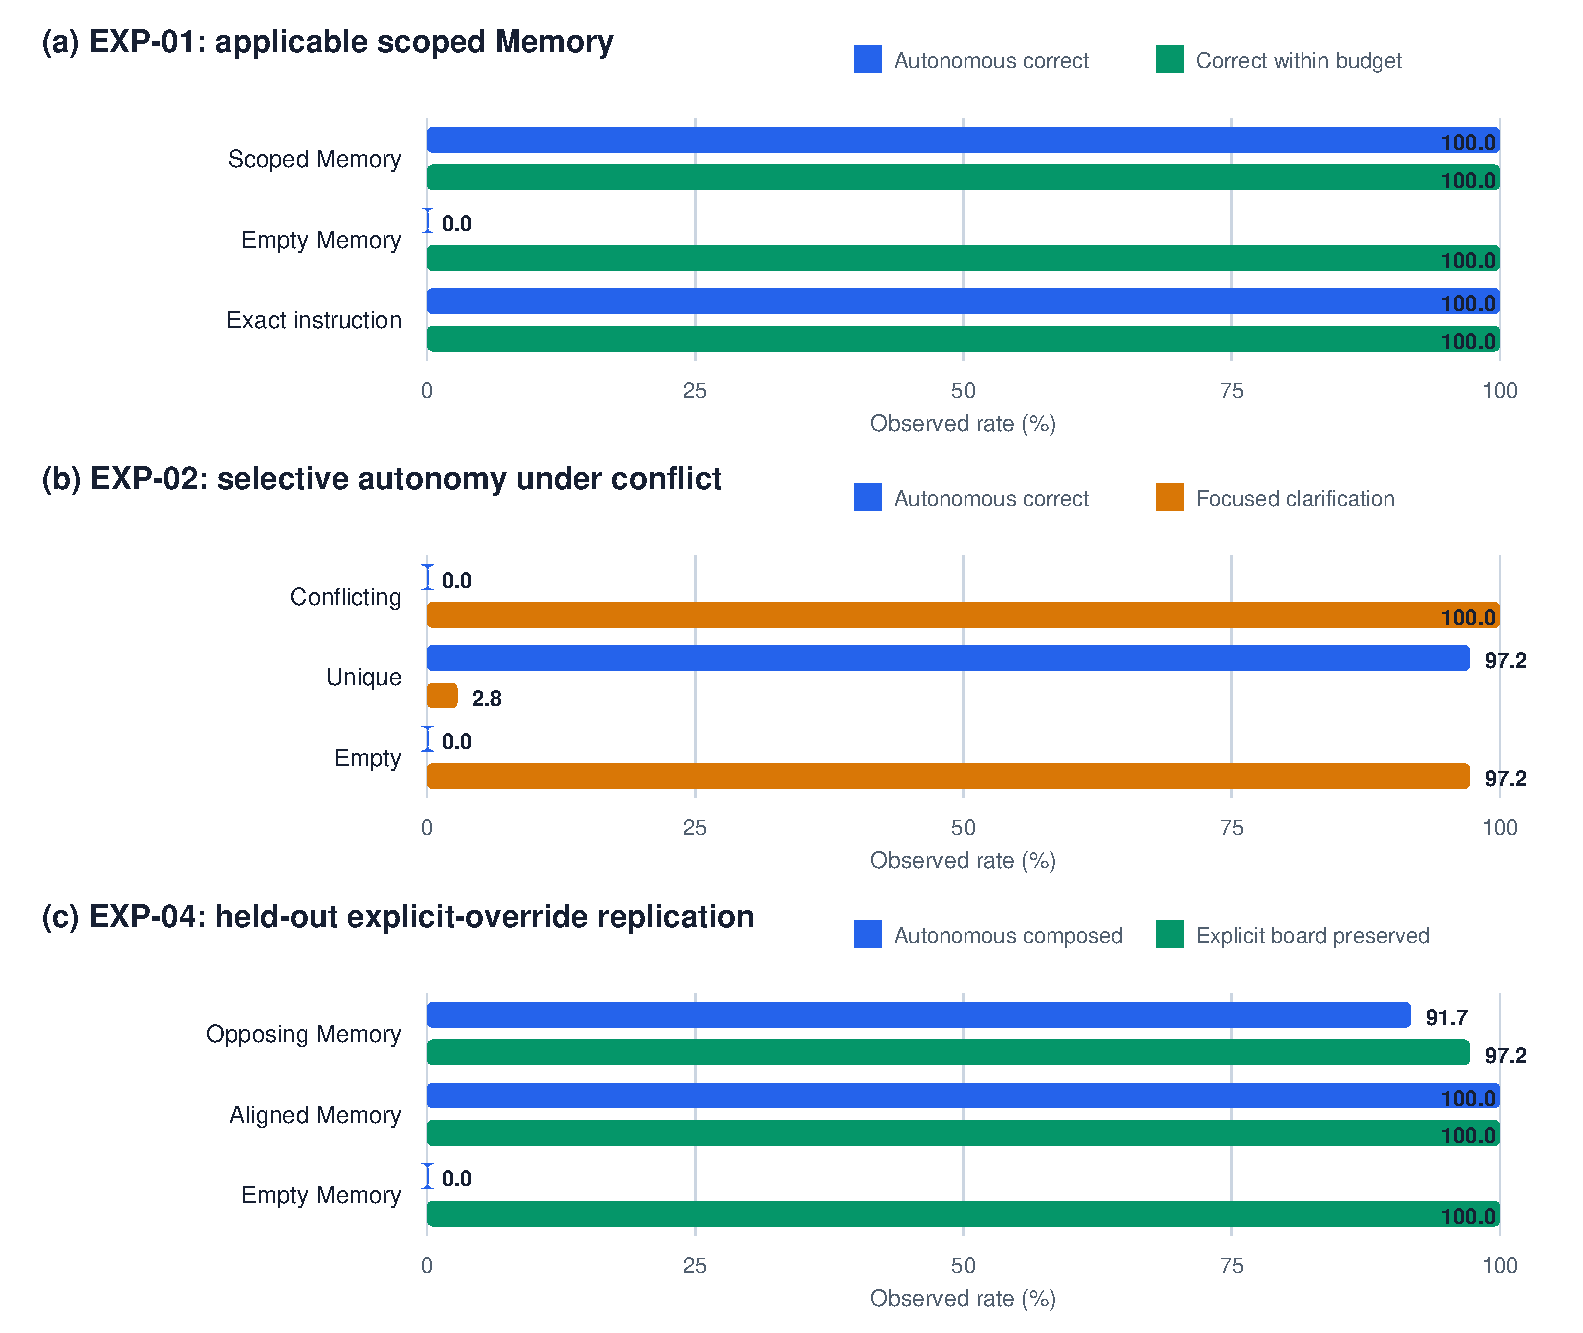
\includegraphics[width=\textwidth]{figures/evaluation-intent-results.pdf}
    \caption{Focused intent-resolution outcomes. Panel (a) distinguishes
    autonomy from attainable correctness; panel (b) shows selective autonomy
    under unique rather than conflicting evidence; panel (c) shows held-out
    explicit-current preservation.}
    \label{fig:app-intent-results}
\end{figure}

\subsection{Longitudinal Preference Lifecycle}

{\small
\renewcommand{\arraystretch}{1.12}
\begin{longtable}{@{}P{4.35cm}P{2.9cm}P{7.4cm}@{}}
    \caption{EXP-05 lifecycle outcomes across eight independent stores.}
    \label{tab:app-memory-lifecycle} \\
    \toprule
    \textbf{Operation} & \textbf{Direct outcome} & \textbf{Interpretation} \\
    \midrule
    \endfirsthead
    \caption[]{EXP-05 lifecycle outcomes (continued).} \\
    \toprule
    \textbf{Operation} & \textbf{Direct outcome} & \textbf{Interpretation} \\
    \midrule
    \endhead
    \bottomrule
    \endlastfoot
    Create initial preference & 8/8 & Initial authorised persistence succeeded. \\
    Immediate direct recall & 8/8 & Clean short-term retrieval ceiling. \\
    Initial HRI use & 8/8 & Retrieved value formed the correct no-motion goal. \\
    User isolation & 7/8 & One lifecycle crossed the registered ownership boundary. \\
    Task isolation and abstention & 7/8 each & Related task records were not
    perfectly isolated. \\
    Explicit update and ID preservation & 7/8 each & One update failed to retain
    the intended identity. \\
    Updated-value direct recall & 7/8 & Stored update was usually immediately
    retrievable. \\
    Updated HRI use & 5/8 & Correct retrieval did not always yield correct
    downstream staging. \\
    Delayed direct recall & 2/8 & Focal identity was often lost after related
    mutations. \\
    Delayed HRI use & 3/8 & One HRI goal was correct without the registered
    surviving-focal-record predicate. \\
    Revocation verified & 8/8 & The selected secondary record was absent after
    revocation, although only 2/8 revocation operations matched the intended
    focal lifecycle route. \\
    Final direct recall & 2/8 & Robust long-term preference preservation is not
    supported. \\
    Store consistency & 240/240 interactions & Serialization remained valid
    even when semantic identity was wrong. \\
\end{longtable}
}

\begin{figure}[H]
    \centering
    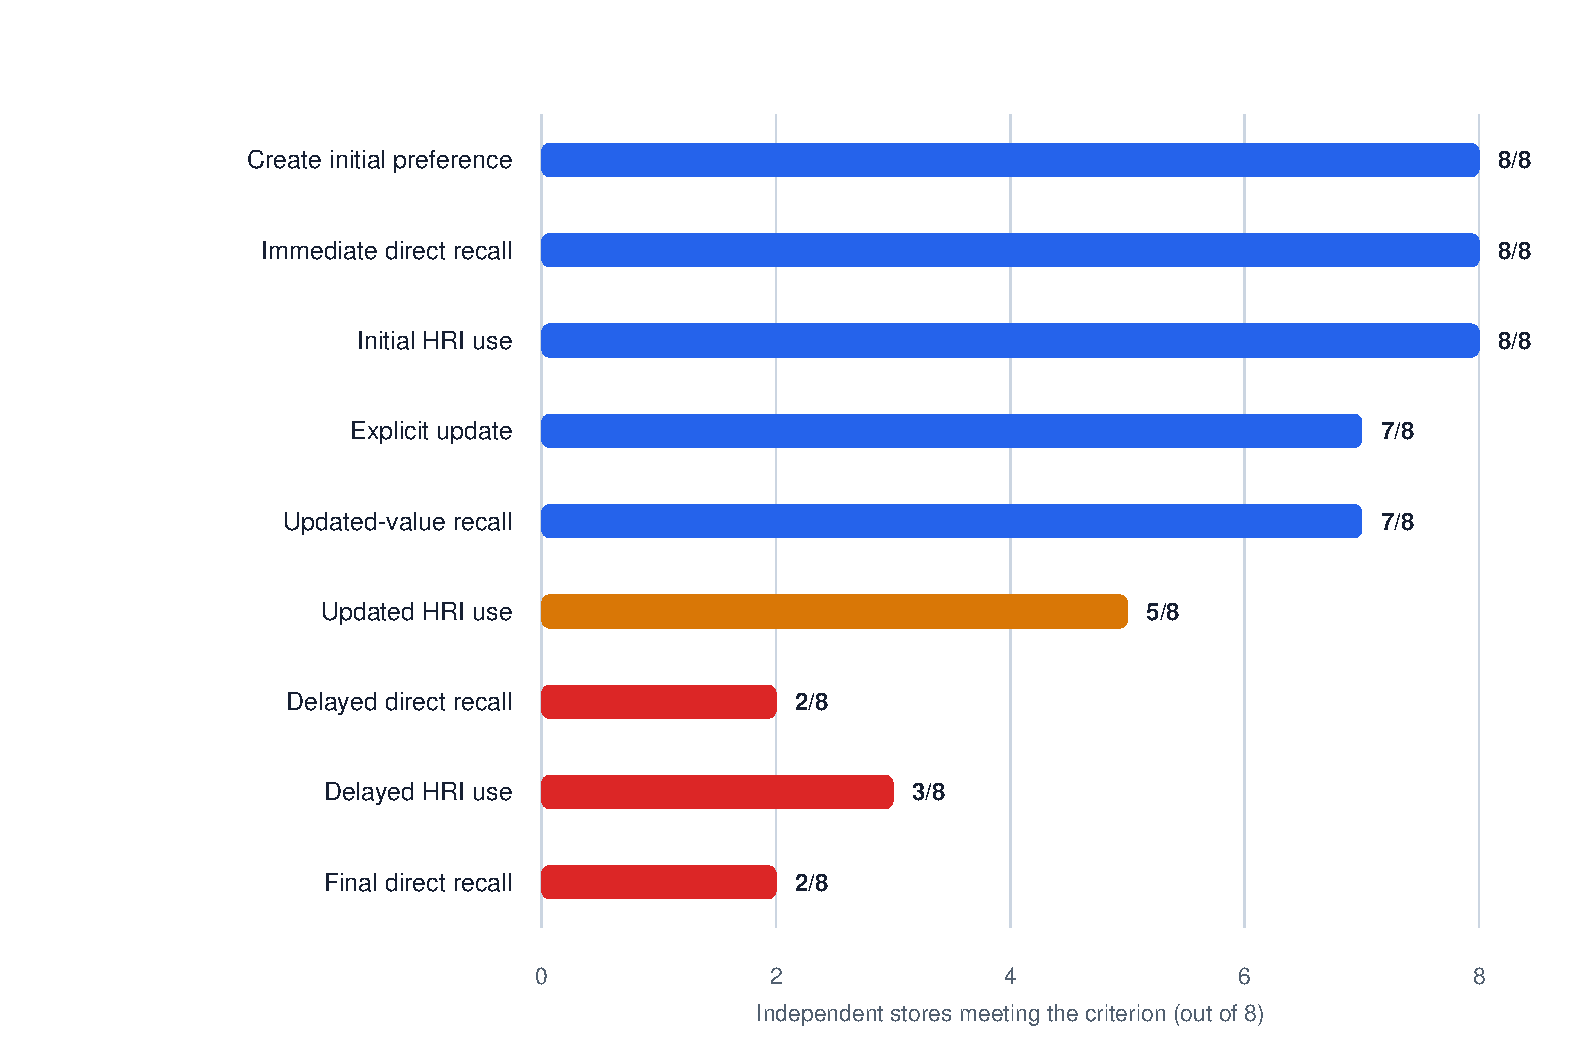
\includegraphics[width=\textwidth]{figures/evaluation-memory-lifecycle.pdf}
    \caption{EXP-05 lifecycle trajectory. Immediate creation and use were
    reliable, while delayed focal-record recall deteriorated after semantically
    related mutation pressure.}
    \label{fig:app-memory-lifecycle}
\end{figure}

\subsection{Monitor and Validator Ablations}

{\footnotesize
\renewcommand{\arraystretch}{1.1}
\begin{longtable}{@{}P{1.10cm}P{3.90cm}P{2.25cm}P{2.40cm}P{4.55cm}@{}}
    \caption{EXP-06 and EXP-07 paired ablation outcomes.}
    \label{tab:app-feedback-results} \\
    \toprule
    \textbf{Study} & \textbf{Outcome} & \textbf{Production} &
    \textbf{Control} & \textbf{Paired effect or interpretation} \\
    \midrule
    \endfirsthead
    \caption[]{Feedback-gate ablations (continued).} \\
    \toprule
    \textbf{Study} & \textbf{Outcome} & \textbf{Production} &
    \textbf{Control} & \textbf{Paired effect or interpretation} \\
    \midrule
    \endhead
    \bottomrule
    \endlastfoot
    EXP-06 & Expected host route & 22/36 & 12/36 & $+27.8$ pp; cluster 95\%
    interval $+8.3$ to $+50.0$ pp \\
    & Visual discrepancy recovery & 3/15 & 0/15 & $+20.0$ pp; weak absolute
    recovery \\
    & Stable endpoint transition & 7/9 & 0/9 & Clear visual endpoint contribution \\
    & Visible progress registered & 3/3 & 0/3 & Descriptive one-cluster effect \\
    & Safe hold / timeout & 6/6 and 3/3 & 6/6 and 3/3 & Deterministic host
    contribution, not learned Monitor gain \\
    & Schema-invalid attempts & 7/78 & 0 model calls & Retained as production
    capability observations \\
    EXP-07 & Expected final route & 35/36 & 15/36 & $+55.6$ pp; cluster 95\%
    interval $+25.0$ to $+83.3$ pp \\
    & False completion, incomplete & 0/21 & 21/21 & $-100$ pp \\
    & Correction requested, incomplete & 21/21 & 0/21 & $+100$ pp \\
    & Complete state finalised & 14/15 & 15/15 & $-6.7$ pp; one false
    rejection \\
    & Exact criterion vector & 34/36 & 15/36 & Descriptive localisation of
    visual disagreements \\
\end{longtable}
}

\begin{figure}[H]
    \centering
    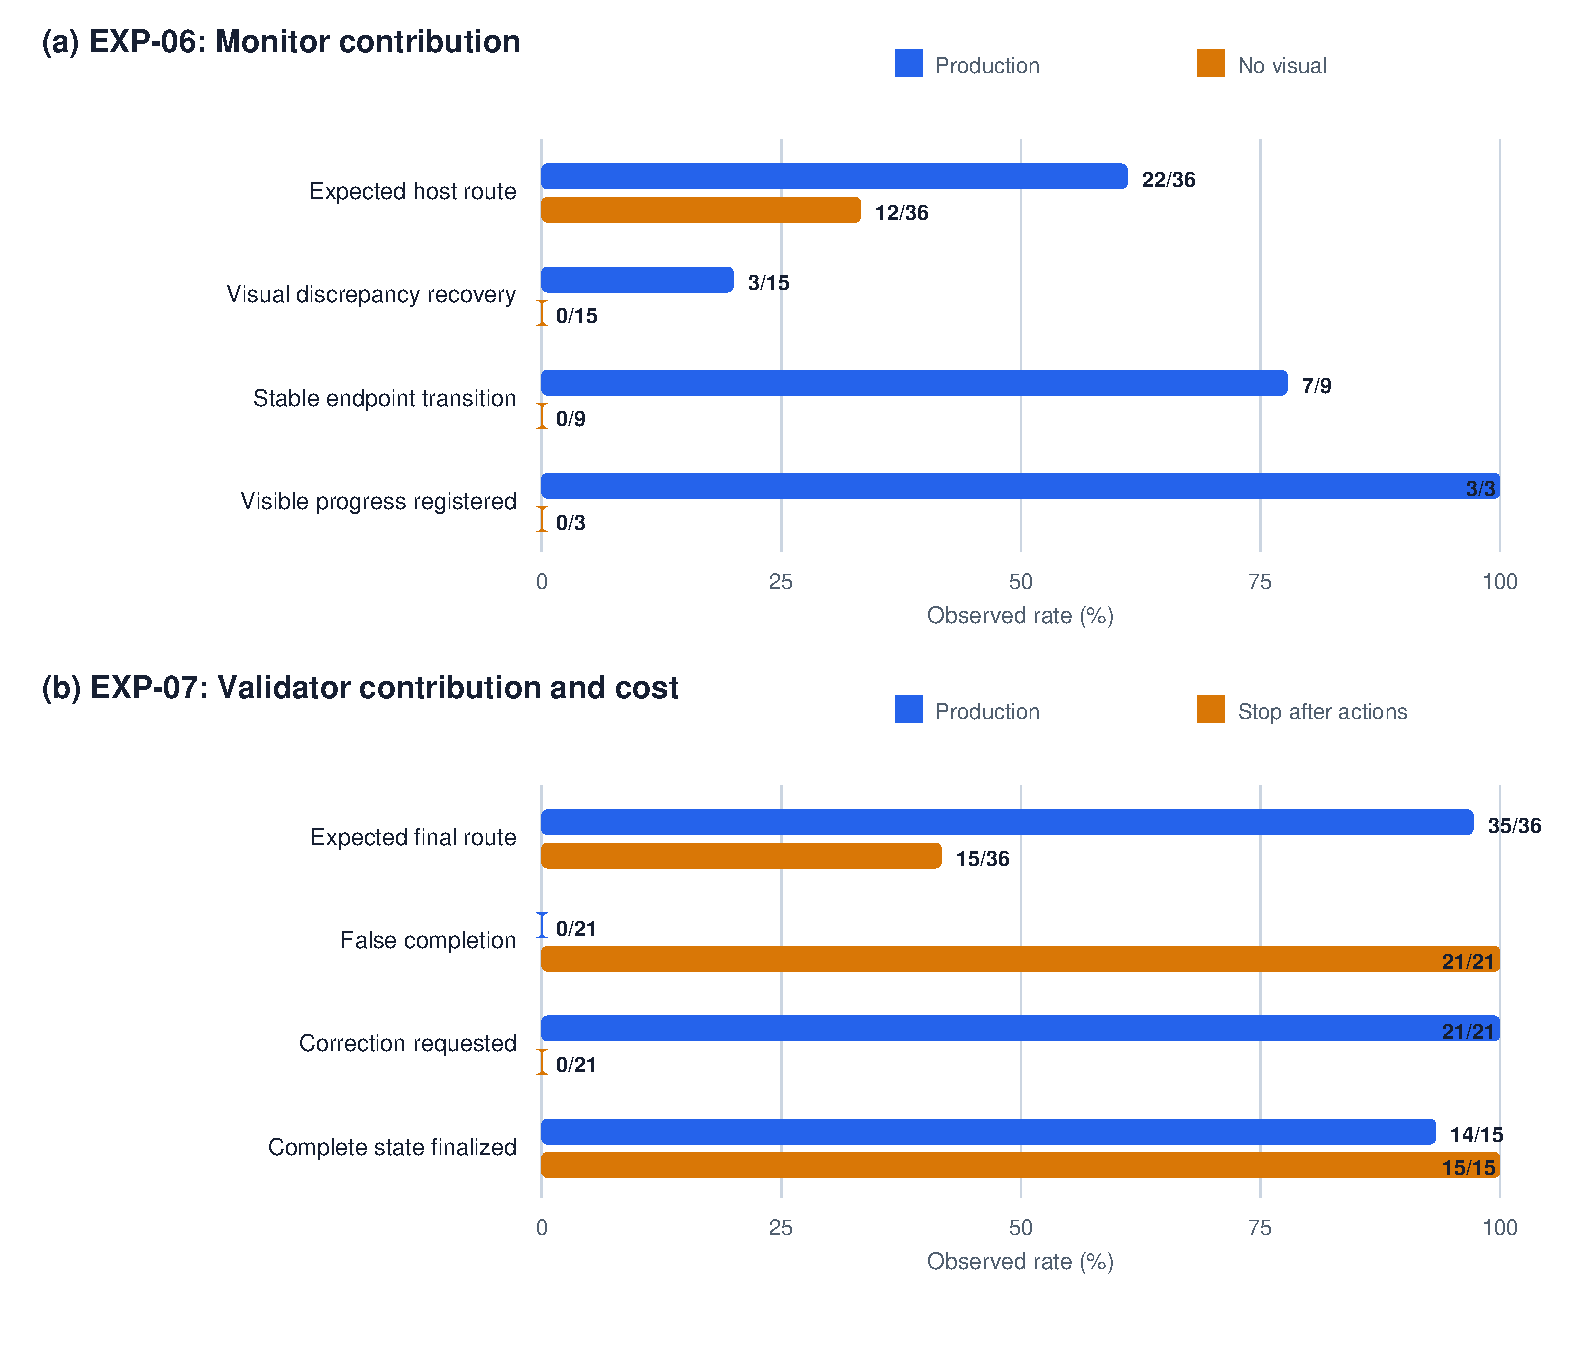
\includegraphics[width=\textwidth]{figures/evaluation-monitor-validator.pdf}
    \caption{Boundary-specific feedback effects. Monitor improved endpoints and
    progress more than discrepancy recovery; Validator prevented false
    completion at the cost of one controlled false rejection.}
    \label{fig:app-feedback-results}
\end{figure}

\subsection{Focused Six-Family Competency Envelope}

{\small
\renewcommand{\arraystretch}{1.12}
\begin{longtable}{@{}P{2.50cm}P{2.10cm}P{2.10cm}P{2.10cm}P{2.20cm}P{2.80cm}@{}}
    \caption{EXP-08 family-level outcomes.}
    \label{tab:app-competency-envelope} \\
    \toprule
    \textbf{Family} & \textbf{Registered event} & \textbf{Final outcome} &
    \textbf{Safety} & \textbf{Strict grounding} & \textbf{Oracle continuation} \\
    \midrule
    \endfirsthead
    \caption[]{EXP-08 family outcomes (continued).} \\
    \toprule
    \textbf{Family} & \textbf{Registered event} & \textbf{Final outcome} &
    \textbf{Safety} & \textbf{Strict grounding} & \textbf{Oracle continuation} \\
    \midrule
    \endhead
    \bottomrule
    \endlastfoot
    Slip & 2/3 & 2/3 & 3/3 & 2/2 attempted & 0/3 \\
    Timeout & 2/3 & 2/3 & 3/3 & 1/1 attempted & 1/3 \\
    Occlusion & 3/3 & 3/3 & 3/3 & 3/3 & 0/3 \\
    Planned outage & 3/3 & 3/3 & 3/3 & 3/3 & 0/3 \\
    Scoped preference & 3/3 & 3/3 & 3/3 & 3/3 & 0/3 \\
    Explicit override & 2/3 & 3/3 & 3/3 & 2/2 attempted & 1/3 \\
    \textbf{Overall} & \textbf{15/18} & \textbf{15/18} & \textbf{18/18} &
    \textbf{14 strict completions} & \textbf{2/18} \\
\end{longtable}
}

\subsection{Focused Simulated End to End}

{\footnotesize
\renewcommand{\arraystretch}{1.1}
\begin{longtable}{@{}P{2.60cm}P{3.40cm}P{3.10cm}P{1.80cm}P{2.80cm}@{}}
    \caption{EXP-09 contract-type outcomes. Every type obtained 3/3 expected
    Memory records, goal contracts, confirmations, correct first actions,
    physical goals, and safety.}
    \label{tab:app-end-to-end} \\
    \toprule
    \textbf{Contract type} & \textbf{Grounding / action count} &
    \textbf{Physical / Validator} & \textbf{Strict chain} &
    \textbf{Terminal states} \\
    \midrule
    \endfirsthead
    \caption[]{EXP-09 contract-type outcomes (continued).} \\
    \toprule
    \textbf{Contract type} & \textbf{Grounding / action count} &
    \textbf{Physical / Validator} & \textbf{Strict chain} &
    \textbf{Terminal states} \\
    \midrule
    \endhead
    \bottomrule
    \endlastfoot
    Omitted board & Strict 3/3; expected count 3/3 & Physical 3/3; Validator 3/3
    & 3/3 & COMPLETE: 3 \\
    Omitted cube & Strict 3/3; expected count 0/3 & Physical 3/3; Validator 0/3
    & 0/3 & NEEDS ATTENTION: 2; EXECUTING: 1 \\
    Explicit override & Strict 2/3; one assisted; expected count 2/3 & Physical
    3/3; Validator 3/3 & 2/3 & COMPLETE: 3 \\
    User scoped & Strict 3/3; expected count 3/3 & Physical 3/3; Validator 3/3
    & 3/3 & COMPLETE: 3 \\
    \textbf{Overall} & \textbf{Strict 11/12; expected count 8/12} &
    \textbf{Physical 12/12; Validator 9/12} & \textbf{8/12} & COMPLETE: 9;
    NEEDS ATTENTION: 2; EXECUTING: 1 \\
\end{longtable}
}

\begin{figure}[H]
    \centering
    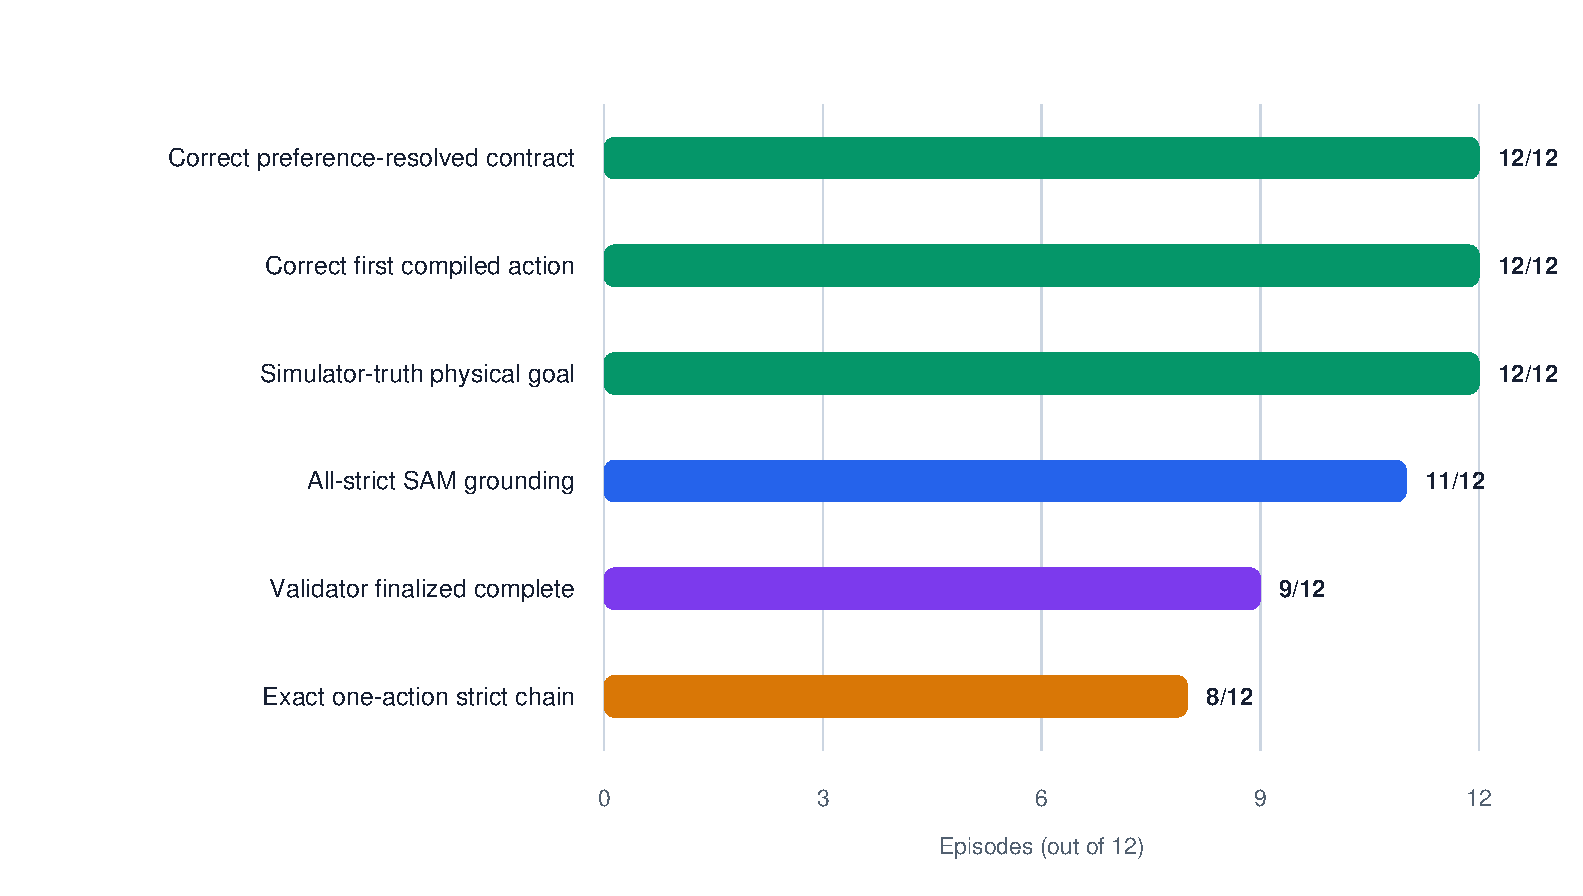
\includegraphics[width=\textwidth]{figures/evaluation-exp09-funnel.pdf}
    \caption{EXP-09 stage funnel. Contract and physical-state success remain
    distinct from all-strict grounding, Validator finalisation, and the exact
    one-action strict conjunction.}
    \label{fig:app-end-to-end-funnel}
\end{figure}


\clearpage
\section{Representative Structured Outputs and Failure Traces}
\label{app:representative-outputs}

Appendix Tables~\ref{tab:app-output-traces}
and~\ref{tab:app-output-authority} reproduce two retained EXP-09 observation
paths. They are examples, not additional trials. The first shows a complete
omitted-board chain. The second shows a physically correct omitted-cube
placement that did not receive visual finalisation and therefore repeated the
action before entering attention.

{\small
\renewcommand{\arraystretch}{1.12}
\begin{longtable}{@{}P{3.05cm}P{5.75cm}P{5.75cm}@{}}
    \caption{Representative successful and false-negative EXP-09 outputs.}
    \label{tab:app-output-traces} \\
    \toprule
    \textbf{Recorded field} & \textbf{Successful omitted-board episode} &
    \textbf{Physically correct omitted-cube episode} \\
    \midrule
    \endfirsthead
    \caption[]{Representative EXP-09 outputs (continued).} \\
    \toprule
    \textbf{Recorded field} & \textbf{Successful omitted-board episode} &
    \textbf{Physically correct omitted-cube episode} \\
    \midrule
    \endhead
    \bottomrule
    \endlastfoot
    Episode & \texttt{E2E-A-01, ctx-A01, var-09} &
    \texttt{E2E-A-02, ctx-A02, var-09} \\
    User utterance & ``Move red to whichever board my saved setting chooses.'' &
    ``Place the cube I routinely select in the middle of the cyan board.'' \\
    Expected Memory record & \texttt{A01-memory-01} & \texttt{A02-memory-01} \\
    Frozen actionable goal & Move the red cube to the cyan board; preserve all
    other cubes. & Place the blue cube at the centre of the cyan board. \\
    First compiler source/target & \texttt{red cube} / \texttt{cyan board} &
    \texttt{blue cube} / \texttt{cyan board} \\
    Memory, goal, and confirmation & All observed & All observed \\
    Strict grounding & True & True \\
    Physical actions & 1 & 3 \\
    Simulator-truth physical goal & True & True \\
    Validator complete & True & False \\
    Terminal state & \texttt{COMPLETE} & \texttt{NEEDS\_ATTENTION} \\
    Model calls / latency & 33 / 64.16 s & 98 / 138.79 s \\
    Scientific interpretation & Complete preference-to-physical-state and
    evidence chain. & Intent and motion were correct, but a low-contrast
    blue-on-cyan visual false negative caused repetition and bounded attention. \\
\end{longtable}
}

\begingroup
\footnotesize
\begin{verbatim}
Successful structured output (abridged)
  memory_lookup_observed: true
  expected_memory_records_observed: true
  goal_contract_correct: true
  confirmation_observed: true
  first_source_query: red cube
  first_target_query: cyan board
  physical_action_count: 1
  strict_grounding_completed: true
  physical_goal_satisfied: true
  validator_finalized_complete: true
  terminal_runtime_state: COMPLETE

False-negative structured output (abridged)
  memory_lookup_observed: true
  expected_memory_records_observed: true
  goal_contract_correct: true
  confirmation_observed: true
  first_source_query: blue cube
  first_target_query: cyan board
  physical_action_count: 3
  strict_grounding_completed: true
  physical_goal_satisfied: true
  validator_finalized_complete: false
  terminal_runtime_state: NEEDS_ATTENTION
\end{verbatim}
\endgroup

{\small
\renewcommand{\arraystretch}{1.12}
\begin{longtable}{@{}P{3.0cm}P{5.7cm}P{5.9cm}@{}}
    \caption{Authority used to score the representative output fields.}
    \label{tab:app-output-authority} \\
    \toprule
    \textbf{Stage} & \textbf{Recorded evidence} & \textbf{Scoring authority} \\
    \midrule
    \endfirsthead
    \caption[]{Representative-output scoring authority (continued).} \\
    \toprule
    \textbf{Stage} & \textbf{Recorded evidence} & \textbf{Scoring authority} \\
    \midrule
    \endhead
    \bottomrule
    \endlastfoot
    Preference & Lookup trace and exact returned record IDs & Frozen expected
    record list; no simulator state \\
    Contract & Goal proposal, ID/revision, confirmation event & Registered
    semantic contract and host confirmation record \\
    First action & Compiler source and target queries & Registered expected
    pick/place program \\
    Grounding & Strict SAM/RGB-D attempt and optional assisted lineage & Strict
    call record; assistance never repairs the strict flag \\
    Physical state & Settled object pose and distractor state & Hidden MuJoCo
    state used only after execution for scoring \\
    Monitoring and validation & Publication-bound assessments and final report &
    Ordinary third-person frames plus typed host aggregation \\
    Terminal status & Controller state, guards, and immutable history &
    Deterministic host state machine \\
\end{longtable}
}


\clearpage
\section{Supplementary Main-Body Tables}
\label{app:main-body-tables}

\subsection{Related-System Positioning}

{\small
\renewcommand{\arraystretch}{1.14}
\begin{longtable}{@{}P{2.35cm}P{4.00cm}P{3.75cm}P{4.35cm}@{}}
    \caption{Comparison of related personalised and agentic robot systems.
    ``Adaptation'' refers to changes beyond the immediate inference context.}
    \label{tab:related-system-comparison} \\
    \toprule
    \textbf{System} &
    \textbf{Preference or interaction evidence} &
    \textbf{Execution feedback} &
    \textbf{Principal distinction from PrefMem} \\
    \midrule
    \endfirsthead
    \caption[]{Comparison of related personalised and agentic robot systems
    (continued).} \\
    \toprule
    \textbf{System} &
    \textbf{Preference or interaction evidence} &
    \textbf{Execution feedback} &
    \textbf{Principal distinction from PrefMem} \\
    \midrule
    \endhead
    \midrule
    \multicolumn{4}{r@{}}{\small Continued on next page} \\
    \endfoot
    \bottomrule
    \endlastfoot

    TidyBot \parencite{wu2023tidybot} &
    Examples summarised into personalised placement and primitive rules. &
    Repeated perception and execution during cleanup. &
    Focuses on preference generalisation rather than consented record
    lifecycle, exact confirmation, or independent final validation. \\

    LLM-Personalize \parencite{han2024llmpersonalize} &
    Demonstrations and preference-labelled self-training data. &
    Iterative planning from a scene graph. &
    Personalises the planner through optimisation rather than an explicit
    persistent record store. \\

    APRICOT \parencite{wang2024apricot} &
    Visual demonstrations and active preference queries. &
    World-model feedback and constraint-aware plan refinement. &
    Learns among candidate preferences; PrefMem governs explicit persistent
    records, conflicts, overrides, and consent. \\

    KnowNo \parencite{ren2023knowno} &
    Ambiguity represented as a calibrated action prediction set. &
    Human help is requested when the set is not a singleton. &
    Provides conformal calibration; PrefMem instead separates semantic,
    historical, and execution attention states. \\

    Hi Robot \parencite{shi2025hirobot} &
    Current prompts, observations, and mid-task user feedback. &
    High-level VLM repeatedly instructs a low-level VLA. &
    Does not centre persistent preference provenance or exact goal-contract
    confirmation. \\

    Agentic Robot \parencite{yang2025agenticrobot} &
    High-level task instruction and visual observations. &
    Temporal verification, retry, and recovery for planned subgoals. &
    PrefMem adds consented preference memory, horizon-one fresh replanning,
    and a separate whole-goal Validator. \\

    MEM \parencite{torne2026mem} &
    Within-episode video history and semantic event summaries. &
    Memory conditions high- and low-level VLA policies. &
    Addresses embodied task memory rather than cross-interaction user
    preference authority. \\

    RoboClaw \parencite{li2026roboclaw} &
    Structured task and working memory. &
    Tool-based skill monitoring, retry, recovery, and human escalation. &
    Unifies execution with data and policy refinement; PrefMem keeps model
    weights fixed and separates execution history from user preference memory. \\

    PrefMem &
    Explicitly mutable, scoped preference records plus current user input. &
    One published task, temporally fenced Monitor evidence, fresh replanning,
    and independent final validation. &
    Studies preference provenance, exact goal authorisation, deterministic
    state ownership, and evidence-gated terminal decisions as one inspectable
    orchestration boundary. \\
\end{longtable}
}

\subsection{Architectural Alternatives}

\begin{table}[H]
    \centering
    \small
    \caption{Architectural trade-off between a monolithic tool-using agent and
    PrefMem's role-specialised graph.}
    \label{tab:architecture-alternatives}
    \begin{tabular}{@{}P{3.1cm}P{5.5cm}P{5.5cm}@{}}
        \toprule
        \textbf{Criterion} & \textbf{Monolithic agent} &
        \textbf{Role-specialised PrefMem} \\
        \midrule
        Model residency & One loaded model & One shared loaded model; logical
        roles do not duplicate weights \\
        Prompt and tools & Union of all histories, instructions, schemas, and
        tools & Role-specific context and least-authority tool surfaces \\
        State ownership & Primarily model/conversation mediated & Deterministic
        runtime and controller own authoritative state \\
        Temporal behaviour & One loop multiplexes dialogue, observation, and
        control & Separate user-turn, planning, monitoring, validation, and
        execution loops \\
        Verification & Planner can influence or certify its own result &
        Separate Monitor and Validator evidence routes; host derives completion \\
        Testability & End-to-end behaviour is simpler but failures are opaque &
        Components, interfaces, and host policies can be tested separately \\
        Cost & Fewer calls and lower orchestration overhead & More calls,
        schemas, latency, and integration complexity \\
        \bottomrule
    \end{tabular}
\end{table}

\subsection{Interaction Contracts}

\begin{table}[H]
    \centering
    \small
    \caption{Principal interaction contracts and authority boundaries.}
    \label{tab:interaction-contracts}
    \begin{tabular}{@{}P{2.5cm}P{2.7cm}P{4.4cm}P{4.4cm}@{}}
        \toprule
        \textbf{Source} & \textbf{Destination} & \textbf{Artifact} &
        \textbf{Authority rule} \\
        \midrule
        User & HRI & Request, clarification, confirmation, guidance & User
        authorises ambiguous semantics and persistence \\
        HRI & Memory & Labelled retrieve or mutate request & Memory can return
        or change only request-valid records \\
        HRI & Runtime & Preview, confirm, resume, or replan tool call & Runtime
        validates state and exact identifiers \\
        Runtime & Planner & Preview payload or \texttt{PlannerCycleRequest} &
        Planner proposes; host assigns IDs and selects task one \\
        Runtime & Monitor & \texttt{STEP} \texttt{PublishedTask} & Monitor
        observes only the current step \\
        Runtime & Validator & Goal for compilation or final publication &
        Validator cannot rewrite goal or host-derived status \\
        Runtime & Executor & \texttt{STEP} \texttt{PublishedTask} & Executor
        changes the scene but cannot establish completion \\
        Monitor / Validator & Runtime / Controller & Typed assessment or error &
        Identity, time, phase, and criteria must match \\
        Controller & Planner & Immutable \texttt{ExecutionRecord} on next cycle
        & Only host code appends trusted history \\
        Runtime & HRI & State summary, attention cause, validation report & HRI
        reports but cannot fabricate recovery authority \\
        \bottomrule
    \end{tabular}
\end{table}

\subsection{Requirement-to-Evidence Traceability}

{\small
\renewcommand{\arraystretch}{1.12}
\begin{longtable}{@{}P{1.35cm}P{4.25cm}P{4.20cm}P{4.15cm}@{}}
    \caption{Requirement-to-mechanism and evidence traceability.}
    \label{tab:requirement-traceability} \\
    \toprule
    \textbf{Req.} & \textbf{Primary mechanism} &
    \textbf{Principal evidence} & \textbf{Important boundary} \\
    \midrule
    \endfirsthead
    \caption[]{Requirement-to-mechanism and evidence traceability
    (continued).} \\
    \toprule
    \textbf{Req.} & \textbf{Primary mechanism} &
    \textbf{Principal evidence} & \textbf{Important boundary} \\
    \midrule
    \endhead
    \midrule
    \multicolumn{4}{r@{}}{\small Continued on next page} \\
    \endfoot
    \bottomrule
    \endlastfoot

    R1 & HRI ambiguity policy, scoped Memory use, focused clarification &
    \texttt{C-HRI-AMB}, interfaces, EXP-01 and EXP-02 & Selected tabletop
    field resolution, not open-world intent understanding \\
    R2 & Retrieval provenance, request-scoped mutation guards, explicit-current
    priority & \texttt{C-MEM}, EXP-02 through EXP-05 & Free-text identity and
    scope remain longitudinal limitations \\
    R3 & Host goal ID/revision and exact confirmation tool & HRI tool and state
    tests, EXP-01--04 and EXP-09 & Confirmation is per run and is not memory
    consent \\
    R4 & Stateless Planner, fresh frames, candidate-one selection, terminal
    history & \texttt{C-PLN}, workflow ladder, \texttt{AB-RPL-F/T} & Host
    ablations do not establish learned Planner quality \\
    R5 & Publication IDs, generations, phase and frame-sequence checks &
    \texttt{C-MON-ERR}, \texttt{C-VAL-RESET}, interaction tests & Fencing does
    not correct a semantically wrong but schema-valid assessment \\
    R6 & Repeated success/failure evidence and stability duration &
    \texttt{C-MON-STABLE}, EXP-06 & Visual label quality limits what host
    aggregation can stabilise \\
    R7 & Frozen ValidationContract and host-derived broad status &
    \texttt{C-VAL}, EXP-07 and EXP-09 & Prevents false completion but may cause
    false rejection \\
    R8 & Attention state, timeout records, repetition and cycle guards &
    \texttt{PF-REPLAN/SAFETY}, \texttt{AB-RPL-T}, EXP-08 & Software recovery
    policy, not hardware safety certification \\
    R9 & Narrow PublishedTask boundary and human/MuJoCo adapters &
    \texttt{C-EXE}, calibration, EXP-08 and EXP-09 & Current adapter is not a
    learned VLA \\
    R10 & Typed contracts, immutable attempts, traces, manifests, direct staged
    metrics & All suite layers and focused reports & Original suite remains
    development/non-confirmatory evidence \\
\end{longtable}
}

Generative AI was used to correct writing, improve phrasing, fix bugs, and draw the diagrams.
\printbibliography

\end{document}
